% !TeX spellcheck = hu_HU
% !TeX encoding = UTF-8
% !TeX program = xelatex
\documentclass[11pt,a4paper,oneside]{report}             % Single-side
%\documentclass[11pt,a4paper,twoside,openright]{report}  % Duplex

% thanks to http://tex.stackexchange.com/a/47579/71109
\usepackage{ifxetex}
\usepackage{ifluatex}
\newif\ifxetexorluatex % a new conditional starts as false
\ifnum 0\ifxetex 1\fi\ifluatex 1\fi>0
   \xetexorluatextrue
\fi

\ifxetexorluatex
  \usepackage{fontspec}
\else
  \usepackage[T1]{fontenc}
  \usepackage[utf8]{inputenc}
  \usepackage[lighttt]{lmodern}
\fi

\usepackage[english,magyar]{babel} % Alapértelmezés szerint utoljára definiált nyelv lesz aktív, de később külön beállítjuk az aktív nyelvet.

%\usepackage{cmap}
\usepackage{amsfonts,amsmath,amssymb} % Mathematical symbols.
%\usepackage[ruled,boxed,resetcount,linesnumbered]{algorithm2e} % For pseudocodes. % beware: this is not compatible with LuaLaTeX, see http://tex.stackexchange.com/questions/34814/lualatex-and-algorithm2e
\usepackage{booktabs} % For publication quality tables for LaTeX
\usepackage{graphicx}

%\usepackage{fancyhdr}
%\usepackage{lastpage}

\usepackage{anysize}
%\usepackage{sectsty}
\usepackage{setspace} % For setting line spacing

\usepackage[unicode]{hyperref} % For hyperlinks in the generated document.
\usepackage{xcolor}
\usepackage{listings} % For source code snippets.

\usepackage[amsmath,thmmarks]{ntheorem} % Theorem-like environments.

\usepackage[hang]{caption}

\singlespacing

\newcommand{\selecthungarian}{
	\selectlanguage{magyar}
	\setlength{\parindent}{2em}
	\setlength{\parskip}{0em}
	\frenchspacing
}

\newcommand{\selectenglish}{
	\selectlanguage{english}
	\setlength{\parindent}{0em}
	\setlength{\parskip}{0.5em}
	\nonfrenchspacing
	\renewcommand{\figureautorefname}{Figure}
	\renewcommand{\tableautorefname}{Table}
	\renewcommand{\partautorefname}{Part}
	\renewcommand{\chapterautorefname}{Chapter}
	\renewcommand{\sectionautorefname}{Section}
	\renewcommand{\subsectionautorefname}{Section}
	\renewcommand{\subsubsectionautorefname}{Section}
}

\usepackage[numbers]{natbib}
\usepackage{xspace}
\usepackage{amssymb}% to access $\blacksquare$
\usepackage{multirow}


%TODO Set the main variables
\newcommand{\vikszerzoVezeteknev}{Jost}
\newcommand{\vikszerzoKeresztnev}{Márk Benedek}

\newcommand{\vikkonzulensAMegszolitas}{Dr.~}
\newcommand{\vikkonzulensAVezeteknev}{Szegletes}
\newcommand{\vikkonzulensAKeresztnev}{Luca}

\newcommand{\vikkonzulensBMegszolitas}{}
\newcommand{\vikkonzulensBVezeteknev}{}
\newcommand{\vikkonzulensBKeresztnev}{}

\newcommand{\vikkonzulensCMegszolitas}{}
\newcommand{\vikkonzulensCVezeteknev}{}
\newcommand{\vikkonzulensCKeresztnev}{}

\newcommand{\vikcim}{Útvonaltervezési algoritmusok optimalizálása GPU-n} % Cím
\newcommand{\viktanszek}{\bmeaut} % Tanszék
\newcommand{\vikdoktipus}{\bsc} % Dokumentum típusa (\bsc vagy \msc)
\newcommand{\vikmunkatipusat}{szakdolgozatot} % a "hallgató nyilatkozat" részhez: szakdolgozatot vagy diplomatervet

%%--------------------------------------------------------------------------------------
% TDK-specifikus változók
%--------------------------------------------------------------------------------------
\newcommand{\tdkszerzoB}{Második Szerző} % Második szerző neve; hagyd üresen, ha egyedül írtad a TDK-t.
\newcommand{\tdkev}{2014} % A dolgozat írásának éve (pl. "2014") (Ez OTDK-nál eltérhet az aktuális évtől.)

% További adatok az OTDK címlaphoz (BME-s TDK-hoz nem kell kitölteni)
\newcommand{\tdkevfolyamA}{IV} % Első szerző évfolyama, római számmal (pl. IV).
\newcommand{\tdkevfolyamB}{III} % Második szerző évfolyama, római számmal (pl. III).
\newcommand{\tdkkonzulensbeosztasA}{egyetemi tanár} % Első konzulens beosztása (pl. egyetemi docens)
\newcommand{\tdkkonzulensbeosztasB}{doktorandusz} % Második konzulens beosztása (pl. egyetemi docens)
 % Csak ha tdk készül
\newcommand{\szerzoMeta}{\vikszerzoVezeteknev{} \vikszerzoKeresztnev} % egy szerző esetén
%\newcommand{\szerzoMeta}{\vikszerzoVezeteknev{} \vikszerzoKeresztnev, \tdkszerzoB} % két szerző esetén

% Beállítások magyar nyelvű dolgozathoz
%--------------------------------------------------------------------------------------
% Elnevezések
%--------------------------------------------------------------------------------------
\newcommand{\bme}{Budapesti Műszaki és Gazdaságtudományi Egyetem}
\newcommand{\vik}{Villamosmérnöki és Informatikai Kar}

\newcommand{\bmeaut}{Automatizálási és Alkalmazott Informatikai Tanszék}

\newcommand{\keszitette}{Készítette}
\newcommand{\konzulens}{Konzulens}

\newcommand{\bsc}{Szakdolgozat}
\newcommand{\msc}{Diplomaterv}
\newcommand{\tdk}{TDK dolgozat}
\newcommand{\bsconlab}{BSc Önálló laboratórium}
\newcommand{\msconlabi}{MSc Önálló laboratórium 1.}
\newcommand{\msconlabii}{MSc Önálló laboratórium 2.}

\newcommand{\pelda}{Példa}
\newcommand{\definicio}{Definíció}
\newcommand{\tetel}{Tétel}

\newcommand{\bevezetes}{Bevezetés}
\newcommand{\koszonetnyilvanitas}{Köszönetnyilvánítás}
\newcommand{\fuggelek}{Függelék}

% Opcionálisan átnevezhető címek
%\addto\captionsmagyar{%
%\renewcommand{\listfigurename}{Saját ábrajegyzék cím}
%\renewcommand{\listtablename}{Saját táblázatjegyzék cím}
%\renewcommand{\bibname}{Saját irodalomjegyzék név}
%}

\newcommand{\szerzo}{\vikszerzoVezeteknev{} \vikszerzoKeresztnev}
\newcommand{\vikkonzulensA}{\vikkonzulensAMegszolitas\vikkonzulensAVezeteknev{} \vikkonzulensAKeresztnev}
\newcommand{\vikkonzulensB}{\vikkonzulensBMegszolitas\vikkonzulensBVezeteknev{} \vikkonzulensBKeresztnev}
\newcommand{\vikkonzulensC}{\vikkonzulensCMegszolitas\vikkonzulensCVezeteknev{} \vikkonzulensCKeresztnev}

\newcommand{\selectthesislanguage}{\selecthungarian}

\bibliographystyle{huplain}

\def\lstlistingname{lista}

\newcommand{\appendixnumber}{6}  % a fofejezet-szamlalo az angol ABC 6. betuje (F) lesz

% Settings for English documents
%%--------------------------------------------------------------------------------------
% Elnevezések
%--------------------------------------------------------------------------------------
\newcommand{\bme}{Budapesti Műszaki és Gazdaságtudományi Egyetem}
\newcommand{\vik}{Faculty of Electrical Engineering and Informatics}

\newcommand{\bmemit}{Department of Measurement and Information Systems}

\newcommand{\keszitette}{Author}
\newcommand{\konzulens}{Advisor}

\newcommand{\bsc}{Bachelor's Thesis}
\newcommand{\msc}{Master's Thesis}
\newcommand{\tdk}{Scientific Students' Association Report}
\newcommand{\bsconlab}{BSc Project Laboratory}
\newcommand{\msconlabi}{MSc Project Laboratory 1}
\newcommand{\msconlabii}{MSc Project Laboratory 2}

\newcommand{\pelda}{Example}
\newcommand{\definicio}{Definition}
\newcommand{\tetel}{Theorem}

\newcommand{\bevezetes}{Introduction}
\newcommand{\koszonetnyilvanitas}{Acknowledgements}
\newcommand{\fuggelek}{Appendix}

% Optional custom titles
%\addto\captionsenglish{%
%\renewcommand*{\listfigurename}{Your list of figures title}
%\renewcommand*{\listtablename}{Your list of tables title}
%\renewcommand*{\bibname}{Your bibliography title}
%}

\newcommand{\szerzo}{\vikszerzoKeresztnev{} \vikszerzoVezeteknev}
\newcommand{\vikkonzulensA}{\vikkonzulensAMegszolitas\vikkonzulensAKeresztnev{} \vikkonzulensAVezeteknev}
\newcommand{\vikkonzulensB}{\vikkonzulensBMegszolitas\vikkonzulensBKeresztnev{} \vikkonzulensBVezeteknev}
\newcommand{\vikkonzulensC}{\vikkonzulensCMegszolitas\vikkonzulensCKeresztnev{} \vikkonzulensCVezeteknev}

\newcommand{\selectthesislanguage}{\selectenglish}

\bibliographystyle{plainnat}

\newcommand{\ie}{i.e.\@\xspace}
\newcommand{\Ie}{I.e.\@\xspace}
\newcommand{\eg}{e.g.\@\xspace}
\newcommand{\Eg}{E.g.\@\xspace}
\newcommand{\etal}{et al.\@\xspace}
\newcommand{\etc}{etc.\@\xspace}
\newcommand{\vs}{vs.\@\xspace}
\newcommand{\viz}{viz.\@\xspace} % videlicet
\newcommand{\cf}{cf.\@\xspace} % confer
\newcommand{\Cf}{Cf.\@\xspace}
\newcommand{\wrt}{w.r.t.\@\xspace} % with respect to
\newcommand{\approximately}{approx.\@\xspace}

\newcommand{\appendixnumber}{1}  % a fofejezet-szamlalo az angol ABC 1. betuje (A) lesz


%--------------------------------------------------------------------------------------
% Page layout setup
%--------------------------------------------------------------------------------------
% we need to redefine the pagestyle plain
% another possibility is to use the body of this command without \fancypagestyle
% and use \pagestyle{fancy} but in that case the special pages
% (like the ToC, the References, and the Chapter pages)remain in plane style

\pagestyle{plain}
\marginsize{35mm}{25mm}{15mm}{15mm}

\setcounter{tocdepth}{3}
%\sectionfont{\large\upshape\bfseries}
\setcounter{secnumdepth}{3}

\sloppy % Margón túllógó sorok tiltása.
\widowpenalty=10000 \clubpenalty=10000 %A fattyú- és árvasorok elkerülése
\def\hyph{-\penalty0\hskip0pt\relax} % Kötőjeles szavak elválasztásának engedélyezése


%--------------------------------------------------------------------------------------
% Setup hyperref package
%--------------------------------------------------------------------------------------
\hypersetup{
    % bookmarks=true,            % show bookmarks bar?
    unicode=true,              % non-Latin characters in Acrobat's bookmarks
    pdftitle={\vikcim},        % title
    pdfauthor={\szerzoMeta},    % author
    pdfsubject={\vikdoktipus}, % subject of the document
    pdfcreator={\szerzoMeta},   % creator of the document
    pdfproducer={},    % producer of the document
    pdfkeywords={},    % list of keywords (separate then by comma)
    pdfnewwindow=true,         % links in new window
    colorlinks=true,           % false: boxed links; true: colored links
    linkcolor=black,           % color of internal links
    citecolor=black,           % color of links to bibliography
    filecolor=black,           % color of file links
    urlcolor=black             % color of external links
}


%--------------------------------------------------------------------------------------
% Set up listings
%--------------------------------------------------------------------------------------
\definecolor{lightgray}{rgb}{0.95,0.95,0.95}
\lstset{
	basicstyle=\scriptsize\ttfamily, % print whole listing small
	keywordstyle=\color{black}\bfseries, % bold black keywords
	identifierstyle=, % nothing happens
	% default behavior: comments in italic, to change use
	% commentstyle=\color{green}, % for e.g. green comments
	stringstyle=\scriptsize,
	showstringspaces=false, % no special string spaces
	aboveskip=3pt,
	belowskip=3pt,
	backgroundcolor=\color{lightgray},
	columns=flexible,
	keepspaces=true,
	escapeinside={(*@}{@*)},
	captionpos=b,
	breaklines=true,
	frame=single,
	float=!ht,
	tabsize=2,
	literate=*
		{á}{{\'a}}1	{é}{{\'e}}1	{í}{{\'i}}1	{ó}{{\'o}}1	{ö}{{\"o}}1	{ő}{{\H{o}}}1	{ú}{{\'u}}1	{ü}{{\"u}}1	{ű}{{\H{u}}}1
		{Á}{{\'A}}1	{É}{{\'E}}1	{Í}{{\'I}}1	{Ó}{{\'O}}1	{Ö}{{\"O}}1	{Ő}{{\H{O}}}1	{Ú}{{\'U}}1	{Ü}{{\"U}}1	{Ű}{{\H{U}}}1
}

%--------------------------------------------------------------------------------------
% Source code listings
%--------------------------------------------------------------------------------------
\definecolor{mGreen}{rgb}{0,0.6,0}
\definecolor{mGray}{rgb}{0.5,0.5,0.5}
\definecolor{mPurple}{rgb}{0.58,0,0.82}
\definecolor{backgroundColour}{rgb}{0.95,0.95,0.92}

\lstdefinestyle{CStyle}{
	backgroundcolor=\color{backgroundColour},   
	commentstyle=\color{mGreen},
	keywordstyle=\color{magenta},
	numberstyle=\tiny\color{mGray},
	stringstyle=\color{mPurple},
	basicstyle=\footnotesize,
	breakatwhitespace=false,         
	breaklines=true,                 
	captionpos=b,                    
	keepspaces=true,                 
	numbers=none,                    
	numbersep=5pt,                  
	showspaces=false,                
	showstringspaces=true,
	extendedchars=true,
	literate      =        % Support additional characters
	{á}{{\'a}}1  {é}{{\'e}}1  {í}{{\'i}}1 {ó}{{\'o}}1 {ő}{{\csname u8:\detokenize{ő}\endcsname}}1 {ú}{{\'u}}1  {ű}{{\csname u8:\detokenize{ű}\endcsname}}1
	{Á}{{\'A}}1  {É}{{\'E}}1  {Í}{{\'I}}1 {Ó}{{\'O}}1  {Ő}{{\csname u8:\detokenize{Ő}\endcsname}}1 {Ú}{{\'U}}1 {Ű}{{\csname u8:\detokenize{Ű}\endcsname}}1
	{ä}{{\"a}}1  {ë}{{\"e}}1  {ï}{{\"i}}1 {ö}{{\"o}}1  {ü}{{\"u}}1
	{Ä}{{\"A}}1  {Ë}{{\"E}}1  {Ï}{{\"I}}1 {Ö}{{\"O}}1  {Ü}{{\"U}}1
	{ê}{{\^e}}1,
	inputencoding=utf8,
	showtabs=false,                  
	tabsize=2,
	language=C++
}

%--------------------------------------------------------------------------------------
% Set up theorem-like environments
%--------------------------------------------------------------------------------------
% Using ntheorem package -- see http://www.math.washington.edu/tex-archive/macros/latex/contrib/ntheorem/ntheorem.pdf

\theoremstyle{plain}
\theoremseparator{.}
\newtheorem{example}{\pelda}

\theoremseparator{.}
%\theoremprework{\bigskip\hrule\medskip}
%\theorempostwork{\hrule\bigskip}
\theorembodyfont{\upshape}
\theoremsymbol{{\large \ensuremath{\centerdot}}}
\newtheorem{definition}{\definicio}

\theoremseparator{.}
%\theoremprework{\bigskip\hrule\medskip}
%\theorempostwork{\hrule\bigskip}
\newtheorem{theorem}{\tetel}


%--------------------------------------------------------------------------------------
% Some new commands and declarations
%--------------------------------------------------------------------------------------
\newcommand{\code}[1]{{\upshape\ttfamily\scriptsize\indent #1}}
\newcommand{\doi}[1]{DOI: \href{http://dx.doi.org/\detokenize{#1}}{\raggedright{\texttt{\detokenize{#1}}}}} % A hivatkozások közt így könnyebb DOI-t megadni.

\DeclareMathOperator*{\argmax}{arg\,max}
%\DeclareMathOperator*[1]{\floor}{arg\,max}
\DeclareMathOperator{\sign}{sgn}
\DeclareMathOperator{\rot}{rot}


%--------------------------------------------------------------------------------------
% Setup captions
%--------------------------------------------------------------------------------------
\captionsetup[figure]{
	width=.75\textwidth,
	aboveskip=10pt}

\renewcommand{\captionlabelfont}{\bf}
%\renewcommand{\captionfont}{\footnotesize\it}

%--------------------------------------------------------------------------------------
% Hyphenation exceptions
%--------------------------------------------------------------------------------------
\hyphenation{Shakes-peare Mar-seilles ár-víz-tű-rő tü-kör-fú-ró-gép}


\author{\vikszerzo}
\title{\viktitle}

%--------------------------------------------------------------------------------------
% Table of contents and the main text
%--------------------------------------------------------------------------------------
\begin{document}

\pagenumbering{gobble}

%TODO These includes define guidelines -- remove these
%~~~~~~~~~~~~~~~~~~~~~~~~~~~~~~~~~~~~~~~~~~~~~~~~~~~~~~~~~~~~~~~~~~~~~~~~~~~~~~~~~~~~~~
%\selecthungarian
%--------------------------------------------------------------------------------------
% Rovid formai es tartalmi tajekoztato
%--------------------------------------------------------------------------------------

\footnotesize
\begin{center}
\large
\textbf{\Large Általános információk, a diplomaterv szerkezete}\\
\end{center}

A diplomaterv szerkezete a BME Villamosmérnöki és Informatikai Karán:
\begin{enumerate}
\item	Diplomaterv feladatkiírás
\item	Címoldal
\item	Tartalomjegyzék
\item	A diplomatervező nyilatkozata az önálló munkáról és az elektronikus adatok kezeléséről
\item	Tartalmi összefoglaló magyarul és angolul
\item	Bevezetés: a feladat értelmezése, a tervezés célja, a feladat indokoltsága, a diplomaterv felépítésének rövid összefoglalása
\item	A feladatkiírás pontosítása és részletes elemzése
\item	Előzmények (irodalomkutatás, hasonló alkotások), az ezekből levonható következtetések
\item	A tervezés részletes leírása, a döntési lehetőségek értékelése és a választott megoldások indoklása
\item	A megtervezett műszaki alkotás értékelése, kritikai elemzése, továbbfejlesztési lehetőségek
\item	Esetleges köszönetnyilvánítások
\item	Részletes és pontos irodalomjegyzék
\item	Függelék(ek)
\end{enumerate}

Felhasználható a következő oldaltól kezdődő \LaTeX diplomatervsablon dokumentum tartalma. 

A diplomaterv szabványos méretű A4-es lapokra kerüljön. Az oldalak tükörmargóval készüljenek (mindenhol 2,5~cm, baloldalon 1~cm-es kötéssel). Az alapértelmezett betűkészlet a 12 pontos Times New Roman, másfeles sorközzel, de ettől kismértékben el lehet térni, ill. más betűtípus használata is megengedett.

Minden oldalon -- az első négy szerkezeti elem kivételével -- szerepelnie kell az oldalszámnak.

A fejezeteket decimális beosztással kell ellátni. Az ábrákat a megfelelő helyre be kell illeszteni, fejezetenként decimális számmal és kifejező címmel kell ellátni. A fejezeteket decimális aláosztással számozzuk, maximálisan 3 aláosztás mélységben (pl. 2.3.4.1.). Az ábrákat, táblázatokat és képleteket célszerű fejezetenként külön számozni (pl. 2.4. ábra, 4.2. táblázat vagy képletnél (3.2)). A fejezetcímeket igazítsuk balra, a normál szövegnél viszont használjunk sorkiegyenlítést. Az ábrákat, táblázatokat és a hozzájuk tartozó címet igazítsuk középre. A cím a jelölt rész alatt helyezkedjen el.

A képeket lehetőleg rajzoló programmal készítsék el, az egyenleteket egyenlet-szerkesztő segítségével írják le (A \LaTeX~ehhez kézenfekvő megoldásokat nyújt).

Az irodalomjegyzék szövegközi hivatkozása történhet sorszámozva (ez a preferált megoldás) vagy a Harvard-rendszerben (a szerző és az évszám megadásával). A teljes lista névsor szerinti sorrendben a szöveg végén szerepeljen (sorszámozott irodalmi hivatkozások esetén hivatkozási sorrendben). A szakirodalmi források címeit azonban mindig az eredeti nyelven kell megadni, esetleg zárójelben a fordítással. A listában szereplő valamennyi publikációra hivatkozni kell a szövegben (a \LaTeX-sablon a Bib\TeX~segítségével mindezt automatikusan kezeli). Minden publikáció a szerzők után a következő adatok szerepelnek: folyóirat cikkeknél a pontos cím, a folyóirat címe, évfolyam, szám, oldalszám tól-ig. A folyóiratok címét csak akkor rövidítsük, ha azok nagyon közismertek vagy nagyon hosszúak. Internetes hivatkozások megadásakor fontos, hogy az elérési út előtt megadjuk az oldal tulajdonosát és tartalmát (mivel a link egy idő után akár elérhetetlenné is válhat), valamint az elérés időpontját.

\vspace{5mm}
Fontos:
\begin{itemize}
	\item A szakdolgozatkészítő / diplomatervező nyilatkozata (a jelen sablonban szereplő szövegtartalommal) kötelező előírás, Karunkon ennek hiányában a szakdolgozat/diplomaterv nem bírálható és nem védhető!
	\item Mind a dolgozat, mind a melléklet maximálisan 15~MB méretű lehet!
\end{itemize}

\vspace{5mm}
\begin{center}
Jó munkát, sikeres szakdolgozatkészítést, ill. diplomatervezést kívánunk!
\end{center}

\normalsize
\selectthesislanguage

%%--------------------------------------------------------------------------------------
% Feladatkiiras (a tanszeken atveheto, kinyomtatott valtozat)
%--------------------------------------------------------------------------------------
\clearpage
\begin{center}
\large
\textbf{FELADATKIÍRÁS}\\
\end{center}

A feladatkiírást a tanszéki adminisztrációban lehet átvenni, és a leadott munkába eredeti, tanszéki pecséttel ellátott és a tanszékvezető által aláírt lapot kell belefűzni (ezen oldal \emph{helyett}, ez az oldal csak útmutatás). Az elektronikusan feltöltött dolgozatban már nem kell beleszerkeszteni ezt a feladatkiírást.


\selectthesislanguage

%~~~~~~~~~~~~~~~~~~~~~~~~~~~~~~~~~~~~~~~~~~~~~~~~~~~~~~~~~~~~~~~~~~~~~~~~~~~~~~~~~~~~~~
\hypersetup{pageanchor=false}
%--------------------------------------------------------------------------------------
%	The title page
%--------------------------------------------------------------------------------------
\begin{titlepage}
\begin{center}

\includegraphics[width=60mm,keepaspectratio]{figures/bme_logo.pdf}\\
\vspace{0.3cm}
\textbf{\bme}\\
\textmd{\vik}\\
\textmd{\viktanszek}\\[5cm]

\vspace{0.4cm}
{\huge \bfseries \vikcim}\\[0.8cm]
\vspace{0.5cm}
\textsc{\Large \vikdoktipus}\\[4cm]

{
	\renewcommand{\arraystretch}{0.85}
	\begin{tabular}{cc}
	 \makebox[7cm]{\emph{\keszitette}} & \makebox[7cm]{\emph{\konzulens}} \\ \noalign{\smallskip}
	 \makebox[7cm]{\szerzo} & \makebox[7cm]{\vikkonzulensA} \\
	  & \makebox[7cm]{\vikkonzulensB} \\
	  & \makebox[7cm]{\vikkonzulensC} \\
	\end{tabular}
}

\vfill
{\large \today}
\end{center}
\end{titlepage}
\hypersetup{pageanchor=false}

		   % Szakdolgozat/Diplomaterv címlap
%%% TDK címlap
\begin{titlepage}
  \begin{center}  
  
\includegraphics[width=7cm]{./figures/bme_logo.pdf}
  \vspace{0.3cm}
  
  \bme \\
  \vik \\
  \viktanszek \\
  \vspace{5cm}
  
  \huge {\vikcim}
  \vspace{1.5cm}
  
  \large {\textbf{\tdk}}
  \vfill
    
  {\Large 
  	\keszitette: \\ \vspace{0.3cm}
  	\szerzo \\
	\tdkszerzoB \\
  	\vspace{1.5cm}
  	\konzulens: \\ \vspace{0.3cm}
  	\vikkonzulensA \\
  	\vikkonzulensB \\
  }
  
  \vspace{2cm}
  \large {\tdkev}
 \end{center}
\end{titlepage}
%% Címlap vége
	% TDK címlap
%%% OTDK külső címlap
\begin{titlepage}
  	$\;$ 
	\vspace{5cm}
	
	\begin{center}
	\Huge
	\textbf{TDK-dolgozat}\let\thefootnote\relax\footnote{A dolgozat bemutatását a XXXXXXXXX  ``Lorem ipsum dolor sit amet'' című program támogatta.}
	\end{center}
	
	\vspace{13cm}
	
	\Large
	\hspace{8cm} \szerzo
	
	\hspace{8cm} \tdkszerzoB
	
	\hspace{8cm} \tdkev.
\end{titlepage}

\newpage
\thispagestyle{empty}


%% OTDK belső címlap
\begin{titlepage}
  \begin{center}  
  
\includegraphics[width=7cm]{./figures/bme_logo.pdf}
  \vspace{0.3cm}
  
  \bme \\
  \vik \\
  \viktanszek \\
  \vspace{3.5cm}
  
  \huge {\vikcim}
  \vspace{1.5cm}
  
  \large {\textbf{\vikdoktipus}}
  \vfill
    
  {\Large 
  	{\large \keszitette:} \\ \vspace{0.2cm}
  	\szerzo \\ \tdkevfolyamA. évfolyam \\
	\vspace{0.5cm}
	\tdkszerzoB \\ \tdkevfolyamB. évfolyam \\
  	\vspace{1.5cm}
  	{\large \konzulens:} \\ \vspace{0.2cm}
  	\vikkonzulensA,\\ \tdkkonzulensbeosztasA \\
  	\vspace{0.5cm}
  	\vikkonzulensB,\\ \tdkkonzulensbeosztasB \\
  }
  
  \vspace{2cm}
  \large {\tdkev.}
  
 \end{center}
\end{titlepage}   % OTDK címlap


% Table of Contents
%~~~~~~~~~~~~~~~~~~~~~~~~~~~~~~~~~~~~~~~~~~~~~~~~~~~~~~~~~~~~~~~~~~~~~~~~~~~~~~~~~~~~~~
\tableofcontents\vfill


% Declaration and Abstract
%~~~~~~~~~~~~~~~~~~~~~~~~~~~~~~~~~~~~~~~~~~~~~~~~~~~~~~~~~~~~~~~~~~~~~~~~~~~~~~~~~~~~~~
\selectlanguage{magyar}
\pagenumbering{gobble}
%--------------------------------------------------------------------------------------
% Nyilatkozat
%--------------------------------------------------------------------------------------
\begin{center}
\large
\textbf{HALLGATÓI NYILATKOZAT}\\
\end{center}

Alulírott \emph{\vikszerzoVezeteknev{} \vikszerzoKeresztnev}, szigorló hallgató kijelentem, hogy ezt a \vikmunkatipusat{} meg nem engedett segítség nélkül, saját magam készítettem, csak a megadott forrásokat (szakirodalom, eszközök stb.) használtam fel. Minden olyan részt, melyet szó szerint, vagy azonos értelemben, de átfogalmazva más forrásból átvettem, egyértelműen, a forrás megadásával megjelöltem.

Hozzájárulok, hogy a jelen munkám alapadatait (szerző(k), cím, angol és magyar nyelvű tartalmi kivonat, készítés éve, konzulens(ek) neve) a BME VIK nyilvánosan hozzáférhető elektronikus formában, a munka teljes szövegét pedig az egyetem belső hálózatán keresztül (vagy autentikált felhasználók számára) közzétegye. Kijelentem, hogy a benyújtott munka és annak elektronikus verziója megegyezik. Dékáni engedéllyel titkosított diplomatervek esetén a dolgozat szövege csak 3 év eltelte után válik hozzáférhetővé.

\begin{flushleft}
\vspace*{1cm}
Budapest, \today
\end{flushleft}

\begin{flushright}
 \vspace*{1cm}
 \makebox[7cm]{\rule{6cm}{.4pt}}\\
 \makebox[7cm]{\emph{\vikszerzoVezeteknev{} \vikszerzoKeresztnev}}\\
 \makebox[7cm]{hallgató}
\end{flushright}
\thispagestyle{empty}

\vfill
\clearpage
\thispagestyle{empty} % an empty page

\selectthesislanguage
 
\pagenumbering{roman}
\setcounter{page}{1}

\selecthungarian

%----------------------------------------------------------------------------
% Abstract in Hungarian
%----------------------------------------------------------------------------
\chapter*{Kivonat}\addcontentsline{toc}{chapter}{Kivonat}

Különböző hálózatok, legyen az egy szociális média felhasználói hálója, egy ország közúthálózata, de akár egy NYÁK-terven a különböző komponensek vezetékezése során alapvető problémák az úgynevezett útkeresési problémák (Vehicle Routing Problems - VRP). Ezek bizonyítottan NP-nehéz problémák, a megoldásuk egy költséges, ugyanakkor gyakran monoton tevékenység, hiszen sok pontsorozat hossza közül kell kiválasztani a legrövidebbet. Dolgozatom célja a Hangyakolónia Optimalizáció (Ant Colony Optimization - ACO) elvével egy heurisztikus, vagyis valószínűségi megoldás találása. Az ACO nagymértékben párhuzamosítható, melyet azzal tudtam kihasználni, hogy videokártyán összehangolt threadek ezreit voltam képes futtatni az NVIDIA CUDA keretrendszer segítségével. A készült kódot C/C++ nyelven valósítottam meg.

%TODO Abstractot megírni

\vfill
\selectenglish


%----------------------------------------------------------------------------
% Abstract in English
%----------------------------------------------------------------------------
\chapter*{Abstract}\addcontentsline{toc}{chapter}{Abstract}

This document is a \LaTeX-based skeleton for BSc/MSc~theses of students at the Electrical Engineering and Informatics Faculty, Budapest University of Technology and Economics. The usage of this skeleton is optional. It has been tested with the \emph{TeXLive} \TeX~implementation, and it requires the PDF-\LaTeX~compiler.


\vfill
\selectthesislanguage

\newcounter{romanPage}
\setcounter{romanPage}{\value{page}}
\stepcounter{romanPage}    


% The main part of the thesis
%~~~~~~~~~~~~~~~~~~~~~~~~~~~~~~~~~~~~~~~~~~~~~~~~~~~~~~~~~~~~~~~~~~~~~~~~~~~~~~~~~~~~~~
\pagenumbering{arabic}

%TODO import your own content
%TODO Ne legyen hivatkozás címben
%TODO törtek egységesen vagy , vagy .-tal jelölve
%TODO Táblázatok és leírások konzisztensek legyenek
%TODO Táblázatok leírása
%TODO Vízszintes vonalak a repek közé
%TODO NVIDIA trademark jelölés?
%%----------------------------------------------------------------------------
\chapter{\bevezetes}
%----------------------------------------------------------------------------

A bevezető tartalmazza a diplomaterv-kiírás elemzését, történelmi előzményeit, a feladat indokoltságát (a motiváció leírását), az eddigi megoldásokat, és ennek tükrében a hallgató megoldásának összefoglalását.

A bevezető szokás szerint a diplomaterv felépítésével záródik, azaz annak rövid leírásával, hogy melyik fejezet mivel foglalkozik.

%%----------------------------------------------------------------------------
\chapter{\LaTeX-eszközök}
\label{sec:LatexTools}
%----------------------------------------------------------------------------
\section{A szerkesztéshez használatos eszközök}
%----------------------------------------------------------------------------
Ez a sablon TeXstudio 2.8.8 szerkesztővel készült. A TeXstudio egy platformfüggetlen, Windows, Linux és Mac OS alatt is elérhető \LaTeX-szerkesztőprogram számtalan hasznos szolgáltatással (\refstruc{fig:TeXstudio}). A szoftver ingyenesen letölthető\footnote{A TeXstudio hivatalos oldala: \url{http://texstudio.sourceforge.net/}}.

\begin{figure}[!ht]
\centering
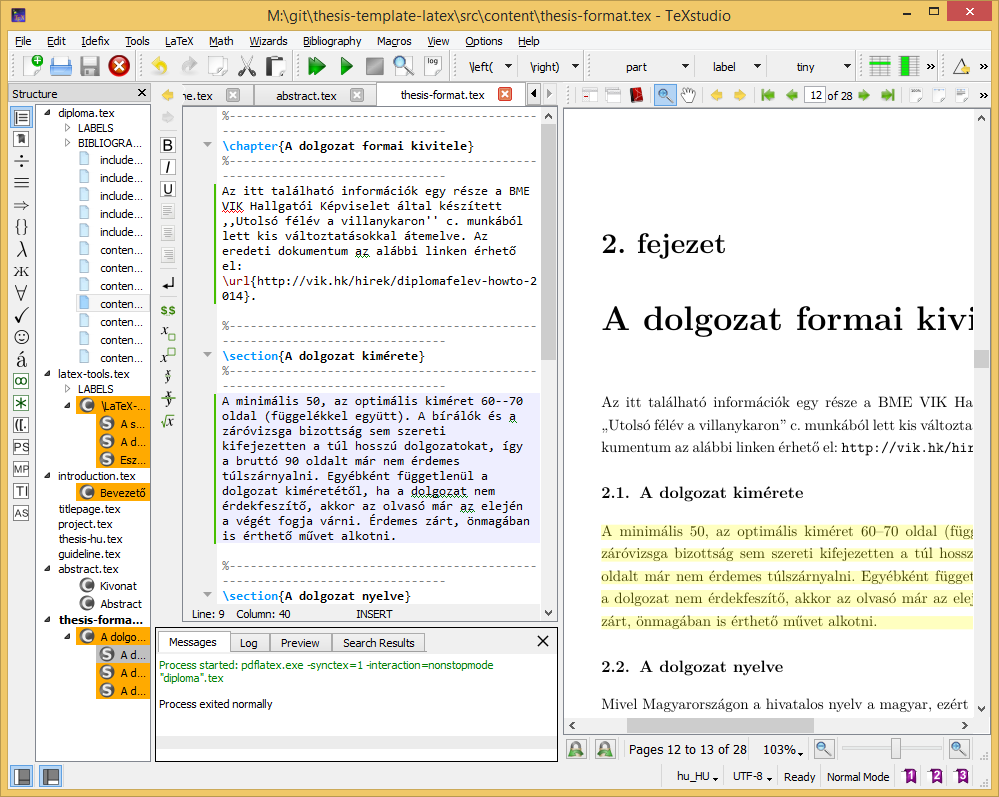
\includegraphics[width=150mm, keepaspectratio]{figures/TeXstudio.png}
\caption{A TeXstudio \LaTeX-szerkesztő.}
\label{fig:TeXstudio}
\end{figure}

A TeXstudio telepítése után érdemes még letölteni a magyar nyelvű helyesírásellenőrző-szótárakat hozzá. A TeXstudio az OpenOffice-hoz használatos formátumot tudja kezelni. A TeXstudio beállításainál a \verb+General+ fülön a \verb+Dictionaries+ résznél tudjuk megadni, hogy melyik szótárat használja.

Egy másik használható Windows alapú szerkesztőprogram a LEd\footnote{A LEd hivatalos oldala: \url{http://www.latexeditor.org/}} (LaTeX Editor), a TeXstudio azonban stabilabb, gyorsabb, és jobban használható.

%----------------------------------------------------------------------------
\section{A dokumentum lefordítása Windows alatt}
%----------------------------------------------------------------------------
A TeXstudio és a LEd kizárólag szerkesztőprogram (bár az utóbbiban DVI-nézegető is van), így a dokumentum fordításához szükséges eszközöket nem tartalmazza. Windows alatt alapvetően két lehetőség közül érdemes választani: MiKTeX (\url{http://miktex.org/}) és TeX Live (\url{http://www.tug.org/texlive/}) programcsomag. Az utóbbi működik Mac OS X, GNU/Linux alatt és Unix-származékokon is. A MiKTeX egy alapcsomag telepítése után mindig letölti a használt funkciókhoz szükséges, de lokálisan hiányzó \TeX-csomagokat, míg a TeX Live DVD ISO verzóban férhető hozzá. Ez a dokumentum TeX Live 2008 programcsomag segítségével fordult, amelynek DVD ISO verziója a megadott oldalról letölthető. A sablon lefordításához a disztribúcióban szereplő \verb+magyar.ldf+ fájlt a \verb+http://www.math.bme.hu/latex/+ változatra kell cserélni, vagy az utóbbi változatot be kell másolni a projekt-könyvtárba (ahogy ezt meg is tettük a sablonban) különben anomáliák tapasztalhatók a dokumentumban (pl. az ábra- és táblázat-aláírások formátuma nem a beállított lesz, vagy bizonyos oldalakon megjelenik alapértelmezésben egy fejléc). A TeX Live 2008-at még nem kell külön telepíteni a gépre, elegendő DVD-ről (vagy az ISO fájlból közvetlenül, pl. DaemonTools-szal) használni.

Ha a MiKTeX csomagot használjuk, akkor parancssorból a következő módon tudjuk újrafordítani a teljes dokumentumot:

\begin{lstlisting}[language=bash,frame=single,float=!ht]
$ texify -p thesis.tex
\end{lstlisting}

A \verb+texify+ parancs a MiKTex programcsomag \verb+miktex/bin+ alkönyvtárában található. A parancs gondoskodik arról, hogy a szükséges lépéseket (fordítás, hivatkozások generálása stb.) a megfelelő sorrendben elvégezze. A \verb+-p+ kapcsoló hatására PDF-et generál. A fordítást és az ideiglenes fájlok törlését elvégezhetjük a sablonhoz mellékelt \verb+manual_build.bat+ szkript segítségével is.

A \TeX-eszközöket tartalmazó programcsomag binárisainak elérési útját gyakran be kell állítani a szerkesztőprogramban, például TeXstudio esetén legegyszerűbben az \verb+Options / Configure TeXstudio... / Commands+ menüponttal előhívott dialógusablakban tehetjük ezt meg.

A PDF-\LaTeX~használata esetén a generált dokumentum közvetlenül PDF-formátumban áll rendelkezésre. Amennyiben a PDF-fájl egy PDF-nézőben (pl. Adobe Acrobat Reader vagy Foxit PDF Reader) meg van nyitva, akkor a fájlleírót a PDF-néző program tipikusan lefoglalja. Ilyen esetben a dokumentum újrafordítása hibaüzenettel kilép. Ha bezárjuk és újra megnyitjuk a PDF dokumentumot, akkor pedig a PDF-nézők többsége az első oldalon nyitja meg a dokumentumot, nem a legutóbb olvasott oldalon. Ezzel szemben például az egyszerű és ingyenes \textcolor{blue}{Sumatra PDF} nevű program képes arra, hogy a megnyitott dokumentum megváltozását detektálja, és frissítse a nézetet az aktuális oldal megtartásával.

%----------------------------------------------------------------------------
\section{Eszközök Linuxhoz}
%----------------------------------------------------------------------------
Linux operációs rendszer alatt is rengeteg szerkesztőprogram van, pl. a KDE alapú Kile jól használható. Ez ingyenesen letölthető, vagy éppenséggel az adott Linux-disztribúció eleve tartalmazza, ahogyan a dokumentum fordításához szükséges csomagokat is. Az Ubuntu Linux disztribúciók alatt például legtöbbször a \verb+texlive-*+ csomagok telepítésével használhatók a \LaTeX-eszközök. A jelen sablon fordításához szükséges csomagok (kb. 0,5 GB) az alábbi paranccsal telepíthetők:

\begin{lstlisting}[language=bash,morekeywords={sudo,apt\-get},alsoletter={-},breaklines=true]
$ sudo apt-get install texlive-latex-extra texlive-fonts-extra texlive-fonts-recommended texlive-xetex texlive-science
\end{lstlisting}

Amennyiben egy újabb csomag hozzáadása után hiányzó fájlra utaló hibát kapunk a fordítótól, telepítenünk kell az azt tartalmazó TeX Live csomagot. Ha pl. a \verb+bibentry+ csomagot szeretnénk használni, futtassuk az alábbi parancsot:

\begin{lstlisting}[language=bash,morekeywords={apt\-cache},alsoletter={-},breaklines=true]
$ apt-cache search bibentry
texlive-luatex - TeX Live: LuaTeX packages
\end{lstlisting}

Majd telepítsük fel a megfelelő TeX Live csomagot, jelen esetben a `texlive-lualatex`-et. (Egy LaTeX csomag több TeX Live csomagban is szerepelhet.)

Ha gyakran szerkesztünk más \LaTeX dokumentumokat is, kényelmes és biztos megoldás a teljes TeX Live disztribúció telepítése, ez azonban kb. 4 GB helyet igényel.

\begin{lstlisting}[language=bash,morekeywords={sudo,apt\-get},alsoletter={-},breaklines=true]
sudo apt-get install texlive-full
\end{lstlisting}

%%----------------------------------------------------------------------------
\chapter{A dolgozat formai kivitele}
%----------------------------------------------------------------------------
Az itt található információk egy része a BME VIK Hallgatói Képviselet által készített ,,Utolsó félév a villanykaron'' c. munkából lett kis változtatásokkal átemelve. Az eredeti dokumentum az alábbi linken érhető el: \url{http://vik.hk/hirek/diplomafelev-howto-2015}.

%----------------------------------------------------------------------------
\section{A dolgozat kimérete}
%----------------------------------------------------------------------------
Szakdolgozat esetében minimum 30, 45 körüli ajánlott oldalszám lehet az iránymutató. De mindenképp érdemes rákérdezni a konzulensnél is az elvárásokra, mert tanszékenként változóak lehetnek az elvárások.

Mesterképzésen a Diplomatervezés 1 esetében a beszámoló még inkább az Önálló laboratóriumi beszámolókhoz hasonlít, tanszékenként eltérő formai követelményekkel, -- egy legalább 30 oldal körüli dolgozat az elvárt -- és az elmúlt fél éves munkáról szól. De egyben célszerű, ha ez a végleges diplomaterv alapja is. (A végleges 60-90 oldal körülbelül a hasznos részre nézve)


%----------------------------------------------------------------------------
\section{A dolgozat nyelve}
%----------------------------------------------------------------------------
Mivel Magyarországon a hivatalos nyelv a magyar, ezért alapértelmezésben magyarul kell megírni a dolgozatot. Aki külföldi posztgraduális képzésben akar részt venni, nemzetközi szintű tudományos kutatást szeretne végezni, vagy multinacionális cégnél akar elhelyezkedni, annak célszerű angolul megírnia diplomadolgozatát. Mielőtt a hallgató az angol nyelvű verzió mellett dönt, erősen ajánlott mérlegelni, hogy ez mennyi többletmunkát fog a hallgatónak jelenteni fogalmazás és nyelvhelyesség terén, valamint -- nem utolsó sorban -- hogy ez mennyi többletmunkát fog jelenteni a konzulens illetve bíráló számára. Egy nehezen olvasható, netalán érthetetlen szöveg teher minden játékos számára.

%----------------------------------------------------------------------------
\section{A dokumentum nyomdatechnikai kivitele}
%----------------------------------------------------------------------------
A dolgozatot A4-es fehér lapra nyomtatva, 2,5 centiméteres margóval (+1~cm kötésbeni), 11--12 pontos betűmérettel, talpas betűtípussal és másfeles sorközzel célszerű elkészíteni.

Annak érdekében, hogy a dolgozat külsőleg is igényes munka benyomását keltse, érdemes figyelni az alapvető tipográfiai szabályok betartására~\cite{Jeney}.

%% !TeX spellcheck = hu_HU
% !TeX encoding = UTF-8
% !TeX program = xelatex
%----------------------------------------------------------------------------
\chapter{A \LaTeX-sablon használata}
%----------------------------------------------------------------------------

Ebben a fejezetben röviden, implicit módon bemutatjuk a sablon használatának módját, ami azt jelenti, hogy sablon használata ennek a dokumentumnak a forráskódját tanulmányozva válik teljesen világossá. Amennyiben a szoftver-keretrendszer telepítve van, a sablon alkalmazása és a dolgozat szerkesztése \LaTeX-ben a sablon segítségével tapasztalataink szerint jóval hatékonyabb, mint egy WYSWYG (\emph{What You See is What You Get}) típusú szövegszerkesztő esetén (pl. Microsoft Word, OpenOffice).

%----------------------------------------------------------------------------
\section{Címkék és hivatkozások}
%----------------------------------------------------------------------------
A \LaTeX~dokumentumban címkéket (\verb+\label+) rendelhetünk ábrákhoz, táblázatokhoz, fejezetekhez, listákhoz, képletekhez stb. Ezekre a dokumentum bármely részében hivatkozhatunk, a hivatkozások automatikusan feloldásra kerülnek.

A sablonban makrókat definiáltunk a hivatkozások megkönnyítéséhez. Ennek megfelelően minden ábra (\emph{figure}) címkéje \verb+fig:+ kulcsszóval kezdődik, míg minden táblázat (\emph{table}), képlet (\emph{equation}), fejezet (\emph{section}) és lista (\emph{listing}) rendre a \verb+tab:+, \verb+eq:+, \verb+sec:+ és \verb+lst:+ kulcsszóval kezdődik, és a kulcsszavak után tetszőlegesen választott címke használható. Ha ezt a konvenciót betartjuk, akkor az előbbi objektumok számára rendre a \verb+\figref+, \verb+\tabref+, \verb+\eqref+, \verb+\sectref+ és \verb+\listref+ makrókkal hivatkozhatunk. A makrók paramétere a címke, amelyre hivatkozunk (a kulcsszó nélkül). Az összes említett hivatkozástípus, beleértve az \verb+\url+ kulcsszóval bevezetett web-hivatkozásokat is a  \verb+hyperref+\footnote{Segítségével a dokumentumban megjelenő hivatkozások nem csak dinamikussá válnak, de színezhetők is, bővebbet erről a csomag dokumentációjában találunk. Ez egyúttal egy példa lábjegyzet írására.} csomagnak köszönhetően aktívak a legtöbb PDF-nézegetőben, rájuk kattintva a dokumentum megfelelő oldalára ugrik a PDF-néző vagy a megfelelő linket megnyitja az alapértelmezett böngészővel. A \verb+hyperref+ csomag a kimeneti PDF-dokumentumba könyvjelzőket is készít a tartalomjegyzékből. Ez egy szintén aktív tartalomjegyzék, amelynek elemeire kattintva a nézegető behozza a kiválasztott fejezetet.

%----------------------------------------------------------------------------
\section{Ábrák és táblázatok}
%----------------------------------------------------------------------------
Használjunk vektorgrafikus ábrákat, ha van rá módunk. PDFLaTeX használata esetén PDF formátumú ábrákat lehet beilleszteni könnyen, az EPS (PostScript) vektorgrafikus képformátum beillesztését a PDFLaTeX közvetlenül nem támogatja (de lehet konvertálni, lásd később). Ha vektorgrafikus formában nem áll rendelkezésünkre az ábra, akkor a  veszteségmentes PNG, valamint a veszteséges JPEG formátumban érdemes elmenteni.  Figyeljünk arra, hogy ilyenkor a képek felbontása elég nagy legyen ahhoz, hogy nyomtatásban is megfelelő minőséget nyújtson (legalább 300 dpi javasolt). A dokumentumban felhasznált képfájlokat a dokumentum forrása mellett érdemes tartani, archiválni, mivel ezek hiányában a dokumentum nem fordul újra. Ha lehet, a vektorgrafikus képeket vektorgrafikus formátumban is érdemes elmenteni az újrafelhasználhatóság (az átszerkeszthetőség) érdekében.

Kapcsolási rajzok legtöbbször kimásolhatók egy vektorgrafikus programba (pl. CorelDraw) és onnan nagyobb felbontással raszterizálva kimenthatők PNG formátumban. Ugyanakkor kiváló ábrák készíthetők Microsoft Visio vagy hasonló program használatával is: Visio-ból az ábrák közvetlenül PDF-be is menthetők.

Lehetőségeink Matlab ábrák esetén:
\begin{itemize}
	\item Képernyőlopás (\emph{screenshot}) is elfogadható minőségű lehet a dokumentumban, de általában jobb felbontást is el lehet érni más módszerrel.
	\item A Matlab ábrát a \verb+File/Save As+ opcióval lementhetjük PNG formátumban (ugyanaz itt is érvényes, mint korábban, ezért nem javasoljuk).
	\item A Matlab ábrát az \verb+Edit/Copy figure+ opcióval kimásolhatjuk egy vektorgrafikus programba is és onnan nagyobb felbontással raszterizálva kimenthatjük PNG formátumban (nem javasolt).
	\item Javasolt megoldás: az ábrát a \verb+File/Save As+ opcióval EPS \emph{vektorgrafikus} formátumban elmentjük, PDF-be konvertálva beillesztjük a dolgozatba.
\end{itemize}
Az EPS kép az \verb+epstopdf+ programmal\footnote{a korábban említett \LaTeX-disztribúciókban megtalálható} konvertálható PDF formátumba. Célszerű egy batch-fájlt készíteni az összes EPS ábra lefordítására az alábbi módon (ez Windows alatt működik).
\begin{lstlisting}[language=]
@echo off
for %%j in (*.eps) do (
  echo converting file "%%j"
  epstopdf "%%j"
)
echo done .
\end{lstlisting}

Egy ilyen parancsfájlt (\verb+convert.cmd+) elhelyeztük a sablon \verb+figures\eps+ könyvtárába, így a felhasználónak csak annyi a dolga, hogy a \verb+figures\eps+ könyvtárba kimenti az EPS formátumú vektorgrafikus képet, majd lefuttatja a \verb+convert.cmd+ parancsfájlt, ami PDF-be konvertálja az EPS fájlt.

Ezek után a PDF-ábrát ugyanúgy lehet a dokumentumba beilleszteni, mint a PNG-t vagy a JPEG-et. A megoldás előnye, hogy a lefordított dokumentumban is vektorgrafikusan tárolódik az ábra, így a mérete jóval kisebb, mintha raszterizáltuk volna beillesztés előtt. Ez a módszer minden -- az EPS formátumot ismerő -- vektorgrafikus program (pl. CorelDraw) esetén is használható.

A képek beillesztésére \az+\refstruc{sec:LatexTools}ben mutattunk be példát (\refstruc{fig:TeXstudio}). Az előző mondatban egyúttal az automatikusan feloldódó ábrahivatkozásra is láthatunk példát. Több képfájlt is beilleszthetünk egyetlen ábrába. Az egyes képek közötti horizontális és vertikális margót metrikusan szabályozhatjuk (\refstruc{fig:HVSpaces}). Az ábrák elhelyezését számtalan tipográfiai szabály egyidejű teljesítésével a fordító maga végzi, a dokumentum írója csak preferenciáit jelezheti a fordító felé (olykor ez bosszúságot is okozhat, ilyenkor pl. a kép méretével lehet játszani).

\begin{figure}[!ht]
	\centering
	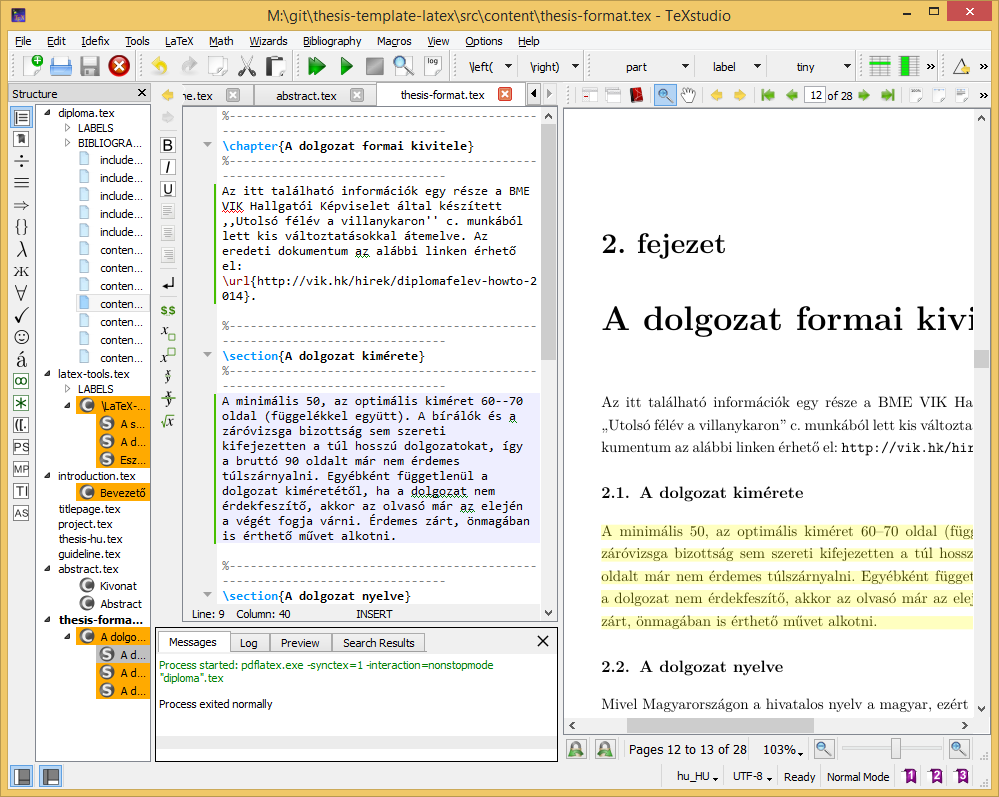
\includegraphics[width=67mm, keepaspectratio]{figures/TeXstudio.png}\hspace{1cm}
	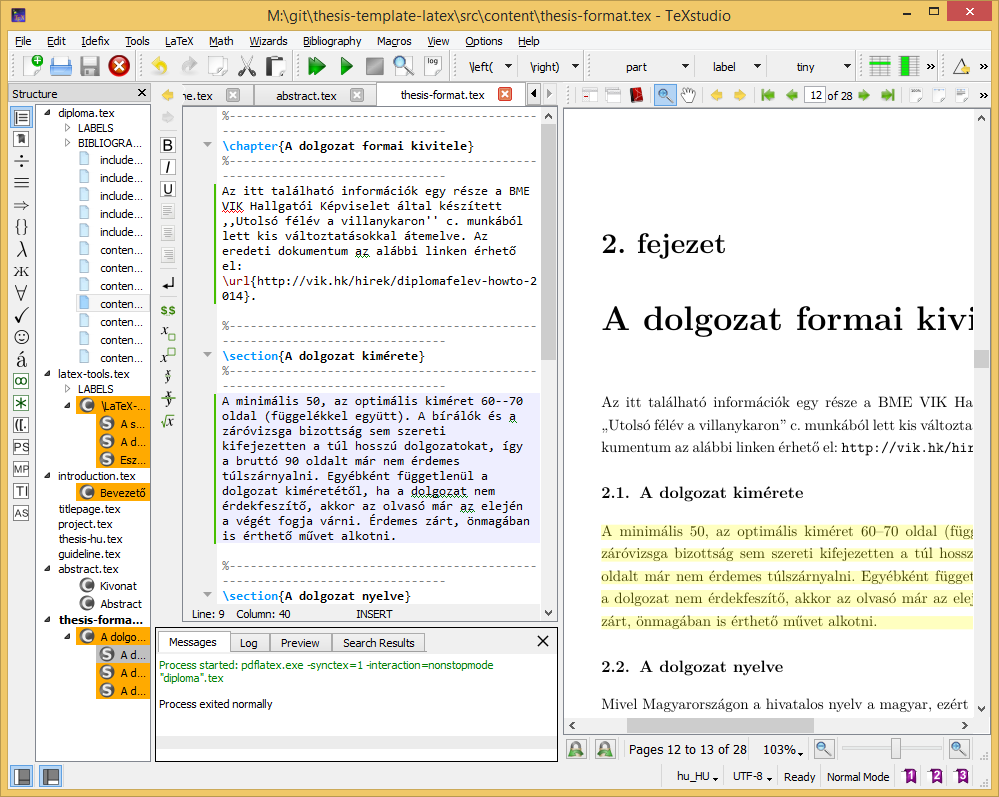
\includegraphics[width=67mm, keepaspectratio]{figures/TeXstudio.png}\\\vspace{5mm}
	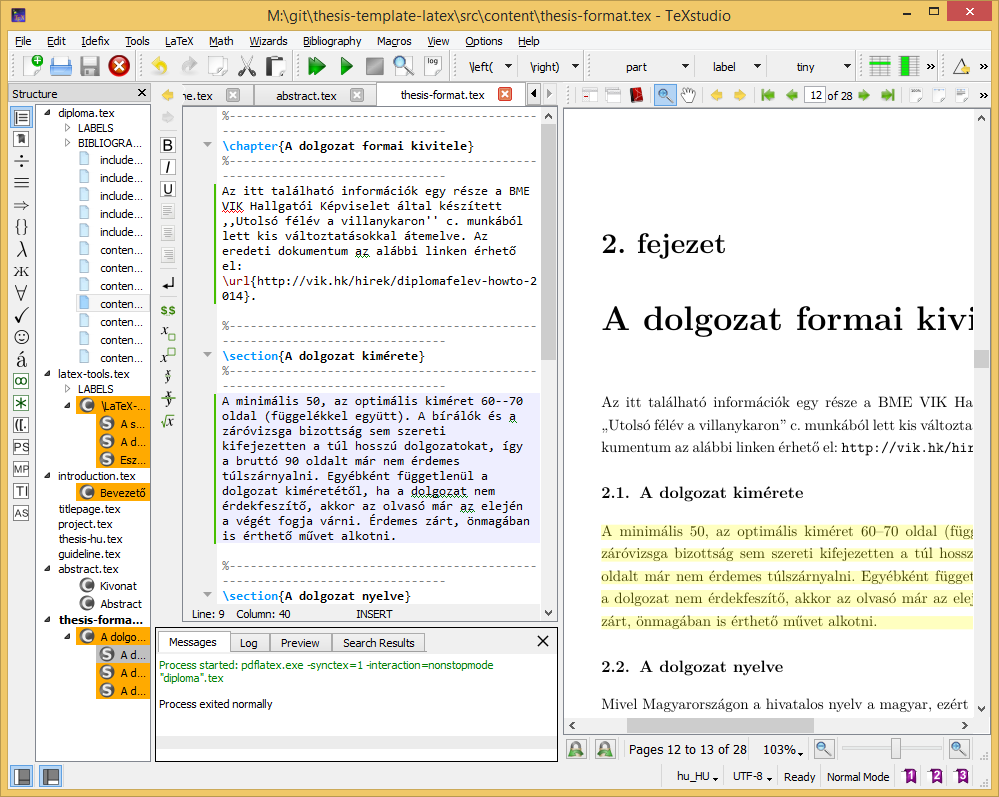
\includegraphics[width=67mm, keepaspectratio]{figures/TeXstudio.png}\hspace{1cm}
	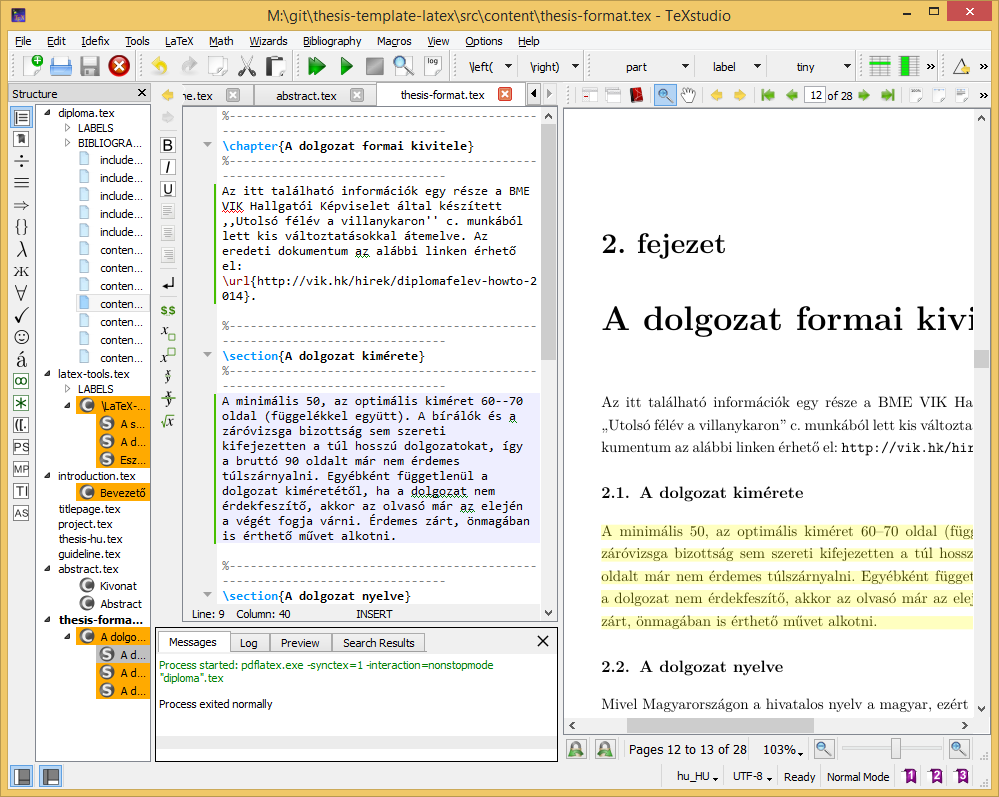
\includegraphics[width=67mm, keepaspectratio]{figures/TeXstudio.png}
	\caption{Több képfájl beillesztése esetén térközöket is érdemes használni.}
	\label{fig:HVSpaces}
\end{figure}

A táblázatok használatára \aref{tab:TabularExample}~táblázat mutat példát. A táblázatok formázásához hasznos tanácsokat találunk a \verb+booktabs+ csomag dokumentációjában.

\begin{table}[ht]
	\footnotesize
	\centering
	\begin{tabular}{ l c c }
		\toprule
		Órajel & Frekvencia & Cél pin \\
		\midrule
		CLKA & 100 MHz & FPGA CLK0\\
		CLKB & 48 MHz  & FPGA CLK1\\
		CLKC & 20 MHz  & Processzor\\
		CLKD & 25 MHz  & Ethernet chip \\
		CLKE & 72 MHz  & FPGA CLK2\\
		XBUF & 20 MHz  & FPGA CLK3\\
		\bottomrule
	\end{tabular}
	\caption{Az órajel-generátor chip órajel-kimenetei.}
	\label{tab:TabularExample}
\end{table}


%----------------------------------------------------------------------------
\section{Felsorolások és listák}
%----------------------------------------------------------------------------
Számozatlan felsorolásra mutat példát a jelenlegi bekezdés:
\begin{itemize}
	\item \emph{első bajusz:} ide lehetne írni az első elem kifejését,
	\item \emph{második bajusz:} ide lehetne írni a második elem kifejését,
	\item \emph{ez meg egy szakáll:} ide lehetne írni a harmadik elem kifejését.
\end{itemize}

Számozott felsorolást is készíthetünk az alábbi módon:
\begin{enumerate}
	\item \emph{első bajusz:} ide lehetne írni az első elem kifejését, és ez a kifejtés így néz ki, ha több sorosra sikeredik,
	\item \emph{második bajusz:} ide lehetne írni a második elem kifejését,
	\item \emph{ez meg egy szakáll:} ide lehetne írni a harmadik elem kifejését.
\end{enumerate}
A felsorolásokban sorok végén vessző, az utolsó sor végén pedig pont a szokásos írásjel. Ez alól kivételt képezhet, ha az egyes elemek több teljes mondatot tartalmaznak.

Listákban a dolgozat szövegétől elkülönítendő kódrészleteket, programsorokat, pszeudo-kódokat jeleníthetünk meg (\ref{lst:Example}.~kódrészlet).
\begin{lstlisting}[language=tex,caption=A fenti számozott felsorolás \LaTeX-forráskódja,label=lst:Example]
\begin{enumerate}
	\item \emph{els(*@ő@*) bajusz:} ide lehetne írni az els(*@ő@*) elem kifejését,
	és ez a kifejtés így néz ki, ha több sorosra sikeredik,
	\item \emph{második bajusz:} ide lehetne írni a második elem kifejését,
	\item \emph{ez meg egy szakáll:} ide lehetne írni a harmadik elem kifejését.
\end{enumerate}
\end{lstlisting}
A lista keretét, háttérszínét, egész stílusát megválaszthatjuk. Ráadásul különféle programnyelveket és a nyelveken belül kulcsszavakat is definiálhatunk, ha szükséges. Erről bővebbet a \verb+listings+ csomag hivatalos leírásában találhatunk.

%----------------------------------------------------------------------------
\section{Képletek}
%----------------------------------------------------------------------------
Ha egy formula nem túlságosan hosszú, és nem akarjuk hivatkozni a szövegből, mint például a $e^{i\pi}+1=0$ képlet, \emph{szövegközi képletként} szokás leírni. Csak, hogy másik példát is lássunk, az $U_i=-d\Phi/dt$ Faraday-törvény a $\rot E=-\frac{dB}{dt}$ differenciális alakban adott Maxwell-egyenlet felületre vett integráljából vezethető le. Látható, hogy a \LaTeX-fordító a sorközöket betartja, így a szöveg szedése esztétikus marad szövegközi képletek használata esetén is.

Képletek esetén az általános konvenció, hogy a kisbetűk skalárt, a kis félkövér betűk ($\mathbf{v}$) oszlopvektort -- és ennek megfelelően $\mathbf{v}^T$ sorvektort -- a kapitális félkövér betűk ($\mathbf{V}$) mátrixot jelölnek. Ha ettől el szeretnénk térni, akkor az alkalmazni kívánt jelölésmódot célszerű külön alfejezetben definiálni. Ennek megfelelően, amennyiben $\mathbf{y}$ jelöli a mérések vektorát, $\mathbf{\vartheta}$ a paraméterek vektorát és $\hat{\mathbf{y}}=\mathbf{X}\vartheta$ a paraméterekben lineáris modellt, akkor a \emph{Least-Squares} értelemben optimális paraméterbecslő $\hat{\mathbf{\vartheta}}_{LS}=(\mathbf{X}^T\mathbf{X})^{-1}\mathbf{X}^T\mathbf{y}$ lesz.

Emellett kiemelt, sorszámozott képleteket is megadhatunk, ennél az \verb+equation+ és a \verb+eqnarray+ környezetek helyett a korszerűbb \verb+align+ környezet alkalmazását javasoljuk (több okból, különféle problémák elkerülése végett, amelyekre most nem térünk ki). Tehát
\begin{align}
\dot{\mathbf{x}}&=\mathbf{A}\mathbf{x}+\mathbf{B}\mathbf{u},\\
\mathbf{y}&=\mathbf{C}\mathbf{x},
\end{align}
ahol $\mathbf{x}$ az állapotvektor, $\mathbf{y}$ a mérések vektora és $\mathbf{A}$, $\mathbf{B}$ és $\mathbf{C}$ a rendszert leíró paramétermátrixok. Figyeljük meg, hogy a két egyenletben az egyenlőségjelek egymáshoz igazítva jelennek meg, mivel a mindkettőt az \& karakter előzi meg a kódban. Lehetőség van számozatlan kiemelt képlet használatára is, például
\begin{align}
\dot{\mathbf{x}}&=\mathbf{A}\mathbf{x}+\mathbf{B}\mathbf{u},\nonumber\\
\mathbf{y}&=\mathbf{C}\mathbf{x}\nonumber.
\end{align}
Mátrixok felírására az $\mathbf{A}\mathbf{x}=\mathbf{b}$ inhomogén lineáris egyenlet részletes kifejtésével mutatunk példát:
\begin{align}
\begin{bmatrix}
a_{11} & a_{12} & \dots & a_{1n}\\
a_{21} & a_{22} & \dots & a_{2n}\\
\vdots & \vdots & \ddots & \vdots\\
a_{m1} & a_{m2} & \dots & a_{mn}
\end{bmatrix}
\begin{pmatrix}x_1\\x_2\\\vdots\\x_n\end{pmatrix}=
\begin{pmatrix}b_1\\b_2\\\vdots\\b_m\end{pmatrix}.
\end{align}
A \verb+\frac+ utasítás hatékonyságát egy általános másodfokú tag átviteli függvényén keresztül mutatjuk be, azaz
\begin{align}
W(s)=\frac{A}{1+2T\xi s+s^2T^2}.
\end{align}
A matematikai mód minden szimbólumának és képességének a bemutatására természetesen itt nincs lehetőség, de gyors referenciaként hatékonyan használhatók a következő linkek:\\
\indent\url{http://www.artofproblemsolving.com/LaTeX/AoPS_L_GuideSym.php},\\
\indent\url{http://www.ctan.org/tex-archive/info/symbols/comprehensive/symbols-a4.pdf},\\
\indent\url{ftp://ftp.ams.org/pub/tex/doc/amsmath/short-math-guide.pdf}.\\
Ez pedig itt egy magyarázat, hogy miért érdemes \verb+align+ környezetet használni:\\
\indent\url{http://texblog.net/latex-archive/maths/eqnarray-align-environment/}.

%----------------------------------------------------------------------------
\section{Irodalmi hivatkozások}
\label{sec:HowtoReference}
%----------------------------------------------------------------------------
Egy \LaTeX~dokumentumban az irodalmi hivatkozások definíciójának két módja van. Az egyik a \verb+\thebibliograhy+ környezet használata a dokumentum végén, az \verb+\end{document}+ lezárás előtt.
\begin{lstlisting}[language=tex]
\begin{thebibliography}{9}

\bibitem{Lamport94} Leslie Lamport, \emph{\LaTeX: A Document Preparation System}.
Addison Wesley, Massachusetts, 2nd Edition, 1994.

\end{thebibliography}
\end{lstlisting}

Ezek után a dokumentumban a \verb+\cite{Lamport94}+ utasítással hivatkozhatunk a forrásra. A fenti megadás viszonylag kötetlen, a szerző maga formázza az irodalomjegyzéket (ami gyakran inkonzisztens eredményhez vezet).

Egy sokkal professzionálisabb módszer a BiB\TeX{} használata, ezért ez a sablon is ezt támogatja. Ebben az esetben egy külön szöveges adatbázisban definiáljuk a forrásmunkákat, és egy külön stílusfájl határozza meg az irodalomjegyzék kinézetét. Ez, összhangban azzal, hogy külön formátumkonvenció határozza meg a folyóirat-, a könyv-, a konferenciacikk- stb. hivatkozások kinézetét az irodalomjegyzékben (a sablon használata esetén ezzel nem is kell foglalkoznia a hallgatónak, de az eredményt célszerű ellenőrizni). felhasznált hivatkozások adatbázisa egy \verb+.bib+ kiterjesztésű szöveges fájl, amelynek szerkezetét a \Aref{lst:Bibtex} kódrészlet demonstrálja. A forrásmunkák bevitelekor a sor végi vesszők külön figyelmet igényelnek, mert hiányuk a BiB\TeX-fordító hibaüzenetét eredményezi. A forrásmunkákat típus szerinti kulcsszó vezeti be (\verb+@book+ könyv, \verb+@inproceedings+ konferenciakiadványban megjelent cikk, \verb+@article+ folyóiratban megjelent cikk, \verb+@techreport+ valamelyik egyetem gondozásában megjelent műszaki tanulmány, \verb+@manual+ műszaki dokumentáció esetén stb.). Nemcsak a megjelenés stílusa, de a kötelezően megadandó mezők is típusról-típusra változnak. Egy jól használható referencia a \url{http://en.wikipedia.org/wiki/BibTeX} oldalon található.

\begin{lstlisting}[caption=Példa szöveges irodalomjegyzék-adatbázisra Bib\TeX{} használata esetén.,label=lst:Bibtex]
@book{Wettl04,
  author    = {Ferenc Wettl and Gyula Mayer and Péter Szabó},
  publisher = {Panem Könyvkiadó},
  title     = {\LaTeX~kézikönyv},
  year      = {2004},
}

@article{Candy86,
  author       = {James C. Candy},
  journaltitle = {{IEEE} Trans.\ on Communications},
  month        = {01},
  note         = {\doi{10.1109/TCOM.1986.1096432}},
  number       = {1},
  pages        = {72--76},
  title        = {Decimation for Sigma Delta Modulation},
  volume       = {34},
  year         = {1986},
}

@inproceedings{Lee87,
  author    = {Wai L. Lee and Charles G. Sodini},
  booktitle = {Proc.\ of the IEEE International Symposium on Circuits and Systems},
  location  = {Philadelphia, PA, USA},
  month     = {05~4--7},
  pages     = {459--462},
  title     = {A Topology for Higher Order Interpolative Coders},
  vol       = {2},
  year      = {1987},
}

@thesis{KissPhD,
  author      = {Peter Kiss},
  institution = {Technical University of Timi\c{s}oara, Romania},
  month       = {04},
  title       = {Adaptive Digital Compensation of Analog Circuit Imperfections for Cascaded Delta-Sigma Analog-to-Digital Converters},
  type        = {phdthesis},
  year        = {2000},
}

@manual{Schreier00,
  author       = {Richard Schreier},
  month        = {01},
  note         = {\url{http://www.mathworks.com/matlabcentral/fileexchange/}},
  organization = {Oregon State University},
  title        = {The Delta-Sigma Toolbox v5.2},
  year         = {2000},
}

@misc{DipPortal,
  author       = {{Budapesti Műszaki és Gazdaságtudományi Egyetem Villamosmérnöki és Informatikai Kar}},
  howpublished = {\url{http://diplomaterv.vik.bme.hu/}},
  title        = {Diplomaterv portál (2011. február 26.)},
}

@incollection{Mkrtychev:1997,
  author    = {Mkrtychev, Alexey},
  booktitle = {Logical Foundations of Computer Science},
  doi       = {10.1007/3-540-63045-7_27},
  editor    = {Adian, Sergei and Nerode, Anil},
  isbn      = {978-3-540-63045-6},
  pages     = {266-275},
  publisher = {Springer Berlin Heidelberg},
  series    = {Lecture Notes in Computer Science},
  title     = {Models for the logic of proofs},
  url       = {http://dx.doi.org/10.1007/3-540-63045-7_27},
  volume    = {1234},
  year      = {1997},
}
\end{lstlisting}

A stílusfájl egy \verb+.sty+ kiterjesztésű fájl, de ezzel lényegében nem kell foglalkozni, mert vannak beépített stílusok, amelyek jól használhatók. Ez a sablon a BiB\TeX-et használja, a hozzá tartozó adatbázisfájl a \verb+mybib.bib+ fájl. Megfigyelhető, hogy az irodalomjegyzéket a dokumentum végére (a \verb+\end{document}+ utasítás elé) beillesztett \verb+\bibliography{mybib}+ utasítással hozhatjuk létre, a stílusát pedig ugyanitt a  \verb+\bibliographystyle{plain}+ utasítással adhatjuk meg. Ebben az esetben a \verb+plain+ előre definiált stílust használjuk (a sablonban is ezt állítottuk be). A \verb+plain+ stíluson kívül természetesen számtalan más előre definiált stílus is létezik. Mivel a \verb+.bib+ adatbázisban ezeket megadtuk, a BiB\TeX-fordító is meg tudja különböztetni a szerzőt a címtől és a kiadótól, és ez alapján automatikusan generálódik az irodalomjegyzék a stílusfájl által meghatározott stílusban.

Az egyes forrásmunkákra a szövegből továbbra is a \verb+\cite+ paranccsal tudunk hivatkozni, így \aref{lst:Bibtex}.~kódrészlet esetén a hivatkozások rendre \verb+\cite{Wettl04}+, \verb+\cite{Candy86}+, \verb+\cite{Lee87}+, \verb+\cite{KissPhD}+, \verb+\cite{Schreirer00}+,
\verb+\cite{Mkrtychev:1997}+ és \verb+\cite{DipPortal}+. Az egyes forrásmunkák sorszáma az irodalomjegyzék bővítésekor változhat. Amennyiben az aktuális számhoz illeszkedő névelőt szeretnénk használni, használjuk az \verb+\acite{}+ parancsot.

Az irodalomjegyzékben alapértelmezésben csak azok a forrásmunkák jelennek meg, amelyekre található hivatkozás a szövegben, és ez így alapvetően helyes is, hiszen olyan forrásmunkákat nem illik az irodalomjegyzékbe írni, amelyekre nincs hivatkozás.

Mivel a fordítási folyamat során több lépésben oldódnak fel a szimbólumok, ezért gyakran többször is le kell fordítani a dokumentumot. Ilyenkor ez első 1-2 fordítás esetleg szimbólum-feloldásra vonatkozó figyelmeztető üzenettel zárul. Ha hibaüzenettel zárul bármelyik fordítás, akkor nincs értelme megismételni, hanem a hibát kell megkeresni. A \verb+.bib+ fájl megváltoztatáskor sokszor nincs hatása a változtatásnak azonnal, mivel nem mindig fut újra a BibTeX fordító. Ezért célszerű a változtatás után azt manuálisan is lefuttatni (TeXstudio esetén \verb+Tools/Bibliography+).

Hogy a szövegbe ágyazott hivatkozások kinézetét demonstráljuk, itt most sorban meghivatkozzuk a \cite{Wettl04}, \cite{Candy86}, \cite{Lee87}, \cite{KissPhD}, \cite{Schreier00} és \acite{Mkrtychev:1997}\footnote{Informatikai témában gyakran hivatkozunk cikkeket a Springer LNCS valamely kötetéből, ez a hivatkozás erre mutat egy helyes példát.} forrásmunkát, valamint \acite{DipPortal} weboldalt.

Megjegyzendő, hogy az ékezetes magyar betűket is tartalmazó \verb+.bib+ fájl az \verb+inputenc+ csomaggal betöltött \verb+latin2+ betűkészlet miatt fordítható. Ugyanez a \verb+.bib+ fájl hibaüzenettel fordul egy olyan dokumentumban, ami nem tartalmazza a \verb+\usepackage[latin2]{inputenc}+ sort. Speciális igény esetén az irodalmi adatbázis általánosabb érvényűvé tehető, ha az ékezetes betűket speciális latex karakterekkel helyettesítjük a \verb+.bib+ fájlban, pl. á helyett \verb+\'{a}+-t vagy ő helyett \verb+\H{o}+-t írunk.

Irodalomhivatkozásokat célszerű először olyan szolgáltatásokban keresni, ahol jó minőségű bejegyzések találhatók (pl. ACM Digital Library,\footnote{\url{https://dl.acm.org/}} DBLP,\footnote{\url{http://dblp.uni-trier.de/}} IEEE Xplore,\footnote{\url{http://ieeexplore.ieee.org/}} SpringerLink\footnote{\url{https://link.springer.com/}}) és csak ezek után használni kevésbé válogatott forrásokat (pl. Google Scholar\footnote{\url{http://scholar.google.com/}}). A jó minőségű bejegyzéseket is érdemes megfelelően tisztítani.\footnote{\url{https://github.com/FTSRG/cheat-sheets/wiki/BibTeX-Fixing-entries-from-common-sources}} A sablon angol nyelvű változatában használt \texttt{plainnat} beállítás egyik sajátossága, hogy a cikkhez generált hivatkozás a cikk DOI-ját és URL-jét is tartalmazza, ami gyakran duplikátumhoz vezet -- érdemes tehát a DOI-kat tartalmazó URL mezőket törölni. 

%----------------------------------------------------------------------------
\section{A dolgozat szerkezete és a forrásfájlok}
%----------------------------------------------------------------------------
A diplomatervsablonban a TeX fájlok két alkönyvtárban helyezkednek el. Az \verb+include+ könyvtárban azok szerepelnek, amiket tipikusan nem kell szerkesztenünk, ezek a sablon részei (pl. címoldal). A \verb+content+ alkönyvtárban pedig a saját munkánkat helyezhetjük el. Itt érdemes az egyes fejezeteket külön \TeX{} állományokba rakni.

A diplomatervsablon (a kari irányelvek szerint) az alábbi fő fejezetekből áll:
\begin{enumerate}
	\item 1 oldalas \emph{tájékoztató} a szakdolgozat/diplomaterv szerkezetéről (\verb+include/guideline.tex+), ami a végső dolgozatból törlendő,
	\item \emph{feladatkiírás} (\verb+include/project.tex+), a dolgozat nyomtatott verzójában ennek a helyére kerül a tanszék által kiadott, a tanszékvezető által aláírt feladatkiírás, a dolgozat elektronikus verziójába pedig a feladatkiírás egyáltalán ne kerüljön bele, azt külön tölti fel a tanszék a diplomaterv-honlapra,
	\item \emph{címoldal} (\verb+include/titlepage.tex+),
	\item \emph{tartalomjegyzék} (\verb+thesis.tex+),
	\item a diplomatervező \emph{nyilatkozat}a az önálló munkáról (\verb+include/declaration.tex+),
	\item 1-2 oldalas tartalmi \emph{összefoglaló} magyarul és angolul, illetve elkészíthető még további nyelveken is (\verb+content/abstract.tex+),
	\item \emph{bevezetés}: a feladat értelmezése, a tervezés célja, a feladat indokoltsága, a diplomaterv felépítésének rövid összefoglalása (\verb+content/introduction.tex+),
	\item sorszámmal ellátott \emph{fejezetek}: a feladatkiírás pontosítása és részletes elemzése, előzmények (irodalomkutatás, hasonló alkotások), az ezekből levonható következtetések, a tervezés részletes leírása, a döntési lehetőségek értékelése és a választott megoldások indoklása, a megtervezett műszaki alkotás értékelése, kritikai elemzése, továbbfejlesztési lehetőségek,
	\item esetleges \emph{köszönetnyilvánítás}ok (\verb+content/acknowledgement.tex+),
	\item részletes és pontos \emph{irodalomjegyzék} (ez a sablon esetében automatikusan generálódik a \verb+thesis.tex+ fájlban elhelyezett \verb+\bibliography+ utasítás hatására, \az+\refstruc{sec:HowtoReference}ban leírtak szerint),
	\item \emph{függelékek} (\verb+content/appendices.tex+).
\end{enumerate}

A sablonban a fejezetek a \verb+thesis.tex+ fájlba vannak beillesztve \verb+\include+ utasítások segítségével. Lehetőség van arra, hogy csak az éppen szerkesztés alatt álló \verb+.tex+ fájlt fordítsuk le, ezzel lerövidítve a fordítási folyamatot. Ezt a lehetőséget az alábbi kódrészlet biztosítja a \verb+thesis.tex+ fájlban.
\begin{lstlisting}
\includeonly{
	guideline,%
	project,%
	titlepage,%
	declaration,%
	abstract,%
	introduction,%
	chapter1,%
	chapter2,%
	chapter3,%
	acknowledgement,%
	appendices,%
}
\end{lstlisting}

Ha az alábbi kódrészletben az egyes sorokat a \verb+%+ szimbólummal kikommentezzük, akkor a megfelelő \verb+.tex+ fájl nem fordul le. Az oldalszámok és a tartalomjegyék természetesen csak akkor billennek helyre, ha a teljes dokumentumot lefordítjuk.

%----------------------------------------------------------------------------
\newpage
\section{Alapadatok megadása}
%----------------------------------------------------------------------------
A diplomaterv alapadatait (cím, szerző, konzulens, konzulens titulusa) a \verb+thesis.tex+ fájlban lehet megadni.

%----------------------------------------------------------------------------
\section{Új fejezet írása}
%----------------------------------------------------------------------------
A főfejezetek külön \verb+content+ könyvtárban foglalnak helyet. A sablonhoz 3 fejezet készült. További főfejezeteket úgy hozhatunk létre, ha új \TeX~fájlt készítünk a fejezet számára, és a \verb+thesis.tex+ fájlban, a \verb+\include+ és \verb+\includeonly+ utasítások argumentumába felvesszük az új \verb+.tex+ fájl nevét.


%----------------------------------------------------------------------------
\section{Definíciók, tételek, példák}
%----------------------------------------------------------------------------

\begin{definition}[Fluxuskondenzátor térerőssége]
Lorem ipsum dolor sit amet, consectetur adipiscing elit, sed do eiusmod tempor incididunt ut labore et dolore magna aliqua. Ut enim ad minim veniam, quis nostrud exercitation ullamco laboris nisi ut aliquip ex ea commodo consequat.
\end{definition}

\begin{example}
Példa egy példára. Duis aute irure dolor in reprehenderit in voluptate velit esse cillum dolore eu fugiat nulla pariatur. Excepteur sint occaecat cupidatat non proident, sunt in culpa qui officia deserunt mollit anim id est laborum.
\end{example}

\begin{theorem}[Kovács tétele]
Duis aute irure dolor in reprehenderit in voluptate velit esse cillum dolore eu fugiat nulla pariatur. Excepteur sint occaecat cupidatat non proident, sunt in culpa qui officia deserunt mollit anim id est laborum.
\end{theorem}

\chapter{Bevezetés}

Konzulensem, Dr. Szegletes Luca már régóta gyűjt videokártyás kódimplementációkat különböző NP-nehéz problémákra. Amikor megbeszéltük, hogy mi lenne a munkám célja, különböző útkeresési algoritmusok megvalósítását kaptam feladatul. A járműútvonal-tervezési algoritmusoknak nagyon sok alesete van, ugyanis végtelenül sokféle feltételt szabhatunk meg egy bejárás számára: a teljes hossz legyen rövid, az egyes utak legyenek egyenként rövidek, stb. Különböző alkalmazásokhoz nagyon változatos elvárások illenek: például ha egy bútor szállítmányozási cég akarja megtervezni, hogy az aznapi 20 klienséhez milyen sorrendben juttassa el az árukat, már azt is bele kell kalkulálnia, hogy hogyan fognak a termékek elférni egy kamionban (véges kapacitás problémája). Másik példa egy nemzetközi körutazás: a cég vezérigazgatója be szeretné járni egy kampány keretében a cég különböző leányvállalatait, melyek manapság a világ bármely pontján lehetnek: lehet, hogy az egyik üzem Kolumbia közepén, míg egy másik valahol Indiában van. A két ország időzónája nagyon különböző, ezért nem mindegy, hogy az igazgató a nap melyik órájában szeretne találkozni a helyi vezetőkkel (a kliens nem áll korlátlanul rendelkezésre, igazítani kell a fogadó és vendég beosztását). Számtalan hasonló szituáció képzelhető el, a fent említettek csak a legtipikusabbak. Ezen problémákat a számítástudomány már évtizedek óta aktívan kutatja. 

\begin{figure}[ht!]
	\centering
	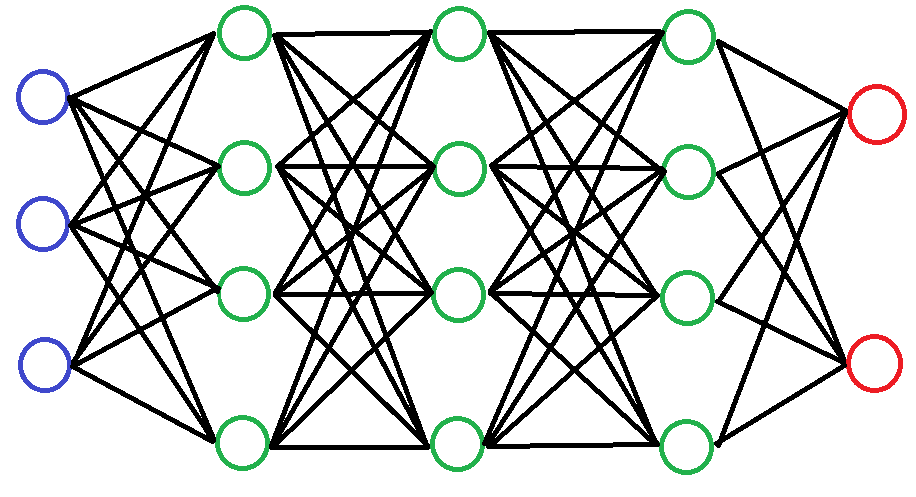
\includegraphics[width=150mm, keepaspectratio]{figures/neurons.png}
	\caption{Többféle modellt is kitaláltak már gépi tanuláshoz, az egyik leghíresebb az ún. neuronháló modell }
\end{figure}
Napjainkban a mesterséges intelligencia forradalmasította a számítástechnikát a számítási kapacitások soha eddig nem látott bővülése eredményeképpen. Az NVIDIA egy olyan cég, amely hardvergyártóként, videokártyák gyártásával és értékesítésével kezdte működését. Az elmúlt években komoly szerkezetváltozáson ment keresztül, igyekszik némileg közönséget is váltani: korábban a videokártyák legnagyobb felvevőpiaca a videojátékosok voltak. A GPU arra lett kitalálva, hogy különböző 2D-, 3D-s renderelési feladatokban tehermentesítse a CPU-t. Több ezer (fizikai) szálon képes futni. Egy GPU szál ezzel szemben sokkal szűkebb utasításkészleten tud dolgozni, mint egy CPU szál. A GPU szálak elsősorban különböző aritmetikai utasítások végrehajtásában jeleskednek: rendelkeznek hardveres FPU-val (floating point unit - olyan hardver, mely lebegőpontos számokon végzett aritmetikára lett tervezve). 
A mesterséges intelligenciát használó algoritmusok azért lettek forradalmi vívmányok, mert az algoritmus kiötletelésének nehézségeit nagyrészt képes kivenni a programozók kezéből. Egy klasszikus módon megírt program írása során a kódírónak teljes körű elképzelése kell, hogy legyen arról, hogy hogyan fog eljutni az eredményhez. 



\begin{figure}[ht!]
	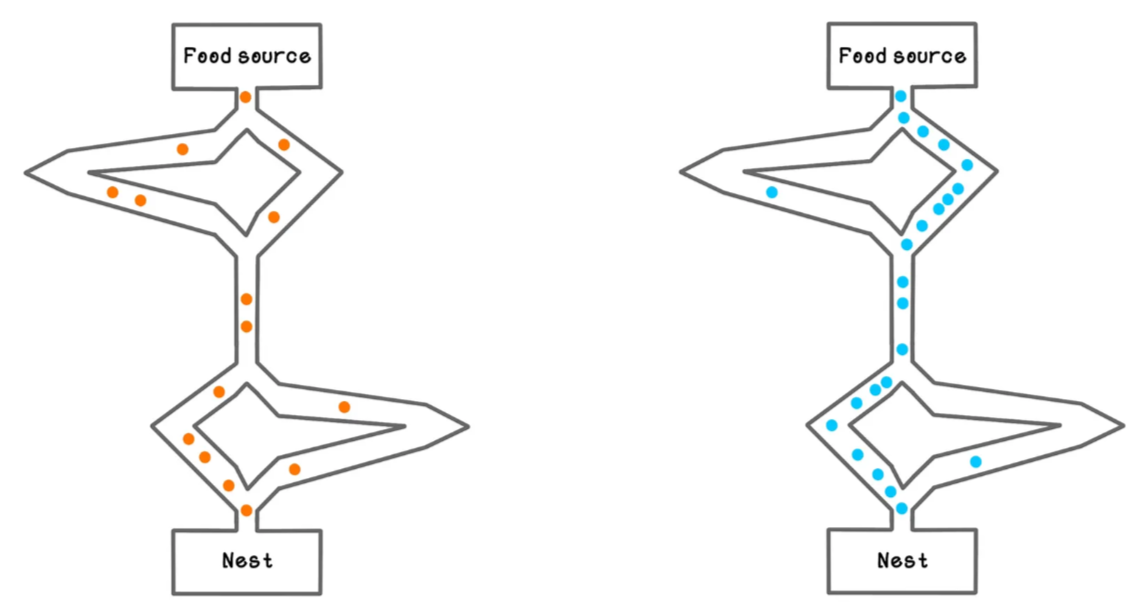
\includegraphics[width=150mm, keepaspectratio]{figures/aco-visualization.png}
	\caption{A hangyák sajátos módon optimalizálják a táplálékszerzést: a Hangyakolónia Optimalizáció segítségével \cite{ACOimage} \label{ACOvisulabel}}
\end{figure}
A gépi tanulás másképp működik: az én esetemben, a \textbf{genetikus algoritmusoknál} kell hozzá egy input, és egy hibafüggvény. A programozó megadja, hogy mely bemenetre szeretné ráengedni az algoritmust. Az algoritmus kap még egy kiértékelő függvényt, amellyel számszerű eredményt rendelhet az általa alkotott megoldásokhoz. A gépnek van memóriaterülete, amelyet az alapján írhat, hogy mit tanult. A genetikus algoritmusok megoldásgenerációkat hoznak létre. A gép a hibafüggvény segítségével értékeli az egyes genomokat, majd a legjobban sikerült egyedek alapján készít következő generációt. A folyamat többféle módon is véget érhet:
\begin{itemize}
	\item a hibafüggvény egy adott hibahatáron belüli megoldást talál
	\item az algoritmus adott ideig (pl. 2 óra) fut, a végső megoldás az utolsó generáció legjobb megoldása
	\item a program adott számú iterációt hajt végre, a végső megoldást készítheti külön, a korábban tanultak alapján
\end{itemize}

A gép kiveszi a programozó kezéből az algoritmizálási feladatot. A kódoló választ egy modellt, amely alapján a gép majd dolgozik. Ha elégedetlenek vagyunk, választhatunk másik modellt, hátha az sikeresebbnek bizonyul.

Szakdolgozatom során a \textbf{Hangyakolónia optimalizáció} modelljét alkalmaztam. Ez egy természetből ellesett trükkön alapuló gráfbejárási algoritmus, a hangyák élelemkeresési módszereire hasonlít, melyet a \ref{ACOvisulabel}. ábra szemlélet.

A koncepció központi elemei a \textbf{feromonok}, melyek biokommunikációra szolgáló, különböző állatok, rovarok által kibocsátott kémiai anyagok, amelyek a faj másik egyedéből meghatározott viselkedést váltanak ki.

A hangyák egész nap a hangyaboly környékét járják morzsák, elhullott rovarok után kutatva. Amikor egy dolgozó korábban felfedezetlen élelemforrást talál, kis részével visszaindul a bolyba, és a hazaúton egyfajta testnedvet, \textbf{feromont} bocsát ki magából. A többi hangya megérzi a szagot, és a nyomába ered. Ha tényleg táplálékhoz vezetett a feromoncsík, akkor ők is kis részével visszaindulnak az élőhelyükre. A folyamat egészen addig tart, amíg van mit elvinni. Ezután az utólag érkező hangyák azt tapasztalják, hogy elfogyott a táplálék, ezért a visszaúton nem választanak ki feromont. A szél előbb-utóbb elfújja az úton hagyott kémiai anyagokat, ezért nem megy oda több egyed.

\section{Fejezetek}
Bevezetés után a \ref{theoryChapter}. fejezetben először ismertetem a problémák elméleti hátterét. Matematikailag kimondom a feladatokat, valamint bemutatom, milyen - főleg valószínűségszámítási - alapok szükségesek a Hangyakolónia optimalizáció alapos megértéséhez.

A \ref{technologyChapter}. fejezetben bemutatom a GPU programozás technológiai hátterét. Kimondom a GPGPU fogalmát. Példákon keresztül szemléltetem a CUDA szoftvermodell markánsabb fogalmait. Különbséget teszek az egyes szinkronizálási szintek között. Ezek után lépésenként megmutatom, hogyan kell Visual Studio segítségével CUDA programot írni és futtatni.

A \ref{implementationChapter}. fejezetben a kódimplementációimat veszem górcső alá. Részletesen beszámolok az egyes logikai elemek működéséről. Bemutatom a Hangyakolónia Algoritmus megjelenését, és az attól való bizonyos eltéréseket. Részletezem a feromonok nyilvántartását, és a véletlen számok kezelését. Logikailag egymásra építem az algoritmusokat ilyen sorrendben: TSP, VRP, CVRP, CVRPTW.

A \ref{resultsChapter}. fejezet a mérési eredményeimet tartalmazza táblázatos formában. Igyekeztem minél szélesebb körben lemérni az egyes adathalmazokat. 

A \ref{results_section}. fejezetben röviden értékelem a kapott eredményeket grafikonokkal szemléltetve. 

\section{Rövidítések}
Dolgozatomban az alábbi rövidítéseket használom:
\begin{itemize}
	\item ACO - Ant Colony Optimization: Hangyakolónia optimalizáció/algoritmus
	
	\item CPU - Processzor
	\item CUDA - Compute Unified Device Architecture
	\item CVRP - Capacitive Vehicle Routing Problem: Korlátozott kapacitású járművek útvonaltervezési problémája
	\item CVRPTW - Capacitive Vehicle Routing Problem with Time Windows: Korlátozott kapacitású, kötött időbeosztású járművek útvonaltervezési problémája
	\item GPU - videokártya
	\item min - minimum
	\item OS - Operating System: Operációs rendszer
	\item PRNG - Pszeudorandomszám-generátor
	\item RAM - Random Access Memory
	\item rep - Repetition: Iteráció
	\item SIMD - Single Instruction Multiple Data
	\item TSP - Travelling Salesman Problem: Utazóügynök probléma
	\item VRP - Vehicle Routing Problems: Járműútvonal-tervezési problémák 
\end{itemize}





\chapter{Elméleti háttér} \label{theoryChapter}

Ahhoz, hogy kellőképpen megértsük a dolgozat által felvetett problémákat, úgy gondolom, hogy szükséges azokat megfelelően, matematikailag tisztán megalapozni. Célom precízen kimondani a megoldandó problémákat, valamint a rájuk alkalmazott különféle technikákat. A témával sokat foglalkozott hallgatótársam, Tóth Márk Andor, munkája számos helyen inspirált \cite{alg_optim}.

\section{Utazóügynök probléma } \label{TSPsection}

Az utazóügynök probléma (Travelling Salesman Problem - TSP)  egy optimalizációs feladat, mely során egy utazónak minél rövidebb úton kell megtennie egy körutat egy adott ponthalmazon. 

Precízen fogalmazva: Adott a bemeneten egy G=(V,E) (irányított) gráf, \[n = |V(G)|, n > 2 \] az állomások száma (a kiindulási állomást beleértve),  \[m = |E(G)| \] az állomások között futó elérhető utak száma.

\[ V = (v_0,v_1, \dots v_n )\] az állomások halmaza (Vertex), \(0 \in V\) a kiindulási állomás,
\[ E = (e_1,e_1, \dots e_m)\] az elérhető utak halmaza (Edge),
\[ D : E(G) \mapsto \mathbb{Z}^+\] az élekhez rendelt költségfüggvény (Distance).

A kimenet a legkisebb költségű Hamilton-kör G-re, vagyis azon 
\[ R = (0, v_{i0}, v_{i1} ... 0) \]
bejárás, amely \( \forall v_i \in V, v_i \in R \) mindegyik csúcsot tartalmazza, és költsége minimális \cite{alg_optim}.

\begin{figure}[ht!]
	\centering
	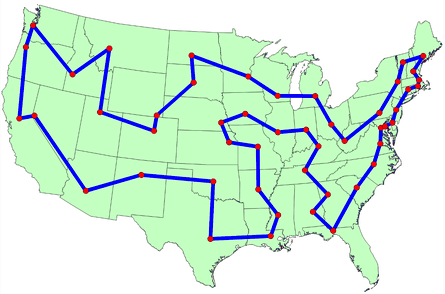
\includegraphics[width=0.5\textwidth]{figures/tsp-usacities.png}
	\caption{Egy példa TSP végrehajtására az USA szárazföldi államai fővárosainak körbeutazása \label{TSPpelda} \cite{TSPimage} }
\end{figure}

A téma a nevét onnan kapta, hogy a XX. században utazó porszívóügynökök autóval járták az Egyesült Államok útjait kereskedés céljából. Az olajválság során megdrágult a járművek működtetéséhez szükséges üzemanyag, és hirtelen megnőtt az igény arra, hogy minél jobban minimalizálják a megtett út hosszát egy-egy üzleti út során. A problémának azóta több alkalmazása is lett, ebből a villamosmérnöki gyakorlathoz egyik legközelebb az SMD beültetőgép bejárása áll. A gép feladata, hogy egy adott nyomtatott áramköri terv alapján lepakolja az alkatrészeket a hordozó lapkára. Az iparban fontos a sebesség, ugyanis ha felére csökkentjük a beültetési időt, akkor akár duplaannyi terméket gyárthatunk le azonos idő alatt. Egy szerelőlemezre alkatrészek százai kerülhetnek, ami nagyon sokféleképpen rendezhető sorba. Természetes igényünk  rövid idő alatt gyors útvonalat találni a beültetőfej számára. A TSP-re \ref{TSPpelda}. ábrán látható egy látványosabb, vizuális szemléltető példa.

\section{Járműútvonal-tervezési problémák \label{VRPsection}}
A járműútvonal-tervezési probléma (Vehicle Routing Problem - VRP) tekinthető a TSP általánosításának. A problémával korábban hallgatótársam, Tóth Márk Andor is foglalkozott, munkája számos helyen inspirált \cite{alg_optim}. A problémát különböző megkötésekkel lehet feltenni az alkalmazás igénye alapján. Ezek lehetnek például:
\begin{itemize}
	\item járművek maximális száma
	\item az egyes járművek szállítási kapacitása
	\item az egyes helyszínekre történő érkezési idő
\end{itemize}

A következőkben feltételezzük, hogy ha több jármű van, akkor azok egy közös kezdőpontból (0. pont, raktár, warehouse) indulnak. Útjuk során minden pontot legalább egyszer érinteniük kell a járműveknek, egyazon csúcsba nem szállíthat csomagot két autó. A \ref{VRPpelda}. ábrán látható egy vizuális szemléltető példa.

\begin{figure}[ht!]
	\centering
	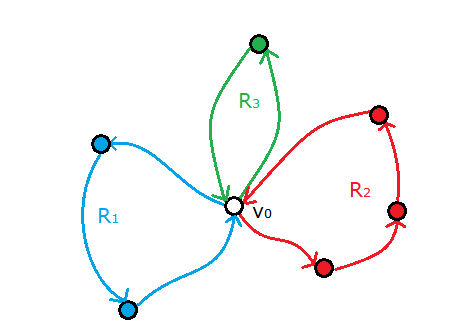
\includegraphics[width=0.5\textwidth]{figures/VRP_Szoveg_nelkul.png}
	\caption{Egy példa VRP végrehajtására n=7 csúcsú gráfon, k=3 járművel \label{VRPpelda} }
\end{figure}

\textbf{Matematikai megfogalmazás :} a problémát gráfokkal modellezhetjük.
\newline 
Legyen \[ G = (V,E) \] (irányított) gráf, n az állomások száma (a kiindulási állomást beleértve), m az állomások között futó elérhető utak száma, k az rendelkezésre álló járművek maximális száma.

\[ V = (v_0,v_1, \dots v_n )\] az állomások halmaza (Vertex), \(0 \in V\) a kiindulási állomás,
\[ E = (e_1,e_1, \dots e_m)\] az elérhető utak halmaza (Edge),
\[ D : E(G) \mapsto \mathbb{Z}^+\] az élekhez rendelt költségfüggvény (Distance),
\[ L = (l_1,l_2, \dots l_k)\] a járművek szállítási kapacitása (Load capacity),
\[ C : V(G)\setminus \{v_0\} \mapsto \mathbb{R}^+ \] az egyes állomások áruigénye (Claim),
\[ T_{min} :  V(G)\setminus \{v_0\} \mapsto \mathbb{R}^+ \] az egyes állomások készenléti ideje,
\[ T_{max} :  V(G)\setminus \{v_0\} \mapsto \mathbb{R}^+ \] az egyes állomások határideje. Értelemszerűen \(T_{max}(v_i) > T_{min}(v_i) \). A járművek sebessége 1 (tetszőleges egység), az idő és távolság egysége ugyanaz.

Az élek azonosítása érdekében éljünk a következő jelöléssel: e\textsubscript{ij} a v\textsubscript{i}-ből v\textsubscript{j}-be mutató él, és d\textsubscript{i,j} az e\textsubscript{i,j} költsége (itt : távolság, distance). Adott továbbá minden csúcshoz a c\textsubscript{i} áruigény, ami ki kell elégíteni (ez a valóságban lehet db, kg, stb.).Adott minden csúcshoz a c\textsubscript{i} áruigény, amit ki kell elégíteni (ez a valóságban lehet darab, kg, stb. ).  Legyen l\textsubscript{i} az i-edik jármű szállítási kapacitása.

Állítsuk elő útvonalak (Route) olyan \( R_{i} = (0, v_{i_1}, v_{i_2}, \dots 0) \) listáit,
ahol az i-edik jármű azon útvonalát adja meg, amelyet alkotó élek 
\( (e_{0,i_{1}}, e_{i_{1},i_{2}}, \dots e_{i_{m},0}) \). Az útvonal költsége az azt alkotó élek összköltsége. 
\begin{equation}
	c(R_i) = \sum_{v \in R_i} c(v)
\end{equation}


A cél azon \(R_1,R_2,...R_k \) útvonalak megtalálása, amelyekre a következők igazak:
\begin{itemize}
	\item összköltségük minimális
	\item kiindulási és végpontjuk a 0. állomás
	\item a kiindulási csúcsot leszámítva minden csúcsot pontosan egyszer tartalmaznak, vagyis \(\forall v_i \in V, v_i\ne v_0\) esetén \( \exists!R_j : v_i \in R_j \). 
	\item egyik jármű sem szállíthat több árut a megengedettnél, vagyis \(l_i \geqslant \sum_{v \in R_i} c(v) \)
	\item a járművek mindegyik állomásra időben megérkeznek: \(\forall v_i \in V, v_i\ne v_0\) esetén \( T_{min}(v_i) \leqslant t(v_i) \leqslant T_{max}(v_i) \)
\end{itemize}


\section{Hangyakolónia optimalizáció}
A \ref{TSPsection}. és \ref{VRPsection}. fejezetekben ismertetett problémákra az optimális megoldás megtalálása NP-nehéz feladat, tehát nagy csúcs- és élhalmaz mellett nem gazdaságos az eredmény kiszámítása. Annak érdekében, hogy a gyakorlatban használható algoritmust konstruáljunk, valamilyen közelítő megoldást érdemes használni a direkt eljárások helyett. A hangyakolónia optimalizáció (Ant Colony Optimization - ACO) egy heurisztikus alapelv, mely gráfbejárások optimalizálásához képes gyorsan, az optimálishoz nagyon közeli megoldásokat találni. Alkalmas a nagyfokú párhuzamosításra, ezért tökéletes választás az NVIDIA\textsuperscript{TM} CUDA architektúrájával történő, GPU alapú adaptálásra.

Az eljárás a nevéből adódóan a hangyák (Formicidae) természetben is megfigyelhető élelemkeresési módszerén alapszik. Az első felfedező hangyák véletlenszerű útvonalakon haladva keresik az élelemhez vezető utat, majd ha sikerrel jártak, akkor a visszaúton feromonnal jelölik meg az útjukat. A többi hangya a szagokat követi, ezért könnyebben, nagy számban tudnak eljutni az elemózsiához. Ha még maradt étel, ők is visszatérve erősítik a feromon nyomokat. Utánpótlás hiányában annak erőssége idővel gyengül, ami modellezhető exponenciális lecsengéssel. Ez természetes módon biztosítja, hogy a nem optimális útvonalak (az élelemhez vezet, de már van nála rövidebb) maguktól elhaljanak. Látható, hogy olyan él, ami sok ideig nem kap feromon utánpótlást, egyre kevesebb hangyát vonz.

Az algoritmus futása során nyilvántartunk egy az eredeti gráf topológiájával megegyező, de eltérő élsúlyozású feromongráfot. Legyen Ph(V,E) gráf, amiben az élek súlyai \( e_{i,j} \rightarrow \tau_{i,j} \) .

Gráfbejárás során egy \(v_i\)-n álló hangya a továbblépéséhez a lehetséges kimenő élek közül a feromon és az élsúly alapján "céltábla elv szerint", véletlenszerűen választ. Úgy kell elképzelni, mintha egy beszínezett darts táblára dobálnánk, és a különböző színekhez az elérhető csúcsok tartoznak, a geometriai valószínűségi mező szerint kisebb-nagyobb valószínűségekkel. Az egyes élek kiválasztásának valószínűsége
\begin{equation}
	P_{i,j} = \frac{(\tau_{i,j})^\alpha(d_{i,j})^\beta}{\sum_{l \in N_i^k}(\tau_{i,l})^\alpha(d_{i,l})^\beta }
	\label{ACO_General_probability}
\end{equation}


ahol \(N_i^k \) az algoritmus k-adik lépésében az i-edik csúcsból elérhető szomszédos csúcsok halmaza. Az \(\alpha\) és \(\beta\) paraméterek a feromonok és élsúlyok figyelembevételét szabályozzák. A cél az, hogy minél nagyobb valahol a feromon, annál inkább akarjunk oda továbbmenni, illetve minél messzebb van egy adott pont, annál inkább el akarjuk kerülni. Jelen esetben elhanyagoltam az élhosszak egyenként külön figyelembe vételét, ezért \(\beta = 0\). Továbbá az egyszerűség kedvéért legyen \(\alpha = 1\). Ennek az lesz az előnye, hogy a \ref{ACO_General_probability}. kifejezés nagymértékben leegyszerűsödik:
\begin{equation}
	P_{i,j} = \frac{\tau_{i,j}}{\sum_{l \in N_i^k}\tau_{i,l}}
	\label{ACO_My_probability}
\end{equation}

Miután minden hangya végigment egy úton (legeneráltunk egy csúcssorrendet, legyen az akár lehetséges, akár nem) értékeljük az útvonalakat. A teljesíthető útvonalak esetén a élek feromonszintjét a útvonal hosszával fordítottan arányosan \(\beta = -1\) megnövelem. Ez biztosítja, hogy a rövidebb útvonalak nagyobb feromonszinttel rendelkezzenek, ezáltal több hangya menjen előbb-utóbb olyan irányba. Valamilyen konstans szorzóra még szükség van a feromonértékek adott tartományba szabályozásához, ezért én még az addíciókat megszorzom a gráfban fellelhető átlagos bejárás hosszával. Így a hangsúly nem a konkrét hosszértékeken, hanem inkább az átlagoshoz vagy az optimálishoz viszonyított arányokon lesz.

Az éleken található feromon növelése után mindegyik élt exponenciális jelleggel csökkentem: minden feromon gyengül egy előre beállítandó, konstans szorzóval, ezzel veszem figyelembe a párolgást (\(\rho\)). Később úgy tapasztaltam, hogy egy \(\rho \approx 0.75\) választás megfelelőnek bizonyult. Tehát az egyes iterációk végén a következő történik egy él feromonjával:
\[ \tau_{i,j} \leftarrow (1-\rho)\tau_{i,j} + \Delta\tau_{i,j} \]

Az útkeresés közben mindig fel kell jegyezni az addig megtalált legjobb utat. Az ACO algoritmus egyik előnye, hogy több, hasonlóan jó alternatív utat is képes megtalálni. Ez például térképes útvonaltervezésnél lehet hasznos. Előfordulhat, hogy valami tőlünk független ok miatt a felhasználó egy objektíven nézve enyhén szuboptimális útvonalat akar inkább. Az eljárás javítása érdekében bevezettem, hogy az a hangya egy ún. "Jutalom szorzó"-t kap, aki minden korábbinál rövidebb utat talál. Ez azzal jár, a feromonjához adandó többlet a sokszorosára, például százszorosára változik, így a következő iterációban sokkal nagyobb valószínűséggel fog arra menni a jövő hangyája. A jutalmazási rendszerem rossz beállítások mellett kezdetben félreviheti a hangyákat egy szuboptimális, de lokálisan minimális útvonal felé. Ha ilyen jelenség tapasztalható, akkor át lehet állítani, hogy hányadik iterációtól kezdve kaphassanak az útvonalak "Jutalom szorzó"-t.

Az eljárás adott számú iteráció után leáll, az eredmény lehetőleg az addig megtalált legrövidebb útvonal. A konkrét implementáció során a \ref{sec:getResult}. fejezetben látni fogjuk, hogy a helyzet bonyolódhat.

\section{Alternatív megoldások}

Dolgozatomban főleg a Hangyakolónia algoritmussal foglalkoztam, de  az nem azt jelenti, hogy ez az egyetlen járható út. Nézzünk meg néhány alternatív megoldási módszert.

\subsection{„Brute force” algoritmus}
A „Brute force” algoritmus lényege, hogy minden lehetséges bejárást megvizsgálunk, és kiválasztjuk a legrövidebb, a konkrét probléma feltétel(rendszer)ének eleget tevő esetet. Magyarul talán "nyers erő" módszerének mondhatnánk, ami kicsit szerencsétlenül hangzik, ezért én a továbbiakban az angol elnevezésével hivatkozok rá. \textbf{Ha n db csúcs}ból álló teljes gráfot nézünk, mint ahogy az a valóságban igen gyakori, \textbf{akkor n! különböző lehetséges bejárás}t kell összehasonlítani. Kis n esetén még csak-csak elfogadható ez a módszer, viszont ha már \(n=48\) db csúcsunk van, mert szeretnénk bejárni TSP szerint az Amerikai Egyesült Államok 48 összefüggő államának fővárosait (később lesz rá példa), a vizsgálandó esetek száma felugrik \( 48! \approx 1.24 * 10^{61} \)-re. Tegyük fel, hogy csúcskategóriás, 5 GHz-en pörgő szuperszámítógépünk képes átlagosan 1 órajelciklusonként (  \(2*10^{-10}s\) időközönként, nagyjából lehetetlenül gyorsan) kiszámolni egy út hosszát, még így is kb. \(2.5 * 10^{51}s \approx 8 * 10^{43} \) évig vizsgálhatnánk az eseteket. Egy SMD beültetőgép a szerelőlemezre akár alkatrészek százait pakolhatja fel, brute force módszerrel lehetetlen lenne megmondani, hogy milyen sorrendben haladjon. Ha szeretnénk véges időn belül megoldani a problémát, akkor ravaszabbnak kell lennünk.

\subsection{Held - Karp algoritmus }
A Held-Karp algoritmust M. Held és R. Karp alkották meg 1962-ben \cite{HeldKarp}. Akkoriban még csak gyerekcipőben a számítástudomány és az informatika, ekkor készültek el az első számítógépek. Módszerük szerint egyesével, rendezetten szúrnak be csúcsokat egy egyre növekvő ponthalmazba. Hasonlít a beillesztéses rendezésre, csak kicsit komplexebb. Kihasználja, hogy a stack (magyarul: verem) és a stackpointer megjelenésével a korai számítógépek is képesek voltak már rekurzív programvégrehajtásra.
\paragraph{}
Jelöljük a csúcsokat \( V=\left(v_1,v_2,\ldots v_n\right) \) -nel, \(v_1\) önkényesen kijelölhető kezdőpont. Legyen S halmaz a csúcsok valamely, a kezdőcsúcsot nem tartalmazó részhalmaza: \(S \subseteq \{v_2,...v_n\}\). Legyen g(S,e) \(v_1\)-ből az S összes elemén keresztül az e \(\neq v_1\)  csúcsban végződő legrövidebb út hossza. Az u-ból a v-be mutató él költsége d(u,v).
Lépésenként kiszámítjuk a g(S,e) értékeket kezdve a kis S-ekre.

Példák:
\begin{itemize}
	\item \(\forall e: g(\emptyset,e) = d(1,e)\)
	\item \(g(\{2\},4)\) csak az összhossza az  \(1 \rightarrowtail 2 \rightarrowtail 4\) útnak
	\item \(g(\{2,3\},4)\)  az ( \(1 \rightarrowtail 2 \rightarrowtail 3 \rightarrowtail 4\) ) és ( \(1 \rightarrowtail 3 \rightarrowtail 2 \rightarrowtail 4\) ) utak rövidebbikének a költsége
\end{itemize}

Amikor már 3 vagy több pontot tartalmaz az S halmaz, a lehetséges utak száma drasztikusan megnő, de egy ügyes trükk felhasználásával csak néhányat kell figyelembe venni a legrövidebb út keresése érdekében. Vegyük észre, hogyha az (\(1\rightarrowtail 4\rightarrowtail 3\rightarrowtail 2\)) út rövidebb, mint az (\(1\rightarrowtail 3\rightarrowtail 4\rightarrowtail 2\)), akkor az (\(1\rightarrowtail 4\rightarrowtail 3\rightarrowtail 2\rightarrowtail 5\)) út is rövidebb lesz, mint a (\(1\rightarrowtail 3\rightarrowtail 4\rightarrowtail 2\rightarrowtail 5\)).
\paragraph{}
Általánosan: tegyük fel, hogy a k-adik lépésben \(S=\{s_1,...s_k\}\). Jelöljük \(1\leqslant i\leqslant k\)-ra \(S_i = S-\{s_i\} = \{s_1...s_{i-1},s_{i+1}...s_k\} \). Ha a \(v_1\)-ből a legrövidebb út e-be S-en keresztül úgy vezet, hogy annak \(s_i\) az utolsó előtti eleme, akkor következik, hogy \(v_1\)-ből a legrövidebb út \(s_i\)-be \(S_i\)-n keresztül vezet. Ez azt jelenti, hogy a k-adik lépésben elég k db S halmazt továbbvinnünk, mert csak azok lehetségesek legrövidebb utat adni.

\subsubsection{Az eljárás Értékelése}
\label{sssec:HeldKarpEvaluate}
A Held-Karp algoritmus exponenciális idejű, \(O(2^nn^2)\), ami nagyságrendekkel jobb, mint a brute-force módszer az ő \(O(n!)\) faktoriális idejével. Előnye a Hangyakolónia algoritmussal szemben, hogy mivel determinisztikus algoritmus, a végén mindig a legrövidebb utat adja eredményül. Komoly hátránya, hogy rekurziót alkalmaz, ami kedvezőtlen a programvégrehajtás szempontjából: sok rekurzív függvényhívás ugyanis megterheli a vermet, sok felesleges másolás történik. Belátható, hogy ha különböző, adott esetekben bonyolult feltételekkel keresünk utakat, akkor az algoritmus elveszíti alapelvét, nem elég mindig az előző ciklus legjobbjaiból kiindulni. Ezzel a problémával az ACO is szembesül, de kevésbé van rá kihatással. Erre még később visszatérek a \ref{section:conditionsWithACO} fejezetben, ahol a feltételek bonyolódásával foglalkozom.

\chapter{Technológiai háttér} \label{technologyChapter}
Ebben a fejezetben szeretném ismertetni a GPU porgramozáshoz felhasznált szoftver- és hardveregyüttest. Először a grafikus segédprocesszoron történő általános célú programozást tárgyalom, majd bemutatom az Nvidia\textsuperscript{TM} által erre kifejlesztett párhuzamos számítási platformot, a CUDA keretrendszert. Részletezem a megértéshez szükséges fontosabb fogalmakat, valamint röviden bemutatom, hogy lehet Visual Studio segítségével CUDA platformon C++ nyelven többszálú programot fejleszteni. A fogalmak összegyűjtéséhez nagymértékben ihletett nyújtott többek között Király Gábor diplomamunkája, mely hasonló témakörrel foglalkozik. \cite{kvantum_optim}

\section{GPGPU}
A GPGPU (general-purpose computing on graphics processing units) egy olyan
szoftverfejlesztési gyakorlat, melynek során a grafikus feldolgozóegységet (GPU) általános
célú számítási műveletek elvégzésére használjuk. \cite{kvantum_optim} Korábban a GPU-t azért találták fel, hogy a grafikus felületek elterjedése után a renderelési, 2D-s vagy 3D-s megjelenítési feladatok terén tehermentesítse a CPU-t. Később kiderült, hogy a GPU alkalmas általánosabb megközelítésekre is, bizonyos aritmetikai utasítások kifejezetten hatékonyan tudnak működni rajta.

\subsection{Motiváció}
Az 1980-as években megjelentek az első személyi számítógépek (PC-k), melyek központi feldolgozóegységei (CPU) kezdetekben néhány MHz-es belső órajellel működtek. Akkor az volt a számítástechnikai fejlesztőmérnökök fő eszköze a számítási gyorsaság növelésére, hogy az órajelfrekvenciát növelték. Ez frekventáltabb utasítás-végrehajtást biztosított, és evidens volt, hogy a nagyobb frekvencia nagyobb számítási erővel is jár. Számos kiváló mérnöki megoldás született, ezek közül talán az egyik legjelentősebb találmány a fáziszárt hurok (Phase-Locked Loop - PLL). A PLL egy olyan Szabályozható hurok, amely (a részleteket mellőzve, nem tárgya dolgozatomnak) egy bemeneti referenciafrekvenciát tud megsokszorozni. Nélküle gyakorlatilag képtelenség lett volna felhasználói szinten 50-60 MHz fölé menni a személyi számítógépek belső órajelénél. Nagyjából 30 évvel később elérték a hardverfejlesztők, hogy a legtöbb asztali processzor órajele 1GHz és 4GHz között legyen képes működni, ez az eredeti PC-k operatív belső frekvenciájának több, mint az ezerszerese. Napjainkban változás látható a fejlesztési trendekben, ugyanis az órajelnövelést a processzorok hődisszipációja felülről korlátozza. Egyelőre nem tűnik könnyen lehetségesnek 5GHz fölé menni úgy, hogy közben az eszköz helyes működése garantálható legyen. A különböző hűtési technológiák (léghűtés, vízhűtés) bizonyos fokig tudnak javítani a sebességen, viszont nagyságrendeket ugrani velük sem lehetséges. 
A számítógépgyártók mai napig új, alternatív megoldásokat keresnek a számítási teljesítmény növelésére. Napjainkban a kutatásoknak két nagy témája van. Egyik a kvantumszámítógépek témaköre, amit dolgozatomban nem részletezek. Másik aktívan vizsgált lehetőség a párhuzamosítás minél több szálon. Már a CPU-k fejlesztésénél is megfigyelhető, hogy inkább a minél több processzormag telepítése az iparági trend.

\begin{figure}[ht!]
	\centering
	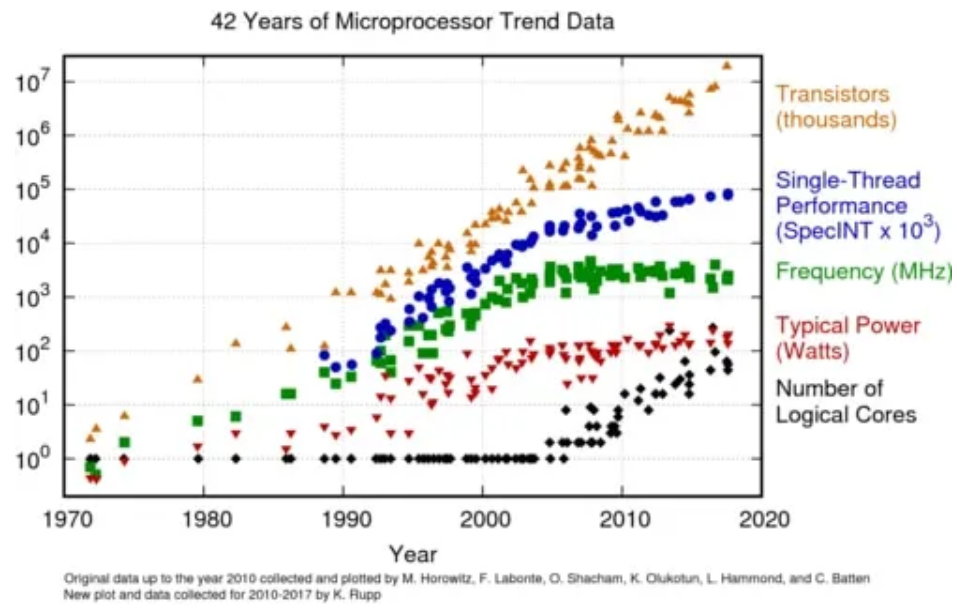
\includegraphics[width=150mm, keepaspectratio]{figures/CPU-cores-trend.png}
	\caption{Látható, hogy kb. 2010-re befejeződött a CPU-k órajelfrekvencia-növekedése, helyette egyre nőni kezdett az egy házon belüli magok száma. \cite{CPUcores} }
\end{figure}

Párhuzamosításra legalkalmasabb a grafikus segédprocesszor, a GPU, hiszen felépítéséből adódóan erre készült. Amíg a CPU feladata az, hogy műveletek egy adott szekvenciáját, és annak minden utasítását a lehető leggyorsabban hajtsa végre, addig a GPU célja minél több szál (akár több ezer, vagy több tízezer) párhuzamos futtatása. A videokártyák előnye akkor válik láthatóvá, ha ugyanazt az utasítást több nagy adattömbön kell végrehajtani. Ez az úgynevezett SIMD megközelítés (Single Instruction Multiple Data). \cite{kvantum_optim}
Az \ref{TransistorsInGpu}. ábra szemlélteti, hogy a CPU-hoz képest a GPU-n arányaiban több tranzisztor van adatfeldolgozásra rendelve, cserébe a gyorsítótárazás és a folyamatvezérlés (feltételkiértékelések, ciklusszervezések) kisebb hangsúlyt kapott.

\begin{figure}[ht!]
	\centering
	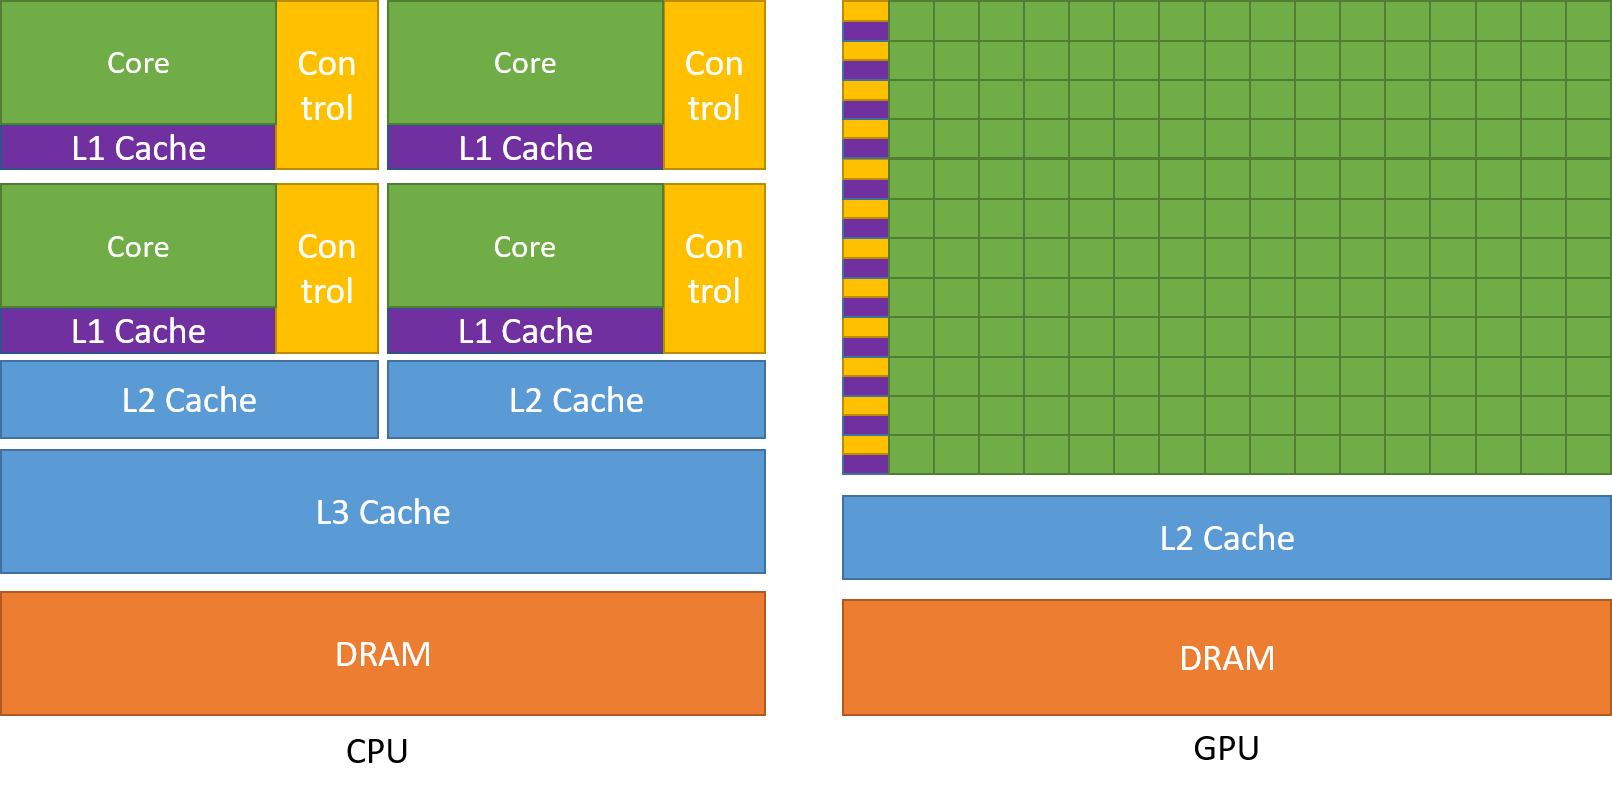
\includegraphics[width=150mm, keepaspectratio] {figures/gpu-devotes-more-transistors-to-data-processing.png}
	\caption{Látható, hogy a gyorsítótárak és a vezérlés rovására nőtt az adatfeldolgozásra szánt tranzisztorok számára. Ez alkalmas lebegőpontos műveletek nagyfokú párhuzamosítására. \cite{CUDAdoc} \label{TransistorsInGpu} }
\end{figure}


A videokártya sokkal nagyobb utasítás-áteresztőképességet, valamint memória-sávszélességet biztosít, mint a CPU hasonló ár és energiafogyasztás mellett. Egyéb számítási eszközök, mint az FPGA-k is lehetnek nagyon energiatakarékosak, viszont azok sokkal kevésbé rugalmasan programozhatóak, mint a GPU-k, ezért a fejlesztési idő sokkal hosszabb lesz és az alkalmazást nehezebb karbantartani. \cite{CUDAdoc}

\section{CUDA}
Többféle keretrendszer is megvalósítja a GPGPU szabta alapelveket. Munkám során a CUDA ( Compute Unified Device Architecture ) rendszerét használtam. A CUDA egy, az NVIDIA által fejlesztett párhuzamos számítási platform és API (felhasználói interfész), amely szoftveres támogatást nyújt az ezzel kompatibilis grafikus feldolgozóegységek általános célú programozására \cite{kvantum_optim}. 

A programozás C vagy C++ nyelven történhet, melyet minimális nyelvi kiegészítésekkel bővítettek, többek között a szálkezelés rendszerszintű használata érdekében. A CUDA programozás tanulásához elérhető egy felettébb kiterjedt dokumentáció a gyártó weboldalán, melyet folyamatosan frissítenek. \cite{CUDAdoc}

\subsection{Programozási modell }
A továbbiakban összefoglalom a legfontosabb fogalmakat úgy, hogy ismertetem, azok hogyan lettek megvalósítva C++ programozási nyelven.

\subsubsection{Kernel, és a többi függvénytípus}
A programozó speciális függvényeket definiálhat, melyeket kernelnek nevezünk. A kernel létesít kapcsolatot a CPU (host) és GPU (device) között. A CPU hívja meg a függvényt, amit aztán a GPU hajt végre, tehát a kernelfüggvény törzse a videokártyán fut végig. Minden egyes kernel példányt egy számára megadott szál hajt végre.
A kernel a "\textit{\_\_global\_\_}" kulcsszóval definiálható. Ezt a függvény fejléce elé kell írni, ettől fogja tudni a szoftverkörnyezet fordítóprogramja, a compiler, hogy mostantól GPU kódként kell értelmezze a programot. Minden, a kernelt végrehajtó szál egy egyedi thread azonosítót kap, mely a beépített threadIdx változón keresztül érhető el a függvényen belül.

Egyéb kulcsszavak is léteznek. Egyik a "\textit{\_\_host\_\_}", ami azt jelzi, hogy CPU által hívott, majd ugyanúgy általa futtatandó kódrészlet következik. Ha nem adunk meg egy függvény elé kulcsszót, akkor azt a preprocesszor host függvénnyé írja át, tiszta CPU kódként értelmezi, mintha nem is lenne a szoftverkörnyezet mögött a CUDA platform. Másik használható jelző a "\textit{\_\_device\_\_}", amely tisztán GPU függvényt jelez. A két kulcsszó vegyíthető: amennyiben azt írjuk, hogy "\textit{\_\_device\_\_ \_\_host\_\_}", a fordító ezt minden egyes híváskor a végrehajtó saját kódjának tekinti, vagyis nem hajt végre vezérlésátadást az eszközök között. Hasznosítható például függvénykönyvtárak GPU-ra kiterjesztésére.

\paragraph{}
Azt, hogy a kernelt felhívásakor hány CUDA szálon szeretnénk futtatni, az új nyelvi elemként megjelenő < < < ··· > > > végrehajtási konfiguráció szintaxissal tudjuk specifikálni. Sajnos a Visual Studio még szintaxishibaként kezeli a mostani, CUDA 12.3 verzióban, ezért a programozónak érdemes odafigyelni, hogy milyen IntelliSense hibaüzeneteket vesz figyelembe. A \ref{invalidErrors}. ábrán például olyan fogalmakra jelez a fejlesztői környezet, amelyek a keretrendszer adta bővítményekben vannak definiálva. 



\begin{figure}[ht!]
	\centering
	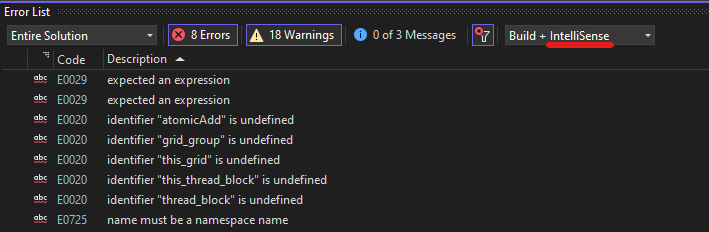
\includegraphics[width=150mm, keepaspectratio] {figures/invalidIntellisenseErrorMessages.png}
	\caption{Bizonyos hibaüzeneteket azért kaphatunk, mert a Visual Studio által használt Intellisense nem ismeri a CUDA nyelvi kiegészítései. Ezeket figyelmen kívül lehet hagyni \label{invalidErrors} }
\end{figure}

\paragraph{Példa:} A hivatalos dokumentáció az alábbi példát adja kernel definícióra. A kódrészlet az N méretű A és B vektorok összeadását végzi és az eredményt a C vektorban tárolja:

\begin{lstlisting}[style=CStyle,showstringspaces=false]
	#define N 1024
	
	// Kernel definition
	__global__ void VecAdd(float* A, float* B, float* C)
	{
		int i = threadIdx.x;
		C[i] = A[i] + B[i];
	}
	
	int main()
	{
		...
		// Kernel invocation with N threads
		VecAdd<<<1, N>>>(A, B, C);
		...
	}
\end{lstlisting}

Megfelelő CPU programkörnyezet hozzáadásával ellenőrizhető, hogy a példában adott kernel tényleg helyes eredményt ad.

\subsubsection{Szálkezelés}
Ahhoz, hogy CUDA programunk megfelelően működjön, az egyes programszálakat rendszereznünk kell. 

Most bemutatom, hogy CUDA API-ban milyen típusú szálak léteznek, és ezeket hogyan lehet különböző szintű szinkronizációkba hozni. Ezen fejezetrészhez intenzíven tanulmányoztam az NVIDIA hivatalos fórumának bejegyzéseit, amit mivel az ott dolgozó fejlesztőmérnökök szerkesztenek, relevánsnak tekintettem. Az egyik leghasznosabb cikket a "Cooperative Groups" nevű bővítményről találtam, a példákat belőle idézem \cite{CUDAcoopgroups}.


Az előző, \ref{secParallelProgramming}. részben láttuk a hatékony párhuzamos program feltételeit. Foglalkozzunk jelen esetben a 3. ponttal, a szinkronizálással. Szinkronizáció szükséges ahhoz, hogy elosztott programunk biztonságos, fenntartható és moduláris legyen. A CUDA 9 bevezette az ún. \textbf{Kooperatív csoport} nevű absztrakciót (angolul Cooperative Groups) \cite{CUDAdoc_coopGroups}, amely erős támogatást nyújt a kerneleknek ahhoz, hogy dinamikusan alakíthassanak ki csoportokat a szálak között.

Korábban a CUDA API egy nagyon egyszerű, de csak speciális esetekben működő megoldást biztosított a szinkronizáció kérdésére, a blokkon belüli "barrier" szinkronizációt: A "\textit{\_\_syncthreads()}" függvény addig nem engedte tovább futni a szálakat, amíg \textbf{a blokkon belül} minden még futó szál el nem jutott az adott pontig. Belátható, hogy nagy szál szám mellett ez nem elég, ugyanis egy blokkon belül jelenlegi GPU-kon legfeljebb 1024 szál futhat. Ha mi több, mint 1024 threadből álló programot írnánk, azaz több Streaming multiprocessor (SM) futna egymással párhuzamosan, akkor ezek összehangolását eddig nem tudtuk volna megfelelő szoftveres támogatással elvégezni. Másik probléma az, hogy ha a szálainknak csak egy kis, adott számú (például 4 vagy 32, de tipikusan 2-hatvány) részhalmazát akarjuk összehangolni akkor korábban azt sem tudtuk szépen megoldani.

A Cooperative Groups egy API Support Package, ami szálak csoportosítását és szinkronizálását segíti CUDA programokban. A Package nagy része az összes CUDA 9-el kompatibilis GPU-ra működik, azaz Kepler és későbbi architektúrákkal (Compute Capability 3.0+) kompatibilis.

Ahhoz, hogy használhassuk a csomagot, be kell illeszteni az alábbi headert .cu vagy .cuh kiterjesztésű fájlunk fejlécébe.

\begin{lstlisting}[style=CStyle]
	#include <cooperative_groups.h>
\end{lstlisting}

A típusok és interfészek a "cooperative\_groups" C++ névtérben vannak definiálva, így mindig prefixként ki kell írjuk, hogy "cooperative\_groups::", vagy betöltjük a névteret a "using" direktívával. Én a munkám során a "using" megoldást választottam.

\begin{lstlisting}[style=CStyle]
	using namespace cooperative_groups; // Névtér betöltése
	using cooperative_groups::thread_group; // stb. 
	namespace cg = cooperative_groups; // Használhatunk rövid aliast is
\end{lstlisting}

\paragraph{Thread csoportok}
Az egyik legfontosabb típus a csomagon belül a "thread\_group" típus, ami threadek, azaz szálak csoportját tudja kezelni. Ezt örökölteti le az összes, később tárgyalandó csoport objektum. A következő alapvető függvények hívhatóak rájuk:

\begin{itemize}
	\item Megkaphatjuk a csoport méretét, azaz a benne futó szálak számát a size() metódussal. Használható túlcímzés elleni védelemre
\end{itemize}	

\begin{lstlisting}[style=CStyle]
	unsigned size();
\end{lstlisting}

\begin{itemize}
	\item Megkaphatjuk a hívó thread indexét (0 és size()-1 közötti) a thread\_rank() metódussal
\end{itemize}	

\begin{lstlisting}[style=CStyle]
	unsigned thread_rank();
\end{lstlisting}

\begin{itemize}	
	\item Megvizsgálhatjuk a csoport érvényességét az is\_valid() függvénnyel
\end{itemize}

\begin{lstlisting}[style=CStyle]
	bool is_valid();
\end{lstlisting}

%TODO kiszedni vagy nem szedni ki?
\paragraph{Thread csoportokon végrahajtható kollektív (egyenhatású) műveletek}

A thread csoportok megadják a lehetőséget, hogy együttesen hajtsunk rajtuk végre műveleteket. Legegyszerűbb operációink egyike a szinkronizálás, ami annyit tesz, hogy a csoport tagjait nem engedi túl egy műveletsoron addig, míg minden tagja el nem jut az adott pontig. Az összes thread csoport fajta támogatja a szinkronizálást, azonban mindegyik kicsit másképp.

Egy adott g csoporthoz tartozó szálakat a kollektív sync() metódussal, vagy g-re a cooperative\_groups::synchronize() függvényt meghívva szinkronizálhatjuk. Ezek a már korábban emlegetett barrier szinkronizációt hajtják végre.
\begin{lstlisting}[style=CStyle]
	g.sync();           // g szinkronizálása
	cg::synchronize(g); // ekvivalens megoldás
\end{lstlisting}

\paragraph{Thread Blokk}
Az első thread csoport fajta a Thread blokk. A Cooperative Groups azért vezette be ezt az adattípust, hogy explicit reprezentálja a CUDA programozás azonos nevű, egyik fontos fogalmát. A szálak egy-, kettő-, vagy háromdimenziós logikai egységbe szervezhetők, amit \textbf{blokk}nak nevezünk. Ez a megoldás egy természetes módot nyújt arra, hogy vektorok vagy mátrixok elemein hajtsunk végre számításokat. 
Az egy blokkba tartozó szálak számát hardveres megfontolások felülről korlátozzák: mivel ezeknek a threadeknek közös processzormagon kell futniuk és a mag korlátos memória-erőforrásain kell osztozniuk, nem foglalhatnak el túl nagy helyet. A jelenlegi GPU-k egy blokkban legfeljebb 1024 thread futtatását támogatják, viszont a kernel több egyenlő méretű blokkban futtatható, ezért a szálak száma megkapható a blokkonkénti szálak száma és a blokkszám szorzataként. \cite{kvantum_optim}
Egy thread blokk példánya az alábbi módon inicializálható:
\begin{lstlisting}[style=CStyle]
	thread_block block = this_thread_block();
\end{lstlisting}

Azon threadek, melyek beépített CUDA blockIdx értékei megegyezőek, ugyanazon thread blokkba tartoznak. A blokkok szinkronizálása nagyon hasonló a korábban emített \_\_syncthreads() metódushoz. A következő kódok mind ugyanolyan hatást érnek el: (feltéve, ha a thread blokk összes szála elér odáig)
\begin{lstlisting}[style=CStyle]
	__syncthreads();
	block.sync();
	cg::synchronize(block);
	this_thread_block().sync();
	cg::synchronize(this_thread_block());
\end{lstlisting}

A "thread\_block" adattípus kiterjeszti a "thread\_group" interfészt két, blokk-specifikus tagfüggvénnyel. Ezek megfeleltethetőek a CUDA API blockIdx és threadIdx tagváltozóinak.
\begin{lstlisting}[style=CStyle]
	dim3 group_index();  // 3-dimenziós blokk index griden belül
	dim3 thread_index(); // 3-dimenziós thread index blokkon belül
\end{lstlisting}


\subsection{Moduláris programszerkesztés}
A kooperatív csoportok használata nem csak gyors, de hasznos is tud lenni. A kódcsomag ereje a modularitás, hogy amikor a csoportot explicit átadjuk függvények között, konzisztensen hivatkozhatunk annak méretére. Ez nehezebbé teszi kritikus versenyhelyzetek, illetve holtpontok kialakulását, mert nem teszünk hibás következtetéseket elágazó függvényhívások között. Az alábbi egy elkerülendő példa hibás szinkronizálásra.
\begin{lstlisting}[style=CStyle]
	__device__ int sum(int *x, int n) 
	{
		...
		__syncthreads();
		...
		return total;
	}
	
	__global__ void parallel_kernel(float *x, int n)
	{
		if (threadIdx.x < blockDim.x / 2)
		sum(x, count);  // hiba: threadek fele nem hívja meg a függvényt
		// __syncthreads() => holtpont
	}
\end{lstlisting}

A példában a threadeknek csak a fele hívja meg a sum() függvényt, amely tartalmaz "\textit{\_\_syncthreads()}" utasítást. A thread blokk nem minden threadje éri el a "\textit{\_\_syncthreads()}"-et, így holtpont alakul ki, mivel a barrier utasítás gátat képez addig, míg minden blokkon belüli thread el nem éri.
Amennyiben alkalmazzuk a kooperatív csoportok adta lehetőségeket, ez a hiba nehezebben elkövethető. Fontos átadni a csoporttípust, mint paramétert a hívandó függvénynek, és ekkor csak azon a csoporton végzünk szinkronizációt. Alapszabály, hogy tiszta GPU függvényben nem hivatkozunk közvetlenül a kernel szálaira, különben hasonló hibákba ütközhetünk.
\begin{lstlisting}[style=CStyle]
	// Nyilvánvaló, hogy a teljes blokk meg kell hivja
	// Van benne sync utasítás, ami különben holtpontot okozna
	__device__ int sum(thread_block block, int *x, int n) 
	{
		...
		block.sync();
		...
		return total;
	}
	
	__global__ void parallel_kernel(float *x, int n)
	{
		sum(this_thread_block(), x, count); // nincs elágazó függvényhívás
	}
\end{lstlisting}


\subsection{Grid csoport}
Ez a csoport objektum reprezentálja az összes szálat, melyek közös grid alatt futnak. A \textit{sync()} operációt kivéve minden API elérhető mindig, azonban ahhoz, hogy griden belül szinkronizálhassunk, a speciális "cooperative launch API" használatára van szükség.
Egy grid csoport példánya az alábbi módon inicializálható:
\begin{lstlisting}[style=CStyle]
	grid_group grid = this_grid();
\end{lstlisting}
A "grid\_group" adattípus kiterjeszti a "thread\_group" interfészt két, blokk-specifikus tagfüggvénnyel. Ezek megfeleltethetőek a CUDA API blockIdx és threadIdx tagváltozóinak.
\begin{lstlisting}[style=CStyle]
	dim3 block_index();  // 3-dimenziós blokk index griden belül
	dim3 thread_index(); // 3-dimenziós thread index blokkon belül
\end{lstlisting}

\subsubsection{Teljes Grid csoporton belüli szinkronizáció}
\label{subsubsec:Grid}
A kooperatív csoportok bevezetése előtt a CUDA programozási modellja csak thread blokkon belüli szervezésre nyújtott natív támogatást. A régebbi gyakorlat az volt, hogy a kernelt felbontottuk több kisebb alkernelre, majd azon pontokon, ahol grid szintű szinkronizációra vágytunk, befejeztük az adott alkernelt, és hívtuk az újat. Ennek a módszernek "CPU Szinkronizáció" vagy "Implicit Szinkronizáció" a neve. 

A módszer több szempontból problémás. Először is egy GPU kernel hívása sok erőforrást igényel. Sok egymás utáni hívás miatt lassabb lesz a program, \textit{ad absurdum} jobban járunk, ha bele sem vágunk a GPU programozásba, és az egész kódot tisztán CPU-ra írjuk. Másrészt ha az eredeti függvényben ciklusiterációnként akarnánk szinkronizálni, akkor Implicit szinkronizációs módszer mellett a kernelhívásokat kéne CPU cikluson belülre helyezni. Ez még jobb esetben átláthatatlan és fenntarthatatlan kódot eredményez, de rosszabb esetben a grafikus kártya meghibásodását is okozhatja a sűrű kernelhívás miatt. 

A probléma tehát adott, de nézzük, hogy a kooperatív csoportok hogyan jelentenek erre megoldást.

Ahhoz, hogy grid csoporton belül szinkronizáljunk, első ránézésre elég a \textit{grid.sync()} függvényt használnunk, mint ahogy azt a thread blokkon belül is tettük.

\begin{lstlisting}[style=CStyle]
	grid_group grid = this_grid();
	grid.sync();
\end{lstlisting}

A főbb különbséget ott tapasztaljuk, amikor a kernel hívására kerül sor. A szokásos < < <...> > > konfigurációs szintaktika helyett a CUDA runtime API hívást kell végrehajtani (vagy annak driver megfelelőjét) \cite{CooperativeLaunchkernel}

Többféle módszer van a megfelelő több blokkos API hívásra, ezek közül nézzünk párat.
Ahhoz, hogy biztosítsuk a thread blokkok megfelelő együttműködését a GPU-n, a blokkok száma előre megfontolandó. Ahhoz, hogy annyi blokkot futtassunk, ahány Streaming Multiprocessor (SM) van beépítve a rendszerbe, az alábbi kód alkalmas:
\begin{lstlisting}[style=CStyle]
	int device = 0;
	cudaDeviceProp deviceProp;
	cudaGetDeviceProperties(&deviceProp, device);
	// initialize, then launch
	cudaLaunchCooperativeKernel((void*)my_kernel, deviceProp.multiProcessorCount,numThreads,args);
\end{lstlisting}

Ajánlott megvizsgálnunk, hogy a kernel hívásához mekkora maximális blokkPerSM aránnyal dolgozhatunk (legfeljebb hány blokk fér el egy SM-en). Tegyük, fel, hogy szükségünk van 128 szálra, akkor így járhatunk el. 

A CUDA documentation az alábbi példakódhoz hasonló eljárást javasol:

\begin{lstlisting}[style=CStyle]
	/// This will launch a grid that can maximally fill the GPU, on the default stream with kernel arguments
	int numBlocksPerSm = 0;
	// Number of threads my_kernel will be launched with
	int numThreads = 128;
	cudaDeviceProp deviceProp;
	cudaGetDeviceProperties(&deviceProp, dev);
	cudaOccupancyMaxActiveBlocksPerMultiprocessor(&numBlocksPerSm, my_kernel, numThreads, 0);
	// launch
	void *kernelArgs[] = { /* add kernel args */ };
	dim3 dimBlock(numThreads, 1, 1);
	dim3 dimGrid(deviceProp.multiProcessorCount*numBlocksPerSm, 1, 1);
	cudaLaunchCooperativeKernel((void*)my_kernel, dimGrid, dimBlock, kernelArgs);
\end{lstlisting}

Érdemes futtatás előtt ellenőrizni, hogy grafikus kártyánk egyáltalán támogatja-e a grid szinkronizációt. Ennek komoly feltételei vannak:
\begin{itemize}
	\item Csak 6.0 compute capability eszközök támogatottak
	\item Támogatott Windows operációs rendszer - Aktuális verziók: 8.1/10/11 \cite{supportedWinOS} 
	\item MPS ellátott Linux rendszer esetén csak 7.0 compute capability eszközök támogatottak
\end{itemize}


Az alábbi kód a \textit{cudaDevAttrCooperativeLaunch} eszköz attribútumot vizsgálja meg.
\begin{lstlisting}[style=CStyle]
	int dev = 0;
	int supportsCoopLaunch = 0;
	cudaDeviceGetAttribute(&supportsCoopLaunch, cudaDevAttrCooperativeLaunch, dev);
\end{lstlisting}

Ez 1-be állítja a supportsCoopLaunch flaget ha a művelet támogatott a 0-s eszközön (egy grafikus kártyás rendszeren ez az alapértelmezett eszköz).

\subsubsection{Program felkészítése több blokkos futtatásra}
Bizonyos thread szám felett (jelenlegi GPU-kon 1024) a kerneleket már több blokkon szükséges futtatni hardveres okok miatt. Amennyiben elég egy blokk használata, márpedig számos alkalommal ez a helyzet, ki tudunk használni olyan trükköket gyorsításra, mint például a \href{https://docs.nvidia.com/cuda/cuda-c-programming-guide/index.html#shared-memory}{gyors megosztott memória} használata a globális device memória helyett vagy a warpok hatékonyabb kihasználása. Előnyös lehet, ha algoritmusunkat egy és több blokkos használatra is megírjuk. Így képesek leszünk kezelni nagy thread számokat is, míg ki szám esetén kihasználjuk a lehetséges optimalizálási tulajdonságokat.



\subsection{CUDA használata Visual Studio alatt}

Szeretnék rövid leírást nyújtani az első CUDA nyelven megírt párhuzamos program létrehozásához. A példaprogram egy vektoros összeadást végez el videokártyán.

\paragraph{CUDA Extension letöltése}
A gyártó bővítményt adott ki, mely a Visual Studio nevű fejlesztői környezetbe importálható. A CUDA legfrissebb verziója jelenleg a https://developer.nvidia.com/cuda-downloads webcímről tölthető le (a link később változhat). Itt lehet tájékozódni a program használati feltételeiről is. Főbb információk: néhány (3-4) GB tárhelyre, illetve 64 bites Linux vagy Windows operációs rendszerre van szükség.

\begin{figure}[ht!]
	\centering
	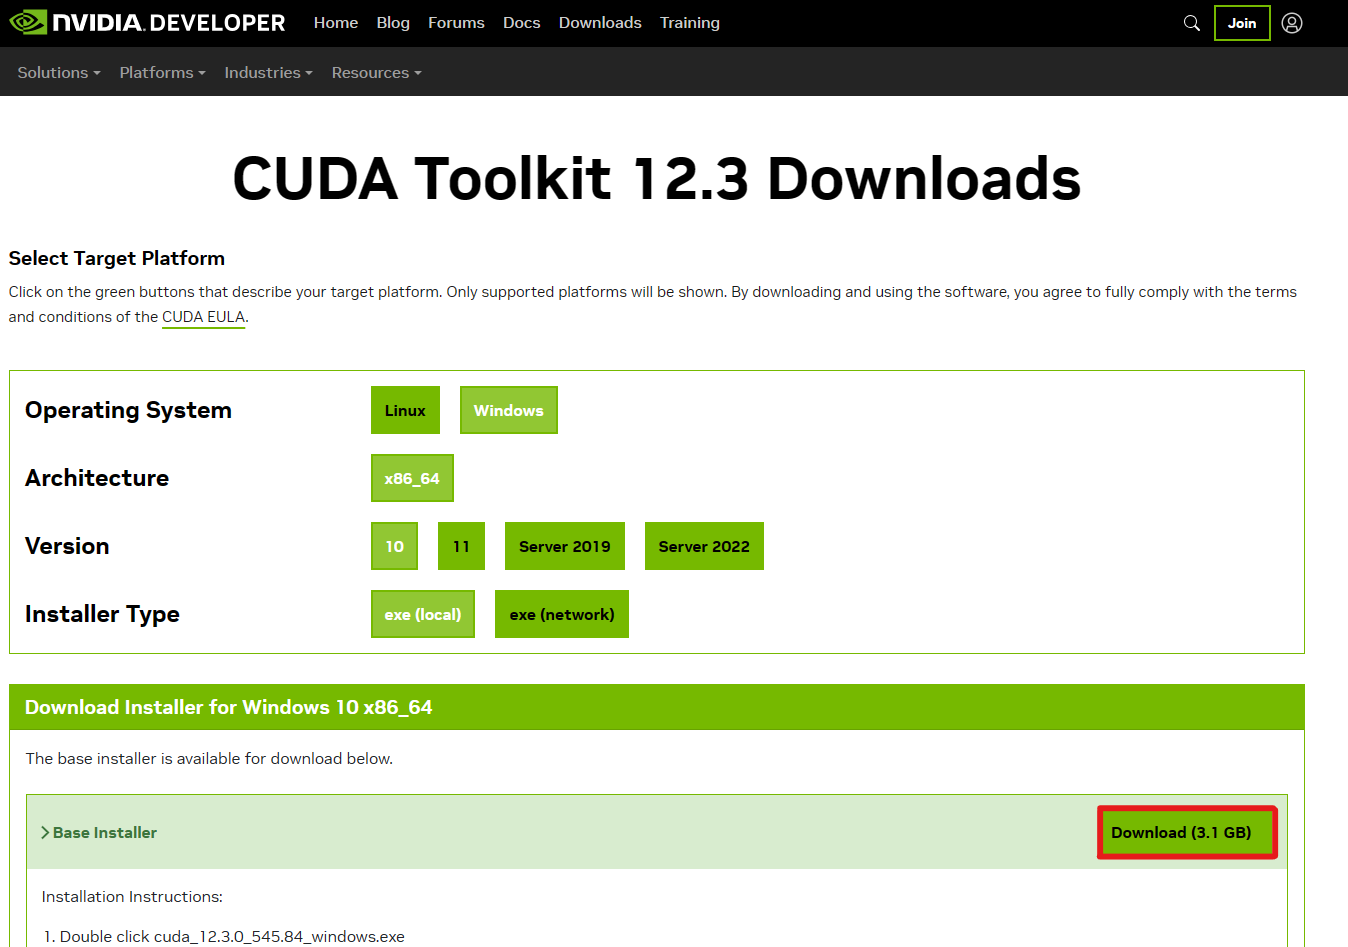
\includegraphics[width=150mm, keepaspectratio] {figures/install-1.png}
	\caption{1. lépés: A CUDA letöltése}
\end{figure}

\paragraph{Új projekt létrehozása}
Telepítés után ha új projekt létrehozását választjuk (File/New/Project), akkor "CUDA [verziószám] Runtime" néven kiválasztható a projekt típusának a CUDA. Adjunk neki egy nevet és egy elérési mappát, és létre is jön a projektünk.

\begin{figure}[ht!]
	\centering
	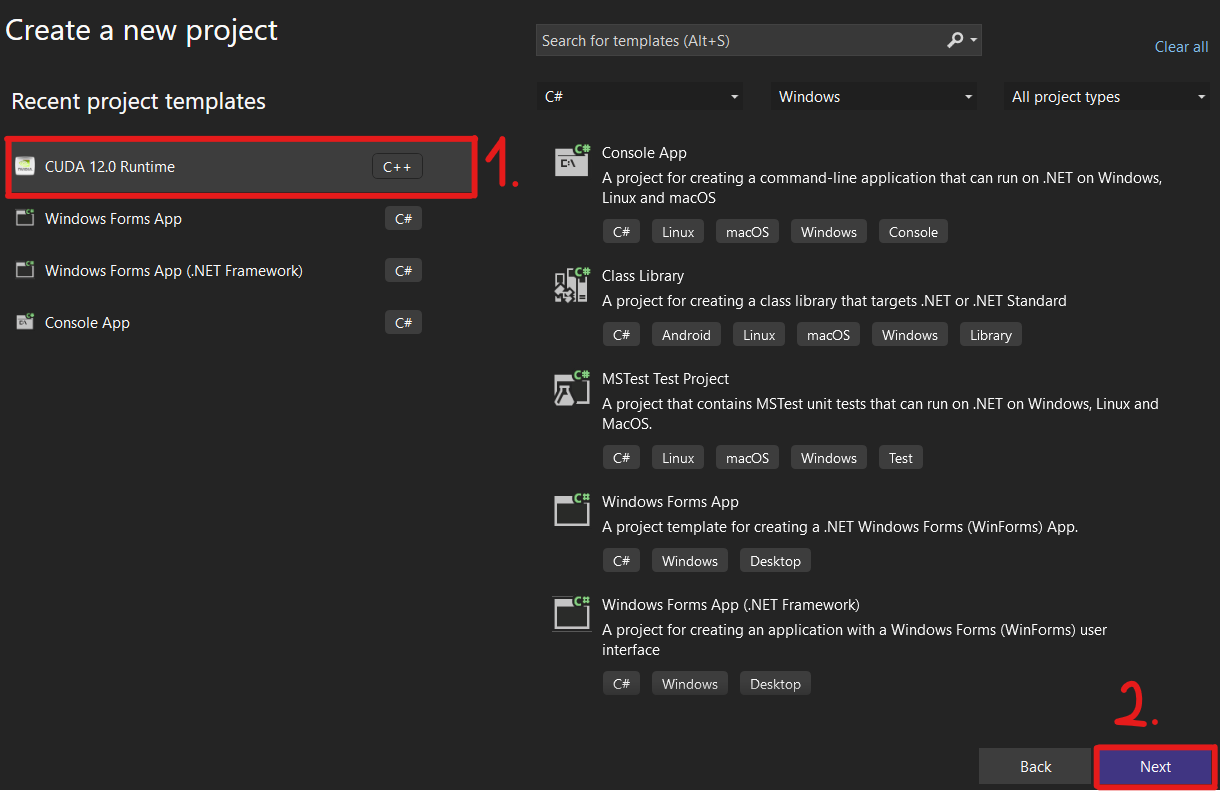
\includegraphics[width=150mm, keepaspectratio] {figures/install-2.png}
	\caption{2. lépés: Új CUDA projekt létrehozása}
\end{figure}

\paragraph{Példakód futtatása}
A template egy példaprogramot tartalmaz, amely két vektor összeadását végzi el videokártyán.

A kernel függvény nagyon egyszerű, mindössze 2 sorból áll: \cite{CUDAdoc}
\begin{lstlisting}[style=CStyle]
	__global__ void addKernel(int *c, const int *a, const int *b)
	{
		int i = threadIdx.x;
		c[i] = a[i] + b[i];
	}
\end{lstlisting} 

A "Local Windows Debugger gomb" megnyomásával lefut a kód, és meg is kapjuk az eredményt. Ezután már írhatunk saját kódot is.

\begin{figure}[ht!]
	\centering
	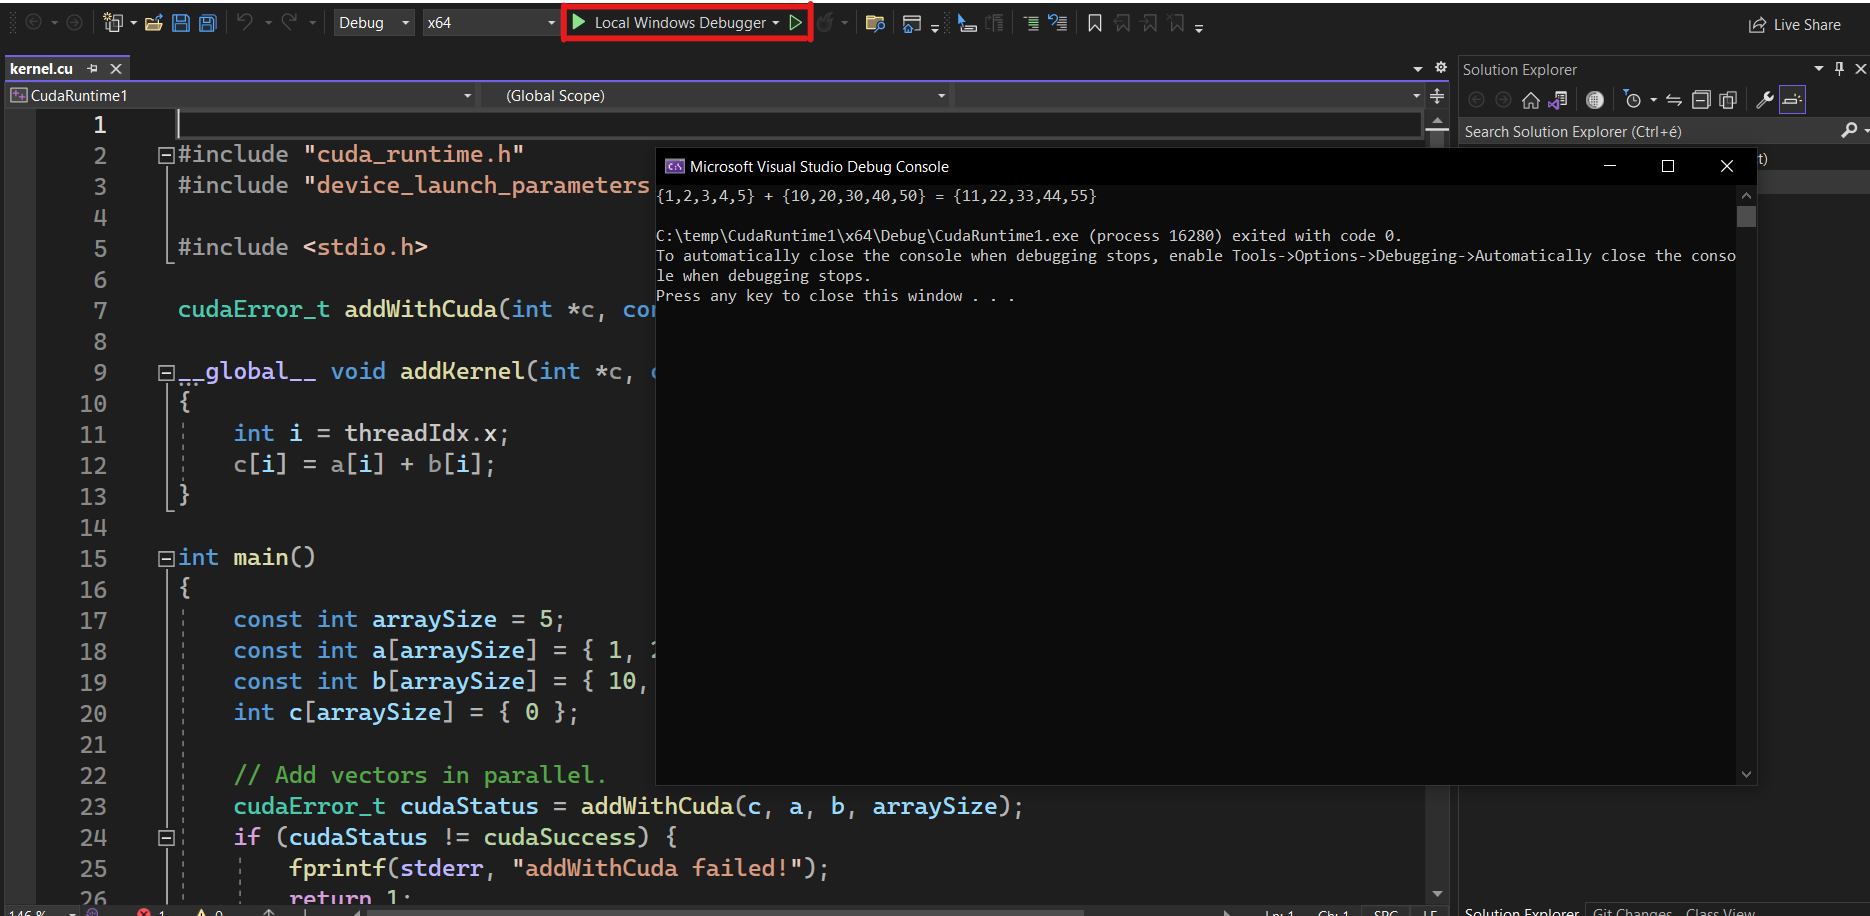
\includegraphics[width=150mm, keepaspectratio] {figures/install-3.png}
	\caption{3. lépés: Példakód futtatása}
\end{figure}
\chapter{Implementáció} \label{implementationChapter}

Vegyük górcső alá a témában végzett programozói munkámat. Összesen 4 algoritmussal foglalkoztam, amiket logikailag egymásra építve kezeltem:
TSP  \(\rightarrow\) VRP \(\rightarrow\) CVRP \(\rightarrow\) (C)VRPTW

\section{Hangyakolónia algoritmus}
A munkám során a felsorolt algoritmusok mindegyikét a hangyakolónia optimalizációval oldottam meg.

\subsection{Adatstruktúrák}
Az útvonaltervezési problémák gráfokon futnak, ezért elsődleges feladatom annak eldöntése volt, hogy milyen formában tároljam a gráfokat. Egyik legalapvetőbb megadási mód a szomszédossági mátrixával történő reprezentáció. Ennek előnye, hogy az egyes csúcsokhoz tartozó élek könnyen, direkt lekérdezhetőek, ezért a rajtuk végzett műveletek gyorsabbak lehetnek. Hátránya azonban, hogy minél kevesebb él van a gráfban, annál pazarlóbbá válik ez a megadás. Később tekintünk egyéb megadási módokat is, de most azokkal nem foglalkozok.
Az adattípusok megválasztásában eltérőek az egyes megvalósítások: az első TSP verzióban például minden lebegőpontos számot \textit{double} típusú változóban tárolok, míg a többi algoritmusnál \textit{float} adatípust alkalmazok. A váltás hátterében az áll, hogy kipróbálva az első algoritmust azt tapasztaltam, hogy nem javít érdemben a valószínűségek dupla pontosságú számítása, cserébe sokat lehet spórolni a futásidőn egyszeres pontossággal.


\subsection{Feromonok nyilvántartása}
A feromonokat az élekhez rendelem, ezért egy, az eredeti gráf topológiájával megegyező, teljes gráfban tárolom. A gráfélek eltárolása már másképpen történhet. 

\subsubsection{TSP}
A TSP során egy NxN-es mátrix által adott feromongráfon egyértelműen végrehajtható mohó algoritmus, vagyis olyan döntéshozatal-sorozat, hogy minden csúcsból abba a következő pontba megyünk, ahova a legtöbb feromon vezet (kivéve ha az a kezdőcsúcsba vezet, és még maradtak bejáratlan csúcsok). Hogy megtartsam az implementáció egyszerűségét, a TSP során tényleg NxN-es 2 dimenziós mátrixban tárolom a feromonértékeket. Tehát a TSP feromonmátrix a kezdőpillanatban a következő:

$\begin{pmatrix}
	0 & P_{0,1} & P_{0,2} & \cdots & P_{0,n-1}\\ 
	P_{1,0} & 0 & P_{1,2} & \cdots & P_{1,n-1} \\
	\vdots & & \ddots \\
	P_{n-1,0} & P_{n-1,1} & P_{n-1,2} & \cdots & 0
\end{pmatrix}$

Ahol P{\scriptsize i,j} az i-ből j-be él kezdeti feromonértéke. \( \forall i\in V(G) : P_{i,i}=0 \), mert a gráfunk egyszerű, nincs benne hurokél. Praktikusan \( P_{i,j}=0 \) ha az input gráfban \(v_{i,j}\) nincs behúzva. Ekkor már az első próbálkozások sem próbálnak meg arra menni. Ez a kikötés nem kötelező, előbb-utóbb ezen éleket úgyis elhalnának a feromonok. 

\subsubsection{VRP variánsok}
A VRP esetében kicsit bonyolultabb a helyzet. Ha felírjuk egymás után az egyes járművek bejárási sorrendjét azt láthatjuk, hogy olyan, mintha több TSP-t hajtottunk volna végre egymás után. Képzeletben majdnem ez is történt. Úgy álltam hozzá a több útvonalhoz, hogy fejben kifeszítettem őket egy nagy körré. A kezdőcsúcs helyére gondolhatjuk azt, hogy k db csúcs van ott, akik egymástól 0 távolságra vannak. A gondolatmenetemet a \ref{tsp-to-vrp}. ábrán illusztrálom. 

\begin{figure}[ht!]
	\centering
	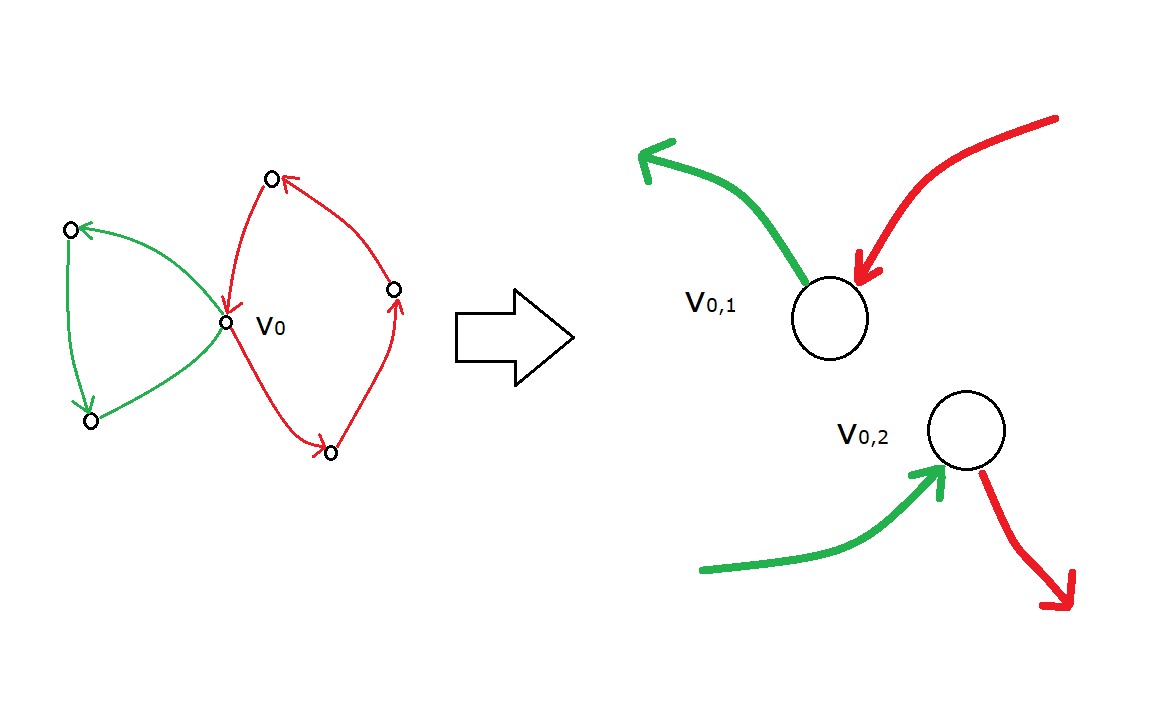
\includegraphics[width=0.5\textwidth]{figures/tsp-to-vrp.png}
	\caption{A VRP visszavezethető a TSP-re, ha az egyes utakat képzeletben összefűzzük egy nagy körré \label{tsp-to-vrp} }
\end{figure}

Egy n csúcsot k járművel bejáró VRP visszavezethető egy n+k-1 csúcsú TSP-re. Az, hogy milyen egyéb feltételeket tűzünk még ki a feladatba, a feromonok nyilvántartásának módját nem befolyásolja, csak ott módosít, hogy hiába vezet út az adott körön, ha például a járművel kapacitásfeltétele sérül. Olyankor egyáltalán nem veszem figyelembe az adott megoldást.

\textcolor{red}{BEFEJEZETLEN SZÖVEGRÉSZ}
%TODO folytani

\subsection{A rulettkerék algoritmus }
Az algoritmusaimban többször feltűnik a random számok kezelése. Hallgatótársam, Tóth Andor Márk sokat foglalkozott a témával, és diplomamunkájából sokat tanulhattam a témában \cite{alg_optim}. Valószínűségszámításból tudjuk, hogy igazi véletlen számok nem léteznek. Elméletileg nincs is semmi értelme ennek a fogalomnak. Nézzük például a klasszikus példát: a pénzérme feldobását, ami a földre érve fejjel vagy írással felfelé landol (vagy egyes nagy sikerű filmekben a sirály még a földet érés előtt elkapja és elviszi). Ha a tér minden egyes pontjában pontosan ismernénk a különböző légnyomásértékeket, valamint tökéletesen tisztában lennénk a feldobás dinamikai jellemzőivel, mindig pontosan tudnánk, hogy melyik oldalára fog esni az érme. A véletlen illúzióját ezen ismeretek hiánya okozza. Póker közben is feltehetően nem ismerjük a keverő pontos technikáját, ezért az osztott lapok jó esetben véletlenszerűnek hatnak. A számítógépek alapesetben determinisztikus gépek, hiszen adott utasításokat hajtanak végre. 
A CUDA is úgynevezett pszeudorandomszám-generátor elvét követi. Ez tökéletesen meghatározható egy kezdeti érték alapján, kell egy seed, ami viszont már független lehet a számítógéptől. Én a klasszikus megoldást választottam, miszerint az 1970. január 1. éjfél óta eltelt másodpercek számát vettem seednek.
GPU oldalon a CuRand függvénykönyvtár videokártyás támogatást biztosít pszeudorandom számok generálására, ehhez a következő egyszerű kernelt kell futtatni:

\begin{lstlisting}[style=CStyle]
	// Initializes a random seed for each different threads
	__global__ void setup_kernel(curandState* state, unsigned long seed)
	{
		int id = blockIdx.x * blockDim.x + threadIdx.x;
		curand_init(seed, id, id, &state[id]);
	}
\end{lstlisting}

A kernelt CPU oldalról kell felhívni a kiválasztott seeddel.

\begin{lstlisting}[style=CStyle]
	srand(time(0)); // Need seeds for random solutions
	
	...
	
	setup_kernel <<< BlockNum, threadPerBlock >>> (d_kernelParams.state, time(NULL) * rand());
\end{lstlisting}

\begin{lstlisting}[style=CStyle]
	
\end{lstlisting}


\section{TSP első verzió} \label{TSP_v1_SubSection}
Korábban már volt róla szó, de az útvonatkeresési algoritmusok ezen családjának legegyszerűbb tagja a TSP, ezért ezzel érdemes kezdenie annak, aki szeretne elmélyülni a problémakörben. Én is így tettem. Amikor még az Önálló laboratóriumi munkám során megismertem a genetikus algoritmusokat, az első feladatom a TSP megvalósítása volt CUDA nyelven. Azért tartom fontosnak kiemelni a TSP programom első verzióját, mert elsőkörben teljesen rendszertelenül álltam a problémához, nem tekintettem a feladatra egy nagyobb téma részeként. Ez később nehezen bővithető lett volna, ezért a következő verziókat teljesen a nulláról kellett felépítenem.

A mellékletben elérhető a teljes TSP\_v1 kód, jelenleg néhány fontosabb elemet/fogalmat szeretnék kiemelni belőle.
Bevezettem egy globális változót a hangyák (threadek) számának állítására. Jelenleg konstans, amennyiben a felhasználó egyéb számú párhuzamosítást szeretne, sajnos még bele kell nyúljon a forráskódba:

\begin{lstlisting}[style=CStyle]
	// Number of threads = number of ants
	const int ants = 1024;
\end{lstlisting}

Van még néhány olyan algoritmus paraméter, ami a futás során változatlan, viszont értékük befolyásolja a futásidőt, illetve a végeredményt. Kiszerveztem őket makróba, hogy csak egy helyen kelljen változtatni.

\begin{lstlisting}[style=CStyle]
	// Repetition constants
	#define REPETITIONS 10
	#define RANDOM_GENERATIONS 20
	#define FOLLOWER_GENERATIONS 500
	
	// Pheromon matrix constants
	#define RHO 0.75  // Reduction ratio of previous pheromon value
	#define REWARD_MULTIPLIER 100   // Reward multiplier after finding a shortest path until then
	#define INITIAL_PHEROMONE_VALUE 1000    // Initial value of elements in the Pheromone matrix
	
	#define SERIALMAXTRIES 10    // Number of serial processes
\end{lstlisting}

Először a "Repetition" konstansokról: Az algoritmus így működik: Csináld REPETITIONS alkalommal, hogy jön RANDOM\_GENERATIONS iteráció olyan hangya, aki teljesen véletlenszerűen végigmegy a gráfon, majd őket követi FOLLOWER\_GENERATIONS iterációban olyan hangya, aki a feromon alapján dönti el az útját. Minél több iterációt hajtunk végre, annál több utat vizsgálunk meg, és elvileg annál pontosabb lehet a végeredmény.
Az előbbiektől némileg elkülönül a SERIAL\_MAXTRIES, ami azért felel, hogy többször lefuttathassuk egymás után a GPU kernelt. Mivel az ACO egy heurisztikus algoritmus, futásonként más és más eredményt szolgáltat. Éppen ezért érdemes lehet többször (például 10-szer) egymás után végrehajtani az algoritmust, és megvizsgálni az egyes eredményeket. Ilyenkor végső eredménynek célszerű a legrövidebb megoldást venni. Sajnos a tesztelések során azt tapasztaltam, hogy a GPU főleg amikor több szálon dolgozik, mint ami fizikailag elérhető CUDA core formájában, gyakran hibázik, és nem vagy rosszul ír át memóriaterületeket. Azon memóriaterület, mely tárolja azt aktuális minimális szekvenciát, rendkívül ki van téve 

\textcolor{red}{Hardver ismertetése}
\textcolor{red}{Többi algoritmus ismertetése}

%TODO többi algoritmus?




\chapter{Mérési eredmények} \label{resultsChapter}

A méréseket a következő paraméterekkel rendelkező számítógépen végeztem:
\begin{itemize}
	\item	CPU: 11th Gen Intel(R) Core(TM) i5-11300H @ 3.10GHz
	\item	GPU: NVIDIA GeForce RTX 3050Ti 
	\item	RAM: 24 GB DDR4 
	\item	OS: Windows 10 Education 22H2 
	\item	Compiler: NVCC V12.0.140
	
\end{itemize}

\section{A mérések menete}
Az algoritmusokhoz külön CPU és GPU kódot készítettem. Az eljárás érdemi részét megszakítás nélkül GPU-n végeztem, míg CPU-n a kezdeti értékeket állítottam be, különböző diagnosztikai kiíratásokat végeztem, illetve a parancssori argumentumok feldolgozását kezeltem. A futásidők méréséhez az NVIDIA által készített Nsight Compute(R) programot használtam, mely több szempontból képes CUDA kerneleket elemezni: futási idő, memória kihasználtsága, grid mérete, blokk mérete, szálanként regiszterek száma és még tovább. A program futását \ref{fig:nsight-compute}. ábrán ábrázoltam. 

\begin{figure}[ht!]
	\centering
	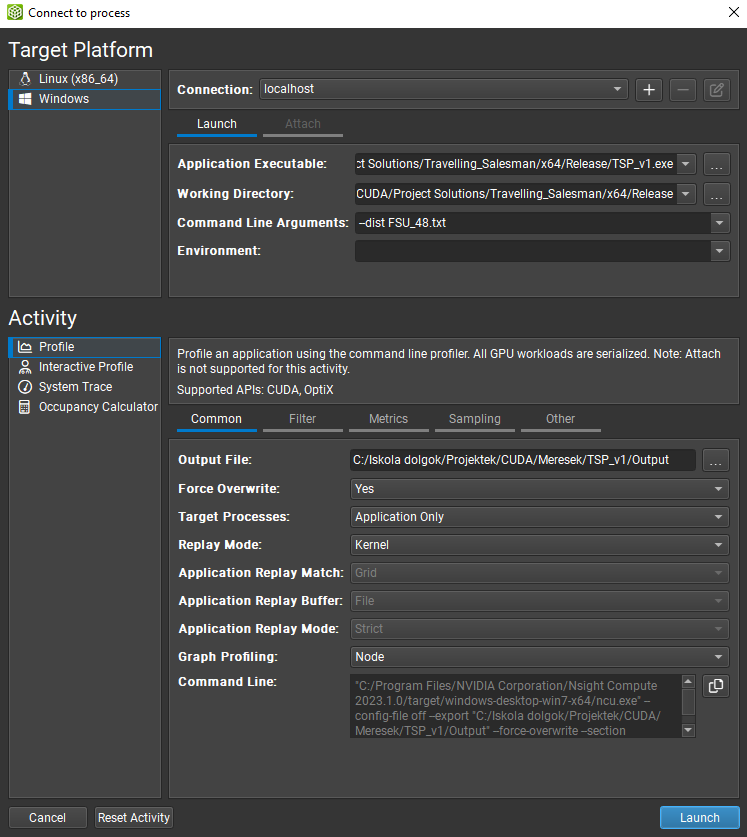
\includegraphics[width=85mm, keepaspectratio]{figures/nsight-compute-config.png}
	\caption{Az NVIDIA Nsight Compute programban egy mérés összeállításához be kell állítani a mérendő exe fájlt, a munkamappát, illetve a szükséges parancssori argumentumokat}
	\label{fig:nsight-compute-config}
\end{figure}

\begin{figure}[ht!]
	\centering
	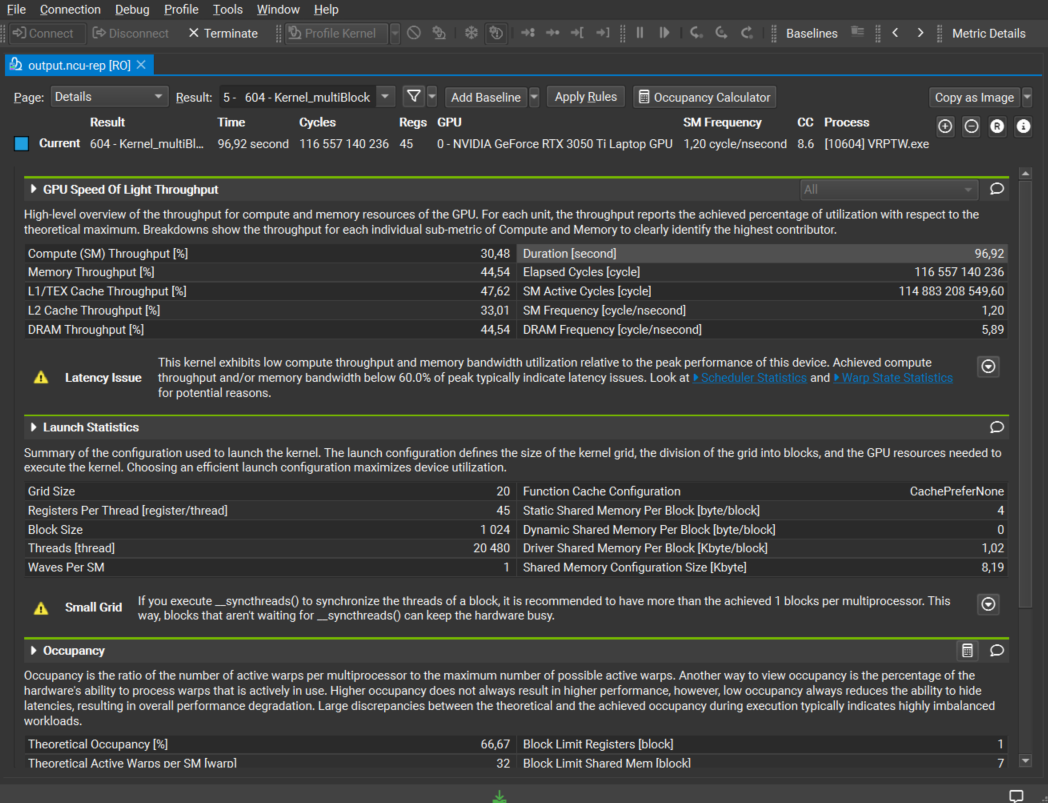
\includegraphics[width=125mm, keepaspectratio]{figures/nsight-compute2.png}
	\caption{Az NVIDIA Nsight Compute program adatok széles tárházával látja el a programozót }
	\label{fig:nsight-compute}
\end{figure}




Számomra a legfontosabb a futásidő volt, ezt több különböző bemenetre és konfigurációra lemértem, majd táblázatosan összegyűjtöttem.

\section{Mérési eredmények}

A továbbiakban táblázatokba szedtem az egyes algoritmusokon végzett profilozó méréseim eredményeit. A futásidők időegysége másodperc, mert ilyen nagyságrendben mozogtak az értékek. Többször lefuttattam a programokat ugyanolyan paraméterek mellett, ebből lejegyeztem az átlagos eredményeket (10 futás számtani közepe) és a legkisebb kapott megoldást. Amikor nem optimális egy mérési eredmény, akkor százalékos arányban melléírtam, hogy mennyivel magasabb az elméleti minimumnál.

A CVRPTW mérése során tapasztaltam először olyat, hogy néha a program egyáltalán nem talált megoldást. Ott új oszlopot vettem fel "Hiba (\%)" névvel. Azt mutatja, hogy a programfuttatások hány százalékában nem sikerült egyáltalán megoldást találni. Ilyenkor az átlagolást a sikeres futtatásokból számoltam.

\newpage
\newpage

\subsection{TSP első verzió}

Teszteléshez szükségem volt ismert eredményű adathalmazokra. A Floridai Állami Egyetem weboldalán \cite{TSPdataset} elérhető bárki számára több adathalmaz, különböző adatstruktúrában. Nekem a [fájlnév]\_d.txt nevű fájlok voltak hasznosak, ugyanis abban megtalálhatóak a szomszédossági mátrix költségei táblázatos alakban. Az itt található 6 adathalmazon végigfuttattam az algoritmusomat több konfigurációban. Mindig 10-szer ismételtem meg a futást, és lejegyeztem az eredmények átlagát (számtani középpel), illetve minimumát. Nagy adathalmaz esetén hosszú a futásidő profilozó módban, ezért időmérés céljából egyszer futtattam újra ugyanazon beállításokkal. A TSP első verziójában a feromonmátrix és az élsúlyok tárolása csak \textit{double} formátumban történik. Az összehasonlíthatóság érdekében egy iteráció során 20 random, és 500 tudatos hangya fut. A kezdeti feromon érték 1000, az elnyomási tényező \( \rho = 0.75 \), a jutalmazási arány 100, amely csak a 2. iterációtól érvényes (ha van). 

Az egyes mérések eredményei a \ref{table:TSPv1_5} - \ref{table:TSPv1_48}. táblázatokból olvashatóak.

% Size = 5
\begin{table}[ht!]
	\centering
	\begin{tabular}{|p{2cm}||p{3cm}|p{3.5cm}|p{3.5cm}|}
		\hline
		\multicolumn{4}{|c|}{FIVE : 5 csúcs, minimális út : 19, átlagos út : 24} \\
		\hline
		& Futásidő (ms) & Végeredmény átlag & Végeredmény min.\\
		\hline
		\textbf{1 rep} & & &\\
		32 ant& 7,84 & 20,2 (+6,3\%) & 19\\
		256 ant & 19,1 & 20,8 (+9,5\%) & 19\\
		1024 ant & 76,1 & 20,8 (+9,5\%) &	19\\
		\hline
		\textbf{10 rep} & & &\\
		256 ant & 137,3 & 19 &	19\\
		1024 ant & 424 &	19 &	19\\
		\hline
	\end{tabular}
	\caption{Elsőnek egy kicsi, a kezdőponton kívül 4 állomásból álló gráfon próbáltam ki az algoritmust.}
	\label{table:TSPv1_5}
\end{table}

% Size = 15
\begin{table}[ht!]
	\centering
	\begin{tabular}{|p{2cm}||p{3cm}|p{3.5cm}|p{3.5cm}|}
		\hline
		\multicolumn{4}{|c|}{P01 : 15 csúcs, minimális út : 291, átlagos út : 662} \\
		\hline
		& Futásidő (s) & Végeredmény átlag & Végeredmény min.\\
		\hline
		\textbf{1 rep} & & &\\
		1024 ant & 0,925 & 370,2 (+27,2\%) & 291 \\
		2048 ant & 1,18 & 365 (+25,4\%) & 327 (+12,4\%) \\
		4096 ant & 1,20 & 359,7 (+23,6\%) & 332 (+14,1\%)\\
		\hline
		\textbf{10 rep} & & &\\
		1024 ant & 11,39 & 350,4 (+20,4\%) & 291\\
		2048 ant & 11,47 & 328 (+12,5\%) & 295 (+1,4\%)\\
		4096 ant & 11,59 & 336,8 (+15,7\%) & 291\\
		16384 ant & 13,21 & 326,2 (+12,1\%) & 295 (+1,4\%) \\
		20480 ant & 13,46 & 323,4 (+11,1\%) & 291 \\
		\hline
	\end{tabular}
	\caption{15 csúcsú gráfon futtatott TSP v1}
	\label{table:TSPv1_15}
\end{table}

A 17 vagy nála nagyobb gráfok esetében az 1 iterációs algoritmusok már olyan rosszul teljesítettek, hogy a méréseket legalább 10 iterációval folytattam.

% Size = 17
\begin{table}[ht!]
	\centering
	\begin{tabular}{|p{2cm}||p{3cm}|p{3.5cm}|p{3.5cm}|}
		\hline
		\multicolumn{4}{|c|}{GR : 17 csúcs, minimális út : 2085} \\
		\hline
		& Futásidő (s) & Végeredmény átlag & Végeredmény min.\\
		\hline
		\textbf{10 rep} & & & \\
		1024 ant & 14,85 & 2391,3 (+14,7\%) & 2151 (+3,2\%)\\
		2048 ant & 14,88 & 2363,4 (+13,5\%) & 2085\\
		4096 ant & 14,97 & 2279,6 (+9,3\%) & 2097 (+0,6\%) \\
		8192 ant & 15,15 & 2306,4 (+10,6\%) & 2207 (+5,9\%)\\
		16384 ant & 15,49 & 2250,5 (+7,9\%) & 2085 \\
		20480 ant & 15,68 & 2221,7 (+6,6\%) & 2085 \\
		\hline
	\end{tabular}
	\caption{17 csúcsú gráfon futtatott TSP v1}
	\label{table:TSPv1_17}
\end{table}

% Size = 26
\begin{table}[ht!]
	\centering
	\begin{tabular}{|p{2cm}||p{3cm}|p{3.5cm}|p{3.5cm}|}
		\hline
		\multicolumn{4}{|c|}{FRI26 : 26 csúcs, minimális út : 937, átlagos út : 2693} \\
		\hline
		& Futásidő (s) & Végeredmény átlag & Végeredmény min.\\
		\hline
		\textbf{10 rep} & & & \\
		1024 ant & 39,72 & 1386,1 (+47,9\%) & 1249 (+33,3\%)\\
		2048 ant & 39,73 & 1367,1 (+45,9\%) & 1221 (+30,3\%) \\
		4096 ant & 39,82 & 1227,6 (+31\%) & 1121 (+19,6\%) \\
		8192 ant & 40,14 & 1158,7 (+23,7\%) & 1102 (+17,6\%) \\
		16384 ant & 40,70 & 1132,1 (+20,8\%) & 1075 (+14,7\%) \\
		20480 ant & 42,72 & 1152,3 (+23\%) & 1097 (+17,1\%) \\
		\hline
	\end{tabular}
	\caption{26 csúcsú gráfon futtatott TSP v1}
	\label{table:TSPv1_26}
\end{table}

% Size = 42
\begin{table}[ht!]
	\centering
	\begin{tabular}{|p{2cm}||p{3cm}|p{3.5cm}|p{3.5cm}|}
		\hline
		\multicolumn{4}{|c|}{DANTZIG42 : 42 csúcs, minimális út : 699, átlagos út : 3110,5} \\
		\hline
		& Futásidő (s) & Végeredmény átlag & Végeredmény min.\\
		\hline
		\textbf{10 rep} & & & \\
		1024 ant & 115,41 & 1735,7 (+148\%) & 1554 (+122\%) \\
		2048 ant & 113,94 & 1420 (+103\%) & 1252 (+79\%) \\
		16384 ant & 114,34 & 987,7 (+41\%) & 906 (+30\%) \\
		20480 ant & 113,55 & 931,6 (+33\%) & 879 (+26\%) \\
		\hline
	\end{tabular}
	\caption{42 csúcsú gráfon futtatott TSP v1}
	\label{table:TSPv1_42}
\end{table}

% Size = 48
\begin{table}[htbp!]
	\centering
	\begin{tabular}{|p{2cm}||p{3cm}|p{3.5cm}|p{3.5cm}|}
		\hline
		\multicolumn{4}{|c|}{ATT48 : 48 csúcs, minimális út : 33523, átlagos út : 157686,9} \\
		\hline
		& Futásidő (s) & Végeredmény átlag & Végeredmény min.\\
		\hline
		\textbf{10 rep} & & & \\
		1024 ant & 156,7 & 79993,2 (+139\%) & 75601 (+126\%) \\
		8192 ant & 152,82 & 56097,9 (+67\%) & 51139 (+53\%) \\
		16384 ant & 153,78 & 50197,2 (+50\%) & 47387 (+41\%) \\
		20480 ant & 154,28 & 46360,8 (+38,3\%) & 43167 (+28,77\%) \\
		\hline
	\end{tabular}
	\caption{48 csúcsú gráfon futtatott TSP v1}
	\label{table:TSPv1_48}
\end{table}

\newpage
\newpage

\subsection{TSP második (konzisztens) verzió}
Azért, hogy az előző fejezetben látott első verzióval érdemben össze tudjam hasonlítani a mostani verziót, hasonló iterációs számokat választottam: 1 rep-en belül 20 random hangyát követ 500 tudatos hangya. Az adathalmaz is az előbbi \cite{TSPdataset} helyről származó csomag. A számértékeket összevetve szembetűnő a gyorsulás az előző verzióhoz képest. A legfőbb szerepe ebben úgy gondolom, hogy az adattípus \textit{double}-ről \textit{float}-ra cserélése, illetve a függvények között szigorú pointer alapú paraméterátadás jelentette.

Az egyes mérések eredményei a \ref{table:TSPv2_15} - \ref{table:TSPv2_48}. táblázatokból olvashatóak ki.

% Size = 15
\begin{table}[ht!]
	\centering
	\begin{tabular}{|p{2cm}||p{3cm}|p{3.5cm}|p{3.5cm}|}
		\hline
		\multicolumn{4}{|c|}{P01 : 15 csúcs, minimális út : 291, átlagos út : 662} \\
		\hline
		& Futásidő (s) & Végeredmény átlag & Végeredmény min.\\
		\hline
		\textbf{10 rep} & & &\\
		1024 ant & 2,69 & 320,0 (+10\%) & 307 (+5,5\%) \\
		2048 ant & 2,82 & 307,6 (+5,7\%) & 291\\
		4096 ant & 2,97 & 305,4 (+4,9\%) & 291\\
		8192 ant & 3,19 & 300,2 (+3,2\%) & 291\\
		12288 ant & 3,50 & 296,4 (+1,9\%) & 291\\
		16384 ant & 3,73 & 294,6 (+1,2\%) & 291\\
		20480 ant & 3,92 & 295,4 (+1,5\%) & 291\\
		\hline
		\textbf{30 rep} & & &\\
		1024 ant & 8,05 & 301,6 (+3,6\%) & 291\\
		20480 ant & 13,37 & 291 & 291\\
		\hline
	\end{tabular}
	\caption{15 csúcsú gráfon futtatott TSP v2}
	\label{table:TSPv2_15}
\end{table}

% Size = 17
\begin{table}[ht!]
	\centering
	\begin{tabular}{|p{2cm}||p{3cm}|p{3.5cm}|p{3.5cm}|}
		\hline
		\multicolumn{4}{|c|}{GR : 17 csúcs, minimális út : 2085} \\
		\hline
		& Futásidő (s) & Végeredmény átlag & Végeredmény min.\\
		\hline
		\textbf{10 rep} & & & \\
		1024 ant & 3,54 & 2246 (+7,7\%) & 2094 (+0,4\%)\\
		2048 ant & 3,69 & 2237,7 (+7,3\%) & 2207 (+5,9\%)\\
		4096 ant & 3,69 & 2196,5 (+5,3\%) & 2142 (+2,7\%)\\
		8192 ant & 3,89 & 2211,5 (+6,1\%) & 2170 (+4,1\%)\\
		16384 ant & 4,37 & 2179,2 (+4,5\%) & 2129 (+2,1\%)\\
		20480 ant & 4,55 & 2175,1 (+4,3\%) & 2134 (+2,4\%) \\
		\hline
		\textbf{30 rep} & & & \\
		20480 ant & 13,38 & 2146,5 & 2103 \\
		\hline
	\end{tabular}
	\caption{17 csúcsú gráfon futtatott TSP v2}
	\label{table:TSPv2_17}
\end{table}

% Size = 26
\begin{table}[ht!]
	\centering
	\begin{tabular}{|p{2cm}||p{3cm}|p{3.5cm}|p{3.5cm}|}
		\hline
		\multicolumn{4}{|c|}{FRI26 : 26 csúcs, minimális út : 937, átlagos út : 2693} \\
		\hline
		& Futásidő (s) & Végeredmény átlag & Végeredmény min.\\
		\hline
		\textbf{10 rep} & & & \\
		1024 ant & 9,00 & 1393 (+48,7\%) & 1347 (+43,8\%)\\
		2048 ant & 9,23 & 1363,1 (+45,5\%) & 1288 (+37,5\%)\\
		4096 ant & 9,43 & 1215,3 (+29,7\%)& 1163 (+24,1\%)\\
		8192 ant & 9,72 & 1136,9 (+21,3\%) & 1055 (+12,6\%)\\
		16384 ant & 10,82 & 1104,9 (+17,8\%) & 1007 (+7,5\%) \\
		20480 ant & 11,61 & 1111,7 (+18,6\%) & 1058 (+12,9\%) \\
		\hline
		\textbf{30 rep} & & & \\
		20480 ant & 32,93 & 1098,2 (+17,2\%) & 1047 (+11,7\%) \\
		\hline
	\end{tabular}
	\caption{26 csúcsú gráfon futtatott TSP v2}
	\label{table:TSPv2_26}
\end{table}

% Size = 42
\begin{table}[ht!]
	\centering
	\begin{tabular}{|p{2cm}||p{3cm}|p{3.5cm}|p{3.5cm}|}
		\hline
		\multicolumn{4}{|c|}{DANTZIG42 : 42 csúcs, minimális út : 699, átlagos út : 3110,5} \\
		\hline
		& Futásidő (s) & Végeredmény átlag & Végeredmény min.\\
		\hline
		\textbf{10 rep} & & & \\
		1024 ant & 26,19 & 1601,3 (+129\%) & 1018 (+46\%)\\
		2048 ant & 26,61 & 1488,4 (+113\%) & 1319 (+89\%) \\
		4096 ant & 27,02 & 1286,7 (+84\%) & 1168 (+67\%)\\
		8192 ant & 27,57 & 1118,3 (+60\%) & 1004 (+44\%) \\
		16384 ant & 31,2 & 1014,7 (+45\%) & 909 (+30\%)\\
		20480 ant & 33,31 & 964,9 (+38\%) & 822 (+17,6\%) \\
		\hline
		\textbf{30 rep} & & & \\
		20480 ant & 99,83 & 972,8 (+39,2\%) & 886 (+26,75\%) \\
		\hline
	\end{tabular}
	\caption{42 csúcsú gráfon futtatott TSP v2}
	\label{table:TSPv2_42}
\end{table}

% Size = 48
\begin{table}[htbp!]
	\centering
	\begin{tabular}{|p{2cm}||p{3cm}|p{3.5cm}|p{3.5cm}|}
		\hline
		\multicolumn{4}{|c|}{ATT48 : 48 csúcs, minimális út : 33523, átlagos út : 157686,9} \\
		\hline
		& Futásidő (s) & Végeredmény átlag & Végeredmény min.\\
		\hline
		\textbf{10 rep} & & & \\
		1024 ant & 38,12 & 84660,7 (+153\%) & 67541 (+102\%) \\
		2048 ant & 38,63 & 72522,8 (+116\%) & 64969 (+94\%) \\
		4096 ant & 39,14 & 62808,6 (+87\%) & 53395 (+59\%) \\
		8192 ant & 39,69 & 59604,8 (+78\%) & 52514 (+57\%) \\
		16384 ant & 41,56 & 48618,2 (+45\%) & 46227 (+38\%)\\
		20480 ant & 41,93 & 49879,9 (+48,8\%) & 45836 (+36,7\%)\\
		\hline
		\textbf{30 rep} & & & \\
		20480 ant & 124,72 & 47562,9 (+41,9\%) & 44144 (+31,7\%) \\
		\hline
	\end{tabular}
	\caption{48 csúcsú gráfon futtatott TSP v2}
	\label{table:TSPv2_48}
\end{table}

\newpage

\subsection{VRP}
A VRP-hez először nem értettem, hogy miért nem találtam külön adathalmazt. Később megértettem, hogy mivel nincs megadva egyéb feltétel, általában teljesen mindegy, hogy hány járművet használhat az algoritmus, a legjobban akkor fog járni, ha az összes állomást ugyanazon járművel járja végig. A VRP-hez is készült külön kódimplementáció. Ez azért jó, mert amikor különböző feltételeket szabunk meg, elég azok figyelembe vételével kiegészíteni a programot.


\subsection{CVRP}
Az első feltételes útvonaltervezést igénylő algoritmus, amivel foglalkoztam a kapacitásos járműútvonal-tervezés. Adathalmazt a következő helyről szedtem: \cite{CVRPdataset}.
Az iterációk az előzőeknél látottakkal megegyezőek: 1 rep-en belül 20 random hangyát követ 500 tudatos hangya.

Az egyes mérések eredményei a \ref{table:CVRP_gr17} - \ref{table:CVRP_att48}. táblázatokból olvashatóak ki.

% Size = 17
\begin{table}[ht!]
	\centering
	\begin{tabular}{|p{2cm}||p{3cm}|p{3.5cm}|p{3.5cm}|}
		\hline
		\multicolumn{4}{|c|}{17-city problem (Groetschel): 17 csúcs, minimális út: 2685} \\
		\hline
		& Futásidő (s) & Végeredmény átlag & Végeredmény min.\\
		\hline
		\textbf{10 rep} & & & \\
		1024 ant & 2,96 & 3158,7 (+17,6\%) & 2726 (+1,5\%) \\
		16384 ant & 3,44 & 2790,4 (+3,9\%) & 2711 (+1\%) \\
		20480 ant & 3,83 & 2800,5 (+4,3\%) & 2685 \\
		\hline
		\textbf{30 rep} & & & \\
		1024 ant & 6,05 & 2975,2 (+10,8\%) & 2685\\
		16384 ant & 10,64 & 2846,2 (+6\%) & 2727 (+1,5\%) \\
		20480 ant & 13,80 & 2758,5 (+2,7\%) & 2685 \\
		\hline
		\textbf{50 rep} & & & \\
		1024 ant & 9,97 & 2927,5 (+9\%) & 2685 \\
		16384 ant & 17,64 & 2737,25 (+1,9\%) & 2685\\
		20480 ant & 18,51 & 2724,9 (+1,5\%) & 2685\\
		\hline
	\end{tabular}
	\caption{gr17: 17 csúcsú gráfon futtatott CVRP}
	\label{table:CVRP_gr17}
\end{table}

% Size = 21
\begin{table}[ht!]
	\centering
	\begin{tabular}{|p{2cm}||p{3cm}|p{3.5cm}|p{3.5cm}|}
		\hline
		\multicolumn{4}{|c|}{21-city problem (Groetschel): 21 csúcs, minimális út: 3704} \\
		\hline
		& Futásidő (s) & Végeredmény átlag & Végeredmény min.\\
		\hline
		\textbf{10 rep} & & & \\
		1024 ant & 2,96 & 5026,3 (+35,7\%) & 4389 (+18,5\%) \\
		16384 ant & 4,75 & 4217 (+13,9\%) & 4068 (+9,8\%) \\
		20480 ant & 5,72 & 4103,3 (+10,8\%) & 3903 (+5,4\%) \\
		\hline
		\textbf{30 rep} & & & \\
		1024 ant & 8,31 & 4770,5 (+28,8\%) & 4001 (+8\%) \\
		16384 ant & 12,17 & 4105,4 (+10,8\%)& 3864 (+4,3\%) \\
		20480 ant & 16,61 & 4133 (+11,6\%)& 3881 (+4,8\%) \\
		\hline
		\textbf{50 rep} & & & \\
		1024 ant & 19,76 & 4467,5 (+20,6\%)& 3758 (+1,5\%)\\
		16384 ant & 22,73 & 4259,3 (+15\%) & 4090 (+10,4\%)\\
		20480 ant & 28,03 & 4211,6 (+13,7\%)& 4053 (+9,4\%)\\
		\hline
	\end{tabular}
	\caption{gr21: 21 csúcsú gráfon futtatott CVRP}
	\label{table:CVRP_gr21}
\end{table}

% Size = 33
\begin{table}[ht!]
	\centering
	\begin{tabular}{|p{2cm}||p{3cm}|p{3.5cm}|p{3.5cm}|}
		\hline
		\multicolumn{4}{|c|}{Augerat et al: 33 csúcs, minimális út: 742} \\
		\hline
		& Futásidő (s) & Végeredmény átlag & Végeredmény min.\\
		\hline
		\textbf{10 rep} & & &\\
		1024 ant & 5,62 & 1571,62 (+111,8\%) & 1283,05 (+72,9\%)\\
		16384 ant & 8,61 & 1496,24 (+101,6\%) & 1342,16 (+80,7\%) \\
		20480 ant & 13,01 & 1470,99 (+98,3\%) & 1310,18 (+76,6\%) \\
		\hline
		\textbf{30 rep} & & & \\
		1024 ant & 22,74 & 1529,4 (+106\%)& 1351,81 (+82\%)\\
		16384 ant & 23,68 & 1375,43 (+85,3\%) & 1209,97 (+63\%)\\
		20480 ant & 35,24 & 1415,17 (+90,7\%) & 1182,57 (+59,4\%) \\
		\hline
		\textbf{50 rep} & & & \\
		1024 ant & 24,91 & 1434,34 (+93,9\%) & 1230 (+65,8\%)\\
		16384 ant & 41,26 & 1421,19 (+91,5\%) & 1361,51 (+83,5\%) \\
		20480 ant & 61,01 & 1402,18 (+89\%) & 1092,92 (+47,3\%) \\
		\hline
	\end{tabular}
	\caption{a33: 33 csúcsú gráfon futtatott CVRP}
	\label{table:CVRP_a33}
\end{table}

% Size = 48
\begin{table}[ht!]
	\centering
	\begin{tabular}{|p{2cm}||p{3cm}|p{3.5cm}|p{3.5cm}|}
		\hline
		\multicolumn{4}{|c|}{Rinaldi,Yarrow/Araque: 48 csúcs, minimális út: 40002} \\
		\hline
		& Futásidő (s) & Végeredmény átlag & Végeredmény min.\\
		\hline
		\textbf{10 rep} & & & \\
		1024 ant & 44,28 & 89736,85 (+124\%) & 56813,06 (+42\%) \\
		16384 ant & 44,86 & 83208,23 (+108\%) & 57162,13 (+43\%) \\
		20480 ant & 48,89 & 89271,67 (+123\%) & 56966,07 (+42\%) \\
		\hline
		\textbf{30 rep} & & & \\
		1024 ant & 76,93 & 81507,64 (+104\%) & 67745 (+69,4\%) \\
		16384 ant & 133,62 & 74530,89 (+86,3\%) & 58940,59 (+47,3\%) \\
		20480 ant & 146,36 & 76197,09 (+90,5\%) & 53783,10 (+34,5\%) \\
		\hline
		\textbf{50 rep} & & & \\
		1024 ant & 223,39 & 75265,07 (+88,2\%) & 58007,69 (+45\%) \\
		16384 ant & 223,5 & 69196,02 (+73\%) & 54812,73 (+37\%) \\
		20480 ant & 215,03 & 64510,92 (+61,3\%) & 56817,40 (+42\%) \\
		\hline
	\end{tabular}
	\caption{att48: 48 csúcsú gráfon futtatott CVRP}
	\label{table:CVRP_att48}
\end{table}

% Size = 72
\begin{table}[ht!]
	\centering
	\begin{tabular}{|p{2cm}||p{3cm}|p{3.5cm}|p{3.5cm}|}
		\hline
		\multicolumn{4}{|c|}{Fisher problem 11: 72 csúcs, minimális út: 237} \\
		\hline
		& Futásidő (s) & Végeredmény átlag & Végeredmény min.\\
		\hline
		\textbf{10 rep} & & & \\
		16384 ant & 110,84 & 887,96 (+275\%) & 645,34 (+172\%)\\
		20480 ant & 112,34 & 923,91 (+290\%) & 874,96 (+269\%)\\
		\hline
		\textbf{30 rep} & & & \\
		16384 ant & 292,38 & 764,31 (+223\%) & 551,81 (+133\%) \\
		20480 ant & 346,49 & 706,20 (+198\%) & 458,31 (+93\%) \\
		\hline
		\textbf{50 rep} & & & \\
		16384 ant & 478,71 & 732,96 (+209\%) & 574,85 (+143\%)\\
		20480 ant & 572,36 & 679,4 (+186\%) & 492,35 (+108\%)\\
		\hline
	\end{tabular}
	\caption{f72: 72 csúcsú gráfon futtatott CVRP}
	\label{table:CVRP_f72}
\end{table}

\newpage
\newpage
\newpage
\newpage

\subsection{CVRPTW random kereséssel} \label{CVRPTW1section}
Most már az időablakok adta bonyolítást is bevesszük a feltételek közé. Olyan adathalmazzal dolgoztam \cite{VRPTWdataset}, ami egyszerre írja elő a járművek kapacitását, illetve a célpontok készen állási és határidejét. Egy rep-en belül 500 random hangyát követ 200 tudatos hangya.

 A program tesztelése során egy korábban nem tapasztalt jelenséget észleltem: \textbf{gyakran egyáltalán nem talált megoldást a program}.
Az adathalmaz sok gráfot tartalmaz, ebből én kettőt választottam: C101 és C201. Mindkettő 101 csúcsot tartalmaz, azaz a kezdőcsúcson kívül 100 állomás van. Az algoritmus futtatható az első 25 vagy 50 pontra is. A C101 gráf esetében a különböző feltételek csak néhány klienst engednek járművenként (megközelítőleg 5-10), míg a C201 esetén szabadabbak a kritériumok. Mindkét csúcshalmazt kipróbáltam 25, 50, és 100 csúcsra is. \textbf{A 25 csúcsnál nagyobb gráfok esetében ez a megvalósítás soha nem tudott eredményt találni.}

Új oszlopként megjelent a "Hiba (\%)", mely arra utal, hogy az algoritmus a programfuttatások hány \%-ában nem talált egyáltalán megoldást. 

% Size = 26
\begin{table}[ht!]
	\centering
	\begin{tabular}{|p{1.75cm}||p{2cm}|p{3.25cm}|p{3.25cm}|p{1.5cm}|}
		\hline
		\multicolumn{5}{|c|}{C101.25: 2 csúcs, minimális út: 191,3} \\
		\hline
		& Futásidő (s) & Végeredmény átlag & Végeredmény min. & Hiba(\%) \\
		\hline
		\textbf{30 rep} &  &  &  &  \\
		20480 ant & 39,31 & 441,68 (+131\%) & 336,19 (+76\%) & 70\% \\
		\hline
		\textbf{50 rep} &  &  &  &  \\
		20480 ant & 71,45 & 357,19 (+87\%) & 346,44 (+81\%) & 60\% \\
		\hline
		\textbf{70 rep} &  &  &  &  \\
		20480 ant & 94,93 & 410,70 (+115\%) & 391,42 (+105\%) & 60\% \\
		\hline
	\end{tabular}
	\caption{A szigorúbb időablakokkal bíró adathalmaz első 26 csúcsára vett random kereséses CVRPTW mérés (a nevében a 25 arra utal, hogy 25 kliens van, és egy raktár)}
	\label{table:VRTPW_25_1}
\end{table}

% Size = 26
\begin{table}[ht!]
	\centering
	\begin{tabular}{|p{1.75cm}||p{2cm}|p{3.25cm}|p{3.25cm}|p{1.5cm}|}
		\hline
		\multicolumn{5}{|c|}{C201.25: 25 csúcs, minimális út: 214.7} \\
		\hline
		& Futásidő (s) & Végeredmény átlag & Végeredmény min. & Hiba(\%) \\
		\hline
		\textbf{30 rep} &  &  &  &  \\
		20480 ant & 41,61 & 590,41 (+175\%) & 432 (+101\%) & 70\%  \\
		\hline
		\textbf{50 rep} &  &  &  &  \\
		1024 ant & 61,89 & 477,76 (+123\%) & 452,63 (+111\%) & 70\% \\
		20480 ant & 66,97 & 398,36 (+86\%) & 322 (+50\%) & 10\% \\
		\hline
		\textbf{70 rep} &  &  &  &  \\
		20480 ant & 96,92 & 469,16 (+119\%) & 396,80 (+85\%) & 60\% \\
		\hline
	\end{tabular}
	\caption{A tágabb időablakokkal bíró adathalmaz első 26 csúcsára vett random kereséses CVRPTW mérés}
	\label{table:VRTPW_25_2}
\end{table}

% Size = x
\begin{table}[ht!]
	\centering
	\begin{tabular}{|p{1.75cm}||p{2cm}|p{3.25cm}|p{3.25cm}|p{1.5cm}|}
		\hline
		\multicolumn{5}{|c|}{Gráf neve: x csúcs, minimális út: x} \\
		\hline
		& Futásidő (s) & Végeredmény átlag & Végeredmény min. & Hiba(\%) \\
		\hline
		\textbf{10 rep} &  &  &  & \\
		20480 ant &  &  &  &  \% \\
		\hline
		\textbf{30 rep} &  &  &  & \\
		20480 ant &  &  &  &  \% \\
		\hline
		\textbf{50 rep} &  &  &  &  \\
		20480 ant &  &  &  &  \% \\
		\hline
	\end{tabular}
	\caption{}
	\label{table:VRTPW_empty}
\end{table}

\subsection{CVRPTW rendezett kereséssel}

Ahogyan azt az előző fejezetben láttuk, ha teljesen random módon keresnek útvonalat az első hangyák, közepes csúcsszám mellett is képtelenség megoldást találni. Az itteni mérési eredmények már a javított random hangyákkal ellátott CVRPTW programot mérik. A tesztadathalmaz az előzővel megegyező, C101 és C201 mellett kiegészült a C202-es gráffal is. A C202-es gráf a C201-essel azonos elhelyezkedésű csúcsokat tartalmaz, viszont eltérőek az időablakok, így jobban tudjuk nézni a kritériumfeltétel közvetlen hatását. 1 repen belül 200 random hangyát követ 500 tudatos hangya (tehát mostmár egy rep több vizsgálatot tartalmaz). Sajnálatos módon a C101-et 50 és 100 csúcsra nem tudta megoldani a program, továbbra is túl nehéz feltételnek bizonyult az időablakok ilyen szűkre vétele.

% Size = 26
\begin{table}[ht!]
	\centering
	\begin{tabular}{|p{1.75cm}||p{2cm}|p{3.25cm}|p{3.25cm}|p{1.5cm}|}
		\hline
		\multicolumn{5}{|c|}{C101.25: 26 csúcs, minimális út: 191,3} \\
		\hline
		& Futásidő (s) & Végeredmény átlag & Végeredmény min. & Hiba(\%) \\
		\hline
		\textbf{10 rep} &  &  &  & \\
		1024 ant & 19,72 & 300 (+56,8\%) & 272 (+42,3\%) &  10\% \\
		16384 ant & 24,75 & 259,4 (+35,6\%) & 242 (+26,6\%) &  10\% \\
		20480 ant & 27,3 & 252 (+31\%) & 227 (+18,7\%) &  20\% \\
		\hline
		\textbf{30 rep} &  &  &  & \\
		1024 ant & 62,43 & 278 (+45,4\%) & 264 (+38,3\%) &  10\% \\
		16384 ant & 76,5 & 242 (+26,3\%) & 216 (+12,8\%) &  20\% \\
		20480 ant & 87,72 & 240 (+25,4\%) & 233 (+22\%) &  60\% \\
		\hline
		\textbf{50 rep} &  &  &  &  \\
		1024 ant & 104,63 & 270 (+41,2\%) & 255 (+33,2\%) &  10\% \\
		16384 ant & 135,2 & 239 (+24,7\%) & 222 (+16\%) &  20\% \\
		20480 ant & 154,9 & 236,6 (+23,7\%) & 228,7 (+19,5\%) &  20\% \\
		\hline
	\end{tabular}
	\caption{A szigorúbb időablakokkal bíró C101-es gráf első 26 csúcsára vett rendezett kereséses CVRPTW mérés: sajnos nagyobb csúcsméretre továbbra sem talált megoldást}
	\label{table:VRTPW2_25_1}
\end{table}

% Size = 26
\begin{table}[ht!]
	\centering
	\begin{tabular}{|p{1.75cm}||p{2cm}|p{3.25cm}|p{3.25cm}|p{1.5cm}|}
		\hline
		\multicolumn{5}{|c|}{C201.25: 26 csúcs, minimális út: 214.7} \\
		\hline
		& Futásidő (s) & Végeredmény átlag & Végeredmény min. & Hiba(\%) \\
		\hline
		\textbf{10 rep} &  &  &  & \\
		20480 ant & 27,46 & 252,8 (+17,7\%) & 215,54 &  0\% \\
		\hline
		\textbf{30 rep} &  &  &  & \\
		20480 ant & 99,04 & 223 (+3,84\%) & 215,54 &  10\% \\
		\hline
		\textbf{50 rep} &  &  &  &  \\
		20480 ant & 164,22 & 215,54 & 215,54 &  10\% \\
		\hline
	\end{tabular}
	\caption{A tágabb időablakokkal bíró adathalmaz első 26 csúcsára vett rendezett kereséses CVRPTW mérés}
	\label{table:VRTPW2_25_2}
\end{table}

% Size = 50
\begin{table}[ht!]
	\centering
	\begin{tabular}{|p{1.75cm}||p{2cm}|p{3.25cm}|p{3.25cm}|p{1.5cm}|}
		\hline
		\multicolumn{5}{|c|}{C201.50: 51 csúcs, minimális út: 360.2} \\
		\hline
		& Futásidő (s) & Végeredmény átlag & Végeredmény min. & Hiba(\%) \\
		\hline
		\textbf{10 rep} &  &  &  & \\
		20480 ant &  &  &  &  \% \\
		\hline
		\textbf{30 rep} &  &  &  & \\
		20480 ant &  &  &  &  \% \\
		\hline
		\textbf{50 rep} &  &  &  &  \\
		20480 ant &  &  &  &  \% \\
		\hline
	\end{tabular}
	\caption{A tágabb időablakokkal bíró adathalmaz első 26 csúcsára vett rendezett kereséses CVRPTW mérés}
	\label{table:VRTPW2_50_2}
\end{table}

% Size = 100
\begin{table}[ht!]
	\centering
	\begin{tabular}{|p{1.75cm}||p{2cm}|p{3.25cm}|p{3.25cm}|p{1.5cm}|}
		\hline
		\multicolumn{5}{|c|}{C201.100: 101 csúcs, minimális út: 589.1} \\
		\hline
		& Futásidő (s) & Végeredmény átlag & Végeredmény min. & Hiba(\%) \\
		\hline
		\textbf{10 rep} &  &  &  &  \\
		20480 ant & 485 & 3154,6 (+435\%) & 2935,7 (+398\%) & 0\% \\
		\hline
		\textbf{30 rep} &  &  &  &  \\
		20480 ant & 1252 & 2629 (+346,3\%) & 1413,5 (+140\%) & 0\% \\
		\hline
		\textbf{50 rep} &  &  &  &  \\
		20480 ant & 1889 & 2003,4 (+240\%) & 1476,6 (+150\%) & 10\% \\
		\hline
		\textbf{70 rep} &  &  &  &  \\
		20480 ant & 2044 & 1570 (+167\%) & 1196,1 (+103\%) &  10\% \\
		\hline
	\end{tabular}
	\caption{}
	\label{table:VRTPW2_100_2}
\end{table}


\chapter{Eredmények értékelése, továbbfejlesztési lehetőségek} \label{results_section}
Sok mérést végeztem, amiből szeretnék levonni több konklúziót. Úgy gondolom, hogy tanulságos összevetni a két elkészített TSP verziót, illetve a járműútvonal-tervezési algoritmusok esetében megvizsgálni, hogy új feltételek felvétele milyen hatással lesz a program futása után a végeredményre.

\section{A két Utazóügynök probléma (TSP) verzió összehasonlítása}

Az első megvalósított algoritmusommal a TSP, vagyis az Utazóügynök problémát oldottam meg, segítségül hívva a már korábban látott Hangyakolónia optimalizációt. Az első verzió kellő tapasztalat hiányában készült, ezért több szempontból is problémásnak bizonyult. Ilyenek a hosszú futásidő és a korlátozott bővíthetőség. Látva a profilozó mérések eredményeit, olyan változtatásokat tudtam eszközölni, mint az adattípus cseréje \textit{float}-ra, valamint a kernelen belüli szigorú pointer szerinti paraméterátadás. A módosításoknak meglett az eredménye: hasonló végeredmények mellett \textbf{a futásidők 3-4-szer rövidebbek tudtak lenni}. Az összehasonlítás a \ref{fig:TSP-benchmark}. ábrán látható.

\begin{figure}[ht!]
	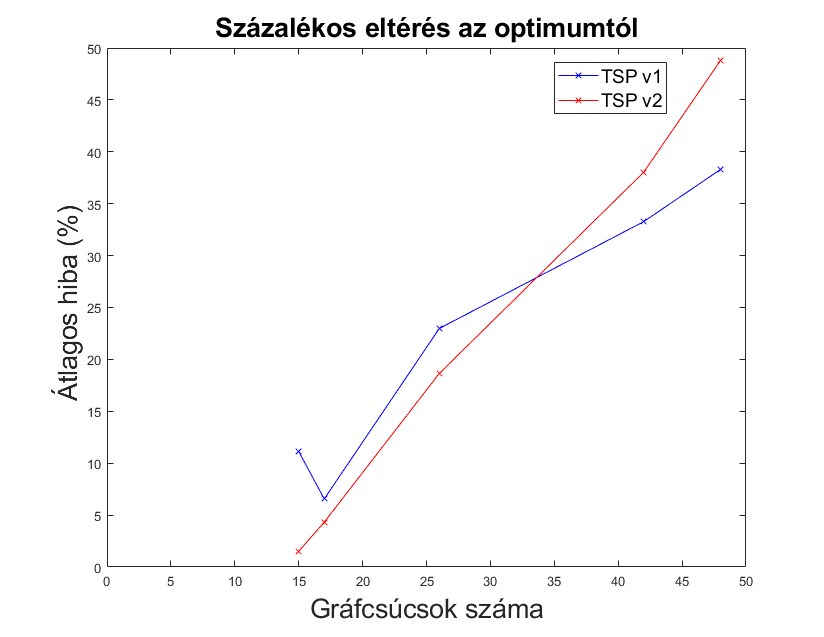
\includegraphics[width=75mm, keepaspectratio]{figures/TSP-benchmark-error.png}
	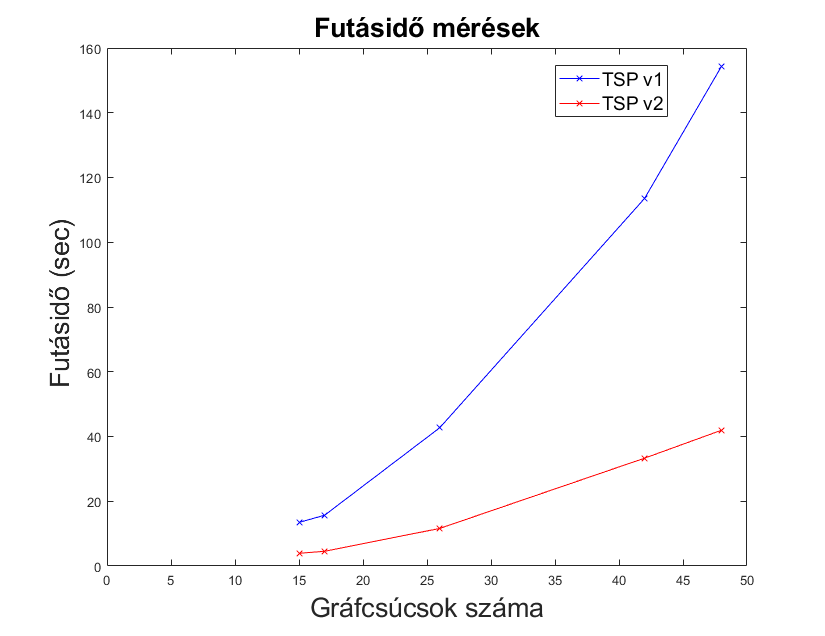
\includegraphics[width=75mm, keepaspectratio]{figures/TSP-benchmark-time.png}
	\caption{A két TSP verziót ugyanazon tesztadatokon futtattam. 20480 thread és 10 iteráció mellett Matlabban ábrázoltam a kapott eredményeket. Látható, hogy a TSP v2 hasonló eredmények mellett 3-4x gyorsabb futásra volt képes}
	\label{fig:TSP-benchmark}
\end{figure}

Mindkét implementációról elmondható, hogy jócskán felülmúlta a "Brute force" megoldást. Míg nyers összehasonlításokkal egy 48 csúcsú gráf összes lehetséges csúcssorrendjének kiértékelése évmilliókba telt volna, az ACO képes volt erre 2 perc alatt úgy, hogy az optimális megoldástól átlagosan mindössze 41,2\%-kal hosszabb utat talált, legjobb esetben csak 31,6\%-kal.
  

\section{A különböző Járműútvonal-tervezési problémák}
szép grafikonok plusz rizsa: több szál = lassabb, de jobb eredmény
%TODO értékelés

A futásidőkben gyakran nem fokozatos az emelkedés például a threadszám növelésével. Ez azért is lehet, mert időben nem egyszerre futtattam a teszteket, más volt a gép állapota, nem ugyanolyan programok futottak a háttérben stb.

\section{Kritériumfeltételek problémája a Hangyakolónia algoritmussal}
\label{section:conditionsWithACO}
Ahogy már korábban a \ref{sssec:HeldKarpEvaluate}. részben utaltam rá, a Hangyakolónia algoritmus számára is kihívással jár az, amikor a keresett útvonal különböző feltételeknek maradéktalanul meg kell feleljen. Dolgozatomban kétféle feltételrendszert vizsgáltam: a járművek korlátozott kapacitását, illetve a felhasználók megszabott időbeosztását. A CVRP esetében Most összefoglalnám, hogy miért érhettek el a feltételes esetben végzett méréseim jelentősen rosszabb eredményeket.

Az ACO úgy működik, hogy eleinte a gyengébb megoldásokból generál egyre jobbakat. Feltételezi, hogy találunk megoldást, amit javítani tudunk. A kritériumfeltételek olyanok, hogy vagy teljesülnek, vagy nem. Nehéz úgy értékelni, hogy az első csak kicsit hibázott, a következő közepesen stb. Ha rossz, akkor nem engedhetjük a megoldáshalmazba.

Most azt nézném meg, hogy ha véletlenszerű csúcssorrendeket generálok úgy, ahogyan ezt a hangyák is teszik az ACO-ban, akkor mekkora annak a valószínűsége, hogy találunk egy, a kritériumnak megfelelő megoldást.

Ha egy esemény bekövetkezési valószínűsége p, akkor annak a valószínűsége, hogy n-szer ismételve az eseményt legalább 1 alkalommal bekövetkezik, binomiális valószínűségi eloszlás szerint:
\begin{equation}
	P(x>0) = 1-(1-p)^n
	\label{binomial_probability}
\end{equation}

\subsection{Kapacitásfeltétel}
Kezdjük a kapacitáskritériummal, mert az az egyszerűbb. Az első 5 adathalmazban minden csúcs igénye 1, vagyis azt kell néztünk, hogy az egyes járművek hány csúcsot járnak be. A kezdőcsúcsot nem kell beleszámolni, mert annak nincs igénye. 

Probléma: Az (n-1) db csúcsot véletlenszerűen szétosztjuk k db jármű között. Mennyi annak a valószínűsége, hogy egyik járműhöz sem osztanak több, mint C db-ot? Első példa (gr17): 16 állomás, 3 jármű, a járművek kapacitása 6. \(p_{gr17}=?\)

\newcommand{\pgr}{0,258}

Csak 6-6-4 vagy 6-5-5 felosztásban lehetnek a csúcsok. Az összes eset \(3^{16}\), mert minden csúcsra eldöntjük, hogy melyik járműhöz osztjuk be. Összesen \(\binom{16}{6}*\binom{10}{6}*3 + \binom{16}{6}*\binom{10}{5}*3 \) esetben nem lesz több, mint 6 egyik jármű kapacitása sem.
\begin{equation}
	p_{gr17} = 3*\frac{\binom{16}{6}*\binom{10}{6} + \binom{16}{6}*\binom{10}{5}}{3^{16}} \approx \pgr
	\label{gr17_p}
\end{equation}
Nézzük meg az att48-ra is ugyanezt: \((n-1)=47\) állomás, k=3 jármű, a járművek kapacitása C=16. \(p_{att48}=?\)

\newcommand{\patt}{0,051}

Ebben a problémában csak 16-16-15 felosztásban lehetnek a csúcsok. Az előbbi példához hasonlóan gondolkozva a valószínűség:

\begin{equation}
	p_{gr17} = \frac{3*\binom{47}{16}*\binom{31}{16}}{3^{47}} \approx \patt
	\label{att48_p}
\end{equation}

\newcommand{\nInTenIterations}{4096000}

Ha 20480 szálon 10 iterációt végzek, és 1 iteráción belül 20-szor generálok egymás után random sorrendet, akkor összesen n=\nInTenIterations kísérletet végzek. A \ref{binomial_probability}. egyenletbe behelyettesítve annak a valószínűsége, hogy találok megoldást:

\begin{equation}
	P_{gr17} = 1-(1-\pgr)^{\nInTenIterations} = 1
	\label{gr17_P}
\end{equation}

\begin{equation}
	P_{att48} = 1-(1-\patt)^{\nInTenIterations} = 1
	\label{att48_P}
\end{equation}

Ezek alapján nem meglepő, hogy mindig találtam megoldást a CVRP tesztelése során.

\subsection{Időablakok feltétele}
Most jön annak a vizsgálata, hogy miért nem találtam megoldást olyan sok esetben a CVRPTW mérésekor. Sajnos itt már nem lehet olyan szépen intuitívan megállapítani egy adott problémában egy véletlenszerű bejárás megfelelőségének a valószínűségét. 
\include{content/osszefoglalas.tex}


% Acknowledgements
%~~~~~~~~~~~~~~~~~~~~~~~~~~~~~~~~~~~~~~~~~~~~~~~~~~~~~~~~~~~~~~~~~~~~~~~~~~~~~~~~~~~~~~
%----------------------------------------------------------------------------
\chapter*{\koszonetnyilvanitas}\addcontentsline{toc}{chapter}{\koszonetnyilvanitas}
%----------------------------------------------------------------------------

Szeretném kifejezni hálás köszönetemet konzulensemnek, Dr. Szegletes Lucának, aki már a Témalaboratórium tárgy óta segítséget nyújtott a munkámhoz. Nagyon sokat jelentett nekem, hogy családom és barátaim észrevételeikkel támogattak abban, hogy dolgozatom helyesírási hibáktól mentesebb lehessen. Továbbá hálás vagyok Andy Sambergnek a Brooklyn 99 című sorozat elkészítéséért, mely sok örömöt okozott dolgozatírás közben.


% List of Figures, Tables
%~~~~~~~~~~~~~~~~~~~~~~~~~~~~~~~~~~~~~~~~~~~~~~~~~~~~~~~~~~~~~~~~~~~~~~~~~~~~~~~~~~~~~~
%\listoffigures\addcontentsline{toc}{chapter}{\listfigurename}
%\listoftables\addcontentsline{toc}{chapter}{\listtablename}


% Bibliography
%~~~~~~~~~~~~~~~~~~~~~~~~~~~~~~~~~~~~~~~~~~~~~~~~~~~~~~~~~~~~~~~~~~~~~~~~~~~~~~~~~~~~~~
\addcontentsline{toc}{chapter}{\bibname}
\bibliography{bib/mybib}


% Appendix
%~~~~~~~~~~~~~~~~~~~~~~~~~~~~~~~~~~~~~~~~~~~~~~~~~~~~~~~~~~~~~~~~~~~~~~~~~~~~~~~~~~~~~~
%----------------------------------------------------------------------------
\appendix
%----------------------------------------------------------------------------
\chapter*{\fuggelek}\addcontentsline{toc}{chapter}{\fuggelek}
\setcounter{chapter}{\appendixnumber}
%\setcounter{equation}{0} % a fofejezet-szamlalo az angol ABC 6. betuje (F) lesz
\numberwithin{equation}{section}
\numberwithin{figure}{section}
\numberwithin{lstlisting}{section}
%\numberwithin{tabular}{section}
%----------------------------------------------------------------------------
\section{A megvalósított CUDA kódok elérése}
%----------------------------------------------------------------------------
Jelen dolgozat készítése során több CUDA keretrendszer segítségével több programot is írtam. Ezek forráskódját nyilvánosan elérhetővé tettem, a következő github linken elérhető a tesztadatokkal együtt: https://github.com/jost1234/VRPwithCUDA

\begin{figure}[!ht]
\centering
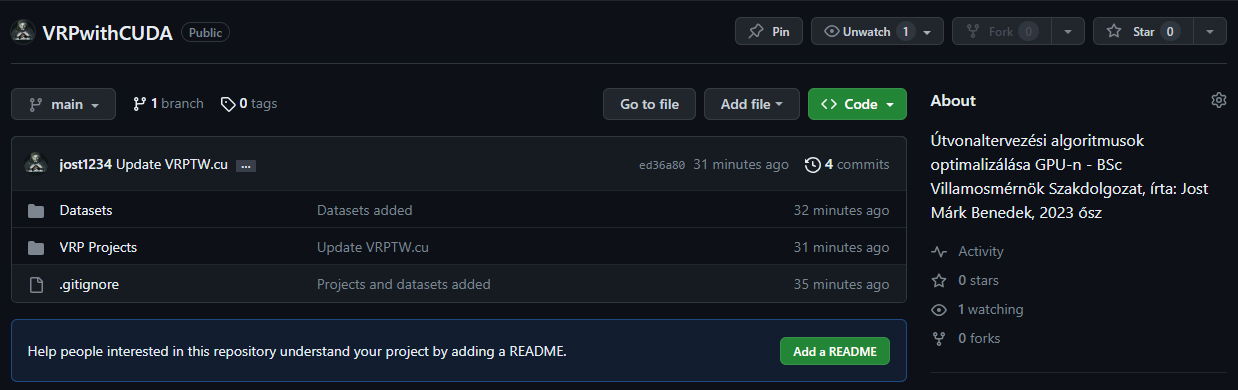
\includegraphics[width=150mm, keepaspectratio]{figures/github.png}
\caption{A dolgozat során készített CUDA projektek szabadon megtekinthetően githubon \href{https://github.com/jost1234/VRPwithCUDA}{IDE KATTINTVA}}
\label{fig:github} 
\end{figure}


%----------------------------------------------------------------------------
%\clearpage\section{A dolgozat során használt rövidítések}
%----------------------------------------------------------------------------



%\label{page:last}
\end{document}
